% Plain-language review document (explaneat plain-language review), v5.
\documentclass[a4paper,10pt]{article}
\usepackage[margin=1.8cm]{geometry}
\usepackage{amsmath}
\usepackage{amssymb}
\usepackage{booktabs}
\usepackage{tabularx}
\usepackage{graphicx}
\usepackage[table,usenames,dvipsnames]{xcolor}
\usepackage{tikz}
\usetikzlibrary{arrows.meta,fit,backgrounds,positioning,calc}
\usetikzlibrary{shapes.geometric}
\usepackage{longtable}
\usepackage{pdflscape}
\usepackage{float}
\usepackage[font=small,labelfont=bf]{caption}
\usepackage{array}
\usepackage[unicode=true,hidelinks]{hyperref}
\setcounter{tocdepth}{3}
\setcounter{secnumdepth}{3}
% Review markers, copied from dissertation.tex (7 Nov 2026) for standalone builds.
\newif\ifreviewmarks
\reviewmarkstrue
\newcommand{\reviewrule}{\noindent{\color{BrickRed}\rule{\linewidth}{0.8pt}}}
\newenvironment{drafted}[1][]{%
  \ifreviewmarks\par\addvspace{\medskipamount}\reviewrule\par\nopagebreak
  \noindent{\color{BrickRed}\sffamily\footnotesize\textbf{Thesis Draft}\quad #1\hfill review}\par\nopagebreak\smallskip\fi}{%
  \ifreviewmarks\par\smallskip\noindent{\color{BrickRed}\sffamily\footnotesize end of thesis draft}\par\nopagebreak\reviewrule\par\medskip\fi}
\newcommand{\figreview}[1]{\ifreviewmarks\par\smallskip{\color{NavyBlue}\sffamily\footnotesize\textbf{Figure note:} #1}\par\fi}
\begin{document}
\begin{center}{\Large\bfseries Plain-language explanation: churn100-s2-c2\par}\vspace{2mm}{\small AI-assisted drafts for review. Nothing here has been verified by a person.\par}\end{center}
\noindent\textbf{How to read this.} Explanations are built up but read down: the summary first, then each part from the whole model down, in plain words, each sentence followed by the claims it rests on (C01, C02, \ldots; every cited claim was computed on the model and checked). Numbers are changes in predicted risk for a typical patient. The technical record (original hypotheses, formulas, evidence tables with the test check, ranges and n) is at the end. The text describes what the model does, not the world; whether it is plausible is for the reviewer to judge.
\par\medskip\noindent\textbf{What changed in v5e (figures).} v5e: every diagram is a numbered figure with a caption (list of figures after the contents) and the text refers to it; the whole-network figure has its own landscape page, scaled to the page, with a short caption and its description in the text; an input used by several parts is drawn under each of them (same input, repeated for readability, dotted outline); and an appendix figure shows the trained network before any explanation (no parts, no splits).
\par\medskip\noindent\textbf{What changed in v5c (tables and diagrams).} v5c: the evidence tables are landscape, compact and shaded by row, with the header repeated on every page (longtable and pdflscape, used in this review PDF only; the thesis preamble has neither). In the diagrams each input is drawn once, in a shared row along the bottom (the explanation's split copies of an input are listed in the technical detail instead), every cluster has one output rectangle with its plain name, the inputs that feed the output directly meet in a drawn 'sum', and a one-line legend explains the edges.
\par\medskip\noindent\textbf{What changed in v5b (diagrams).} v5b uses one grouping everywhere, the annotation hierarchy: the summary's diagram is the same picture as the whole model's section, and a part that is itself a weighted sum (blood pressure with cholesterol) is a part of its own, described as one that adds up, so the text counts three parts throughout; the lint checks every 'N parts' against the hierarchy. A full-structure diagram follows the summary: every node and connection, nested by part, with the inputs that feed the output directly in their own cluster and the unused input columns listed. Each section from the top down adds its own region of that diagram, with stubs for connections from or to other parts; each connection is drawn in exactly one section. The gate's text now says that it lowers the risk for the patients it acts on, and that more vessels and higher cholesterol take that lowering away; its vessel statements are one per group.
\par\medskip\noindent\textbf{What changed in v5 (read down).} v5 reads the explanation down. The summary (one line, a diagram, one paragraph per block) is as in v4, except that the paragraph on what adds up is split into protective items, risk-raising items and rare results, and an input that also feeds a part is quoted with its direct contribution only (the rest is in that part's paragraph). Then the document walks the annotation hierarchy from the whole model down: for each part a plain hypothesis (what it does for the prediction), plain evidence (what was checked and what it showed; for a part made of others, what they are and how they combine), a diagram one level down and where to read on. The original hypotheses, closed forms and evidence tables are in 'Technical detail' at the end. Statements about structure (what a part is made of, a copy of another part, a formula that reproduces it) are now claims of their own, checked on the graph and the data.
\par\medskip\noindent\textbf{v4.} v4 follows the structure of the explanation. The summary opens with one line and a diagram at the same grouping, then gives one paragraph per top-level block of the annotation hierarchy: one for everything that adds up independently (the inputs that feed the model score directly, and parts that are a weighted sum), and one for each part that combines its inputs in another way: what it combines, how, and for whom. 'Parts in detail' follows the hierarchy below that, with a diagram one level down for each part that contains others. The prose no longer says 'clearly', 'slightly', 'consistently' or 'on the training data only': the numbers carry it, and the test check, the ranges and n stay in the evidence tables. Only genuinely small groups are marked, with their n. The lint rejects the confidence words and checks the block structure.
\tableofcontents
\listoffigures
\clearpage
\begin{drafted}[plain-language layer: churn100-s2-c2]
\section{churn100-s2-c2}
\noindent{\small Genome \texttt{e5394267-5807-44ae-8629-5e157bcfb43a}, explanation \texttt{4792056e-ee3e-4fde-a1bb-4c4d809e2d61}. Split: train primary (n=4000), test as a check (n=1000). Claims: 147, verified 138, not supported 9.\par}
\noindent{\small\textcolor{BrickRed}{AI-assisted draft for review (unverified)}\par}\smallskip
\noindent{\footnotesize Reference (typical) customer: the typical customer: the median training customer for every number and the most common training category for every category (not a real customer). account length: 100; area code: area code 415; international plan: no international plan; number customer service calls: 1 calls; number vmail messages: 0 messages; state: West Virginia; total day calls: 100 calls; total day charge: 30.69 US dollars; total day minutes: 180 minutes; total eve calls: 100 calls; total eve charge: 17.12 US dollars; total eve minutes: 201 minutes; total intl calls: 4 calls; total intl charge: 2.78 US dollars; total intl minutes: 10 minutes; total night calls: 100 calls; total night charge: 9.02 US dollars; total night minutes: 200 minutes; voice mail plan: no voice-mail plan. Predicted chance that a customer leaves: 1\%.\par}
\subsection{Summary}
\noindent For a typical customer (in West Virginia, area code 415, no international or voice-mail plan, 1 call to customer service and median usage) the model predicts a chance of leaving of about 1\%; it adds up six parts: fixed-weight inputs, service calls, a voice-mail discount, state units, an area-code unit and a small Utah unit.\,{\scriptsize\textcolor{NavyBlue}{[C051]}} Figure~\ref{fig:churn100s2c2:summary} shows the model at this level: one box per paragraph below.
\par\medskip\noindent\fbox{\begin{minipage}{0.96\linewidth}\small\textbf{How to read the diagrams.} Edge colour is the sign of that one connection: blue positive, red negative; thicker is a larger weight. The outline and arrow on an input (and on a part's output box) is its overall effect on the final prediction, read from the verified claims: orange and up arrow raises it, teal and down arrow lowers it, grey and double arrow depends (it goes both ways, or differs between levels). A negative connection into a part that itself raises the prediction means that input lowers the prediction; through a hinge the overall effect can only be read from the claims, not from the edges. Up arrow means towards churn; down arrow, away from it. A double outline marks an input (or a part's output) that acts at a fixed rate everywhere: it adds the same amount to the score per unit, so it is explained by its rate alone (see 'Linear factors'); a dashed double outline, at a fixed rate on the observed data. The normal outline is an input whose effect switches on and off somewhere. For example, total daytime minutes has a negative connection into 'Service calls', a part that raises the predicted chance that a customer leaves, so total daytime minutes lowers it.\end{minipage}}\par\medskip
\begin{figure}[H]\centering
\resizebox{!}{\ifdim\height>0.5\textheight 0.5\textheight\else\height\fi}{%
\resizebox{\ifdim\width>\linewidth\linewidth\else\width\fi}{!}{%
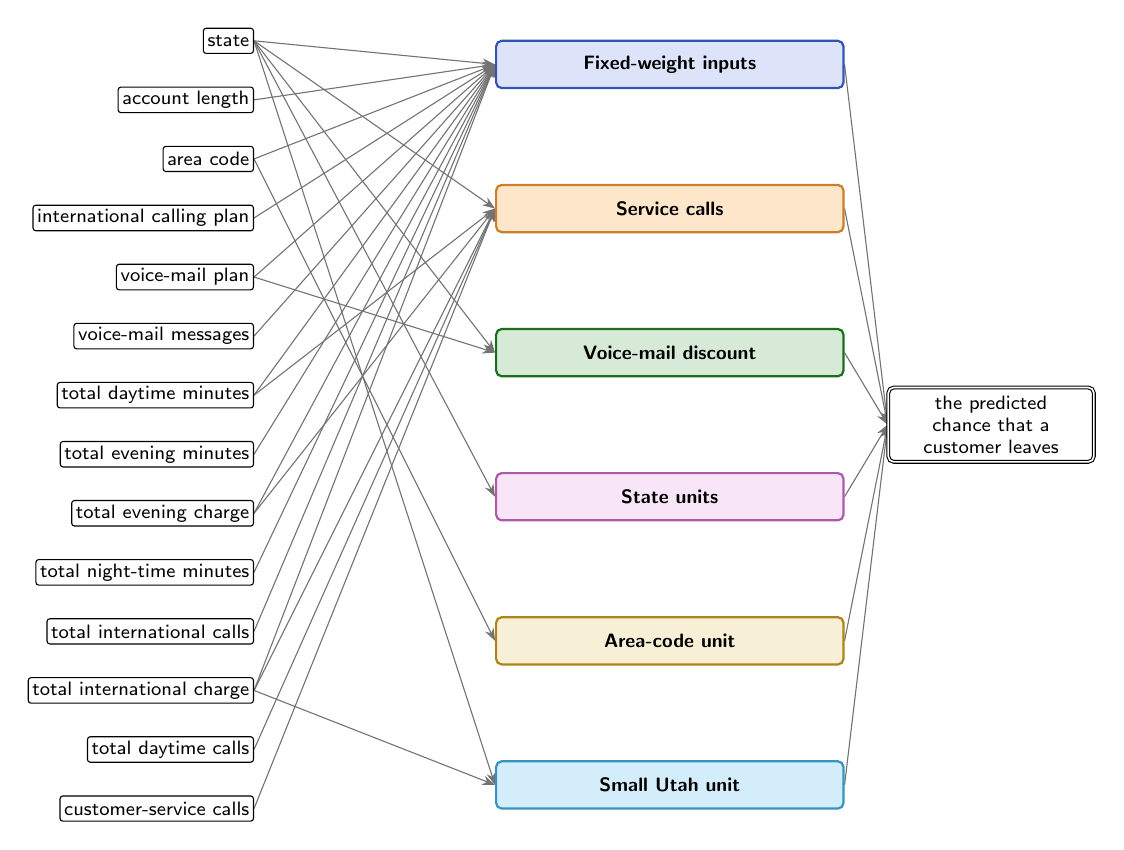
\begin{tikzpicture}[
  font=\sffamily\scriptsize, >={Stealth[length=1.6mm]},
  inp/.style={draw, rounded corners=1pt, fill=white, inner sep=1.5pt, minimum height=3.2mm, anchor=east},
  abox/.style={draw, thick, rounded corners=2pt, align=center, inner sep=3pt, minimum height=6mm, text width=42mm},
  outp/.style={draw, double, rounded corners=2pt, fill=white, align=center, inner sep=3pt, text width=24mm},
  agg/.style={draw=black!55},
]
\node[inp] (i0) at (0,4.875) {state};
\node[inp] (i1) at (0,4.125) {account length};
\node[inp] (i2) at (0,3.375) {area code};
\node[inp] (i3) at (0,2.625) {international calling plan};
\node[inp] (i4) at (0,1.875) {voice-mail plan};
\node[inp] (i5) at (0,1.125) {voice-mail messages};
\node[inp] (i6) at (0,0.375) {total daytime minutes};
\node[inp] (i7) at (0,-0.375) {total evening minutes};
\node[inp] (i8) at (0,-1.125) {total evening charge};
\node[inp] (i9) at (0,-1.875) {total night-time minutes};
\node[inp] (i10) at (0,-2.625) {total international calls};
\node[inp] (i11) at (0,-3.375) {total international charge};
\node[inp] (i12) at (0,-4.125) {total daytime calls};
\node[inp] (i13) at (0,-4.875) {customer-service calls};
\node[abox, fill=RoyalBlue!18, draw=RoyalBlue!80!black] (b0) at (5.28,4.575) {\textbf{Fixed-weight inputs}};
\node[abox, fill=BurntOrange!18, draw=BurntOrange!80!black] (b1) at (5.28,2.745) {\textbf{Service calls}};
\node[abox, fill=ForestGreen!18, draw=ForestGreen!80!black] (b2) at (5.28,0.915) {\textbf{Voice-mail discount}};
\node[abox, fill=Orchid!18, draw=Orchid!80!black] (b3) at (5.28,-0.915) {\textbf{State units}};
\node[abox, fill=Goldenrod!18, draw=Goldenrod!80!black] (b4) at (5.28,-2.745) {\textbf{Area-code unit}};
\node[abox, fill=Cerulean!18, draw=Cerulean!80!black] (b5) at (5.28,-4.575) {\textbf{Small Utah unit}};
\node[outp] (out) at (9.36,0) {the predicted chance that a customer leaves};
\begin{scope}[on background layer]
\draw[->, agg, thin] (i0.east) -- (b0.west);
\draw[->, agg, thin] (i1.east) -- (b0.west);
\draw[->, agg, thin] (i2.east) -- (b0.west);
\draw[->, agg, thin] (i3.east) -- (b0.west);
\draw[->, agg, thin] (i4.east) -- (b0.west);
\draw[->, agg, thin] (i5.east) -- (b0.west);
\draw[->, agg, thin] (i6.east) -- (b0.west);
\draw[->, agg, thin] (i7.east) -- (b0.west);
\draw[->, agg, thin] (i8.east) -- (b0.west);
\draw[->, agg, thin] (i9.east) -- (b0.west);
\draw[->, agg, thin] (i10.east) -- (b0.west);
\draw[->, agg, thin] (i11.east) -- (b0.west);
\draw[->, agg] (b0.east) -- (out.west);
\draw[->, agg, thin] (i0.east) -- (b1.west);
\draw[->, agg, thin] (i6.east) -- (b1.west);
\draw[->, agg, thin] (i12.east) -- (b1.west);
\draw[->, agg, thin] (i8.east) -- (b1.west);
\draw[->, agg, thin] (i11.east) -- (b1.west);
\draw[->, agg, thin] (i13.east) -- (b1.west);
\draw[->, agg] (b1.east) -- (out.west);
\draw[->, agg, thin] (i0.east) -- (b2.west);
\draw[->, agg, thin] (i4.east) -- (b2.west);
\draw[->, agg] (b2.east) -- (out.west);
\draw[->, agg, thin] (i0.east) -- (b3.west);
\draw[->, agg] (b3.east) -- (out.west);
\draw[->, agg, thin] (i2.east) -- (b4.west);
\draw[->, agg] (b4.east) -- (out.west);
\draw[->, agg, thin] (i0.east) -- (b5.west);
\draw[->, agg, thin] (i11.east) -- (b5.west);
\draw[->, agg] (b5.east) -- (out.west);
\end{scope}
\end{tikzpicture}}}%
\caption{The model at the level of the summary: one box per part.}
\label{fig:churn100s2c2:summary}
\end{figure}
\paragraph{Fixed-weight inputs.} This part adds up most inputs with fixed weights, and daytime minutes count most: they raise a typical customer's chance of leaving steadily, from under 1\% at 112 to about 11\% at 249 minutes.\,{\scriptsize\textcolor{NavyBlue}{[C053]}} An international plan takes the chance from about 1\% to about 14\%, a voice-mail plan lowers it to under 1\%, and more voice-mail messages raise it steadily, from about 1\% at 0 to about 4\% at 32 messages.\,{\scriptsize\textcolor{NavyBlue}{[C052, C061, C056]}} A higher international charge, more evening minutes, a higher evening charge and more night-time minutes also raise it steadily, each by one to two points.\,{\scriptsize\textcolor{NavyBlue}{[C057, C059, C060, C065]}} Through it, the state moves the chance from about 1\% in West Virginia to about 5\% in Washington and in California, and to under 1\% in Hawaii (41 to 122 training customers per state).\,{\scriptsize\textcolor{NavyBlue}{[C054, C055, C062]}}
\paragraph{Service calls.} This part adds up two parts: customer-service calls combined with low daytime use, and a rise from 4 calls upwards.\,{\scriptsize\textcolor{NavyBlue}{[C103]}} Through it, daytime minutes lower the chance only while they stay below about 166 minutes (between 145 and 213 minutes for different customers), in an uneven way: for a typical such customer, from about 28\% at 91 minutes to about 1\% at 352 minutes.\,{\scriptsize\textcolor{NavyBlue}{[C098]}} With an evening charge above 17.12 US dollars, the chance is lowest at about 148 minutes of daytime use and higher either side: from about 1\% at 112 minutes to about 13\% at 249 minutes, against about 2\% to about 9\% at or below that charge.\,{\scriptsize\textcolor{NavyBlue}{[C095]}} Customer-service calls add to it from 4 calls upwards, slowly at first, then faster: for a typical such customer, from about 3\% at 0 calls to about 8\% at 4 calls.\,{\scriptsize\textcolor{NavyBlue}{[C099]}}
\paragraph{Voice-mail discount.} This part reads the voice-mail plan and one state: through it, a voice-mail plan lowers a typical customer's chance from about 1\% to under 1\%, and customers in North Carolina get under 1\% instead of about 1\%.\,{\scriptsize\textcolor{NavyBlue}{[C119, C120]}}
\paragraph{State units.} This part reads only the state: it raises a typical customer's chance from about 1\% to about 2\% in Washington and in Montana, and by less than a point in Kentucky and Ohio.\,{\scriptsize\textcolor{NavyBlue}{[C125, C126, C127, C128]}}
\paragraph{Area-code unit.} This part reads the area code and barely changes the predictions (by at most half a point).\,{\scriptsize\textcolor{NavyBlue}{[C137]}}
\paragraph{Small Utah unit.} This small part reads the international charge and being in Utah, and barely changes the predictions (by at most 0.2 points).\,{\scriptsize\textcolor{NavyBlue}{[C144]}}
\paragraph{The whole network.} Figure~\ref{fig:churn100s2c2:overview} (next page, landscape) draws every unit and connection of the explained model, nested by part: shaded clusters are the parts of the model and darker boxes the parts inside them; circles are hidden units (h1, h2, \ldots); each cluster's rectangle is its output, and a dashed `sum' stands for an addition the next unit does (drawn, not a unit of the model); the hexagon is the model's output. An input used by several parts is drawn under each of them (same label, dotted outline, the first copy marked with the number of copies): it is the same input, repeated for readability. Not used by the model (input columns with no connection): state: 25 of 51 levels, total daytime charge, total evening calls, total night-time calls, total night-time charge, total international minutes.
\begin{landscape}
\begin{figure}[p]\centering
\resizebox{\linewidth}{!}{%
\definecolor{netup}{HTML}{D95F02}\definecolor{netdown}{HTML}{1B9E77}\definecolor{netmixed}{HTML}{7F7F7F}%
\begin{tikzpicture}[
  font=\sffamily\scriptsize, >={Stealth[length=1.4mm]},
  inp/.style={draw, circle, fill=white, minimum size=3.2mm, inner sep=0pt},
  hid/.style={draw, circle, fill=white, minimum size=5.2mm, inner sep=0.5pt, font=\sffamily\tiny},
  exitbox/.style={draw, thick, rectangle, fill=white, align=center, text width=17mm, minimum height=5mm, inner sep=1.5pt, font=\sffamily\tiny},
  sumbox/.style={draw, thick, dashed, rectangle, fill=white, align=center, text width=17mm, minimum height=5mm, inner sep=1.5pt, font=\sffamily\tiny},
  outp/.style={draw, thick, regular polygon, regular polygon sides=6, fill=white, minimum size=10mm, inner sep=0pt, font=\sffamily\tiny, align=center},
  stub/.style={draw, dashed, rounded corners=2pt, fill=white, align=center, inner sep=2pt, font=\sffamily\tiny, text width=15mm},
  inlab/.style={font=\sffamily\tiny, align=center, text width=15mm, inner sep=1pt, fill=white, fill opacity=0.8, text opacity=1},
  wpos/.style={draw=NavyBlue}, wneg/.style={draw=BrickRed}, wagg/.style={draw=black!45, line width=1.2pt},
  wmix/.style={draw=Plum},
]
\node[outp] (n0) at (26.2,8.85) {churn};
\node[hid] (n10332) at (31.27,1.9) {h16};
\node[hid] (n11261) at (32.77,1.9) {h17};
\node[hid] (n1133) at (27.48,3.25) {h4};
\node[hid] (n1264) at (15.31,5.95) {h5};
\node[hid] (n13551) at (34.27,1.9) {h18};
\node[hid] (n13725) at (35.77,1.9) {h19};
\node[hid] (n13852) at (25.98,1.9) {h20};
\node[hid] (n14653) at (44.71,1.9) {h21};
\node[hid] (n14955) at (27.48,1.9) {h22};
\node[hid] (n15509) at (14.56,1.9) {h23};
\node[hid] (n161) at (46.21,1.9) {h1};
\node[hid] (n16344) at (37.27,1.9) {h24};
\node[hid] (n16902) at (35.77,3.25) {h25};
\node[exitbox] (n252) at (50.6,1.9) {Small Utah unit $\uparrow$};
\node[hid] (n2627) at (14.56,3.25) {h6};
\node[hid] (n2796) at (16.06,3.25) {h7};
\node[hid] (n4051) at (27.48,4.6) {h8};
\node[hid] (n4967) at (38.77,1.9) {h9};
\node[hid] (n5577) at (28.98,1.9) {h10};
\node[hid] (n7208) at (19.14,1.9) {h11};
\node[hid] (n7647) at (37.27,3.25) {h12};
\node[hid] (n807) at (15.31,4.6) {h3};
\node[hid] (n8418) at (40.27,1.9) {h13};
\node[hid] (n8896) at (41.77,1.9) {h14};
\node[hid] (n9555) at (16.06,1.9) {h15};
\node[exitbox] (nidentityxlin) at (5.85,1.9) {Fixed-weight inputs $\uparrow$};
\node[exitbox] (nidentityxsvc) at (22.47,7.3) {Service calls $\uparrow$};
\node[sumbox] (ncsumxxannx92) at (27.48,5.95) {sum: Voice-mail discount $\downarrow$};
\node[sumbox] (ncsumxxannx94) at (45.46,3.25) {sum: Area-code unit $\updownarrow$};
\node[sumbox] (ncsumxxannx95) at (36.52,4.6) {sum: State units $\updownarrow$};
\node[inp, densely dotted, thick, draw=netmixed, very thick] (ngrpxxstatexxannx93) at (49.7,0.0) {};
\path (ngrpxxstatexxannx93.south) node[inlab, anchor=north] (labngrpxxstatexxannx93) {state (26 of 51 used) ($\times$5) $\updownarrow$};
\node[inp, draw=netup, very thick] (ninxxareaxcodex415xxannx94) at (46.36,0.0) {};
\path (ninxxareaxcodex415xxannx94.south) node[inlab, anchor=north] (labninxxareaxcodex415xxannx94) {area code 415 $\uparrow$};
\node[inp, draw=netup, very thick] (ninxxtotalxdayxcallsxxannx96) at (14.14,0.0) {};
\path (ninxxtotalxdayxcallsxxannx96.south) node[inlab, anchor=north] (labninxxtotalxdayxcallsxxannx96) {total daytime calls $\uparrow$};
\node[inp, densely dotted, thick, draw=netmixed, very thick] (ngrpxxstatexxannx95) at (36.52,0.0) {};
\path (ngrpxxstatexxannx95.south) node[inlab, anchor=north] (labngrpxxstatexxannx95) {state (26 of 51 used) $\updownarrow$};
\node[inp, draw=netdown, very thick] (ninxxareaxcodex408xxannx94) at (44.56,0.0) {};
\path (ninxxareaxcodex408xxannx94.south) node[inlab, anchor=north] (labninxxareaxcodex408xxannx94) {area code 408 $\downarrow$};
\node[inp, draw=netup, very thick] (ninxxnumberxcustomerxservicexcallsxxannx96) at (23.14,0.0) {};
\path (ninxxnumberxcustomerxservicexcallsxxannx96.south) node[inlab, anchor=north] (labninxxnumberxcustomerxservicexcallsxxannx96) {customer-service calls $\uparrow$};
\node[inp, densely dotted, thick, draw=netdown, very thick] (ninxxtotalxintlxchargexxannx93) at (51.5,0.0) {};
\path (ninxxtotalxintlxchargexxannx93.south) node[inlab, anchor=north] (labninxxtotalxintlxchargexxannx93) {total international charge ($\times$3) $\downarrow$};
\node[inp, densely dotted, thick, draw=netdown, very thick] (ninxxtotalxintlxchargexxannx96) at (17.74,0.0) {};
\path (ninxxtotalxintlxchargexxannx96.south) node[inlab, anchor=north] (labninxxtotalxintlxchargexxannx96) {total international charge $\downarrow$};
\node[inp, densely dotted, thick, draw=netdown, very thick] (ninxxtotalxevexchargexxannx96) at (21.34,0.0) {};
\path (ninxxtotalxevexchargexxannx96.south) node[inlab, anchor=north] (labninxxtotalxevexchargexxannx96) {total evening charge ($\times$2) $\downarrow$};
\node[inp, densely dotted, thick, draw=netdown, very thick] (ninxxtotalxdayxminutesxxannx96) at (15.94,0.0) {};
\path (ninxxtotalxdayxminutesxxannx96.south) node[inlab, anchor=north] (labninxxtotalxdayxminutesxxannx96) {total daytime minutes ($\times$2) $\downarrow$};
\node[inp, densely dotted, thick, draw=netmixed, very thick] (ngrpxxstatexxannx96) at (19.54,0.0) {};
\path (ngrpxxstatexxannx96.south) node[inlab, anchor=north] (labngrpxxstatexxannx96) {state (26 of 51 used) $\updownarrow$};
\node[inp, densely dotted, thick, draw=netmixed, very thick] (ngrpxxstatexxannx92) at (28.38,0.0) {};
\path (ngrpxxstatexxannx92.south) node[inlab, anchor=north] (labngrpxxstatexxannx92) {state (26 of 51 used) $\updownarrow$};
\node[inp, densely dotted, thick, draw=netdown, very thick] (ninxxvoicexmailxplanxxannx92) at (26.58,0.0) {};
\path (ninxxvoicexmailxplanxxannx92.south) node[inlab, anchor=north] (labninxxvoicexmailxplanxxannx92) {a voice-mail plan ($\times$2) $\downarrow$};
\node[inp, densely dotted, thick, draw=netmixed, very thick] (ngrpxxstatexxannx89) at (4.5,0.0) {};
\path (ngrpxxstatexxannx89.south) node[inlab, anchor=north] (labngrpxxstatexxannx89) {state (26 of 51 used) $\updownarrow$};
\node[inp, draw=netup, very thick] (ninxxaccountxlengthxxannx89) at (1.8,-1.05) {};
\path (ninxxaccountxlengthxxannx89.south) node[inlab, anchor=north] (labninxxaccountxlengthxxannx89) {account length $\uparrow$};
\node[inp, draw=netdown, very thick] (ninxxareaxcodex510xxannx89) at (3.6,-1.05) {};
\path (ninxxareaxcodex510xxannx89.south) node[inlab, anchor=north] (labninxxareaxcodex510xxannx89) {area code 510 $\downarrow$};
\node[inp, draw=netup, very thick] (ninxxinternationalxplanxxannx89) at (2.7,0.0) {};
\path (ninxxinternationalxplanxxannx89.south) node[inlab, anchor=north] (labninxxinternationalxplanxxannx89) {an international plan $\uparrow$};
\node[inp, draw=netup, very thick] (ninxxnumberxvmailxmessagesxxannx89) at (10.8,-1.05) {};
\path (ninxxnumberxvmailxmessagesxxannx89.south) node[inlab, anchor=north] (labninxxnumberxvmailxmessagesxxannx89) {voice-mail messages $\uparrow$};
\node[inp, draw=netup, very thick] (ninxxtotalxevexminutesxxannx89) at (7.2,-1.05) {};
\path (ninxxtotalxevexminutesxxannx89.south) node[inlab, anchor=north] (labninxxtotalxevexminutesxxannx89) {total evening minutes $\uparrow$};
\node[inp, draw=netup, very thick] (ninxxtotalxnightxminutesxxannx89) at (9.9,0.0) {};
\path (ninxxtotalxnightxminutesxxannx89.south) node[inlab, anchor=north] (labninxxtotalxnightxminutesxxannx89) {total night-time minutes $\uparrow$};
\node[inp, draw=netdown, very thick] (ninxxtotalxintlxcallsxxannx89) at (8.1,0.0) {};
\path (ninxxtotalxintlxcallsxxannx89.south) node[inlab, anchor=north] (labninxxtotalxintlxcallsxxannx89) {total international calls $\downarrow$};
\node[inp, densely dotted, thick, draw=netup, very thick] (ninxxtotalxintlxchargexxannx89) at (9.0,-1.05) {};
\path (ninxxtotalxintlxchargexxannx89.south) node[inlab, anchor=north] (labninxxtotalxintlxchargexxannx89) {total international charge $\uparrow$};
\node[inp, densely dotted, thick, draw=netup, very thick] (ninxxtotalxevexchargexxannx89) at (6.3,0.0) {};
\path (ninxxtotalxevexchargexxannx89.south) node[inlab, anchor=north] (labninxxtotalxevexchargexxannx89) {total evening charge $\uparrow$};
\node[inp, densely dotted, thick, draw=netup, very thick] (ninxxtotalxdayxminutesxxannx89) at (5.4,-1.05) {};
\path (ninxxtotalxdayxminutesxxannx89.south) node[inlab, anchor=north] (labninxxtotalxdayxminutesxxannx89) {total daytime minutes $\uparrow$};
\node[inp, densely dotted, thick, draw=netdown, very thick] (ninxxvoicexmailxplanxxannx89) at (0.9,0.0) {};
\path (ninxxvoicexmailxplanxxannx89.south) node[inlab, anchor=north] (labninxxvoicexmailxplanxxannx89) {a voice-mail plan $\downarrow$};
\node[font=\sffamily\tiny\bfseries, text=ForestGreen!60!black, inner sep=1pt] (subt0) at (15.31,6.45) {Calls with low usage};
\node[font=\sffamily\tiny\bfseries, text=ForestGreen!60!black, inner sep=1pt] (subt1) at (19.14,2.4) {Many service calls};
\begin{scope}[on background layer]
\node[fit=(nidentityxlin) , inner sep=8pt, rounded corners=5pt, fill=BurntOrange!10, draw=BurntOrange!45] (clu1) {};
\node[fit=(n1264) (n15509) (n2627) (n2796) (n7208) (n807) (n9555) (nidentityxsvc) (subt0) (subt1), inner sep=8pt, rounded corners=5pt, fill=ForestGreen!10, draw=ForestGreen!45] (clu2) {};
\node[fit=(n1133) (n13852) (n14955) (n4051) (n5577) (ncsumxxannx92) , inner sep=8pt, rounded corners=5pt, fill=Orchid!10, draw=Orchid!45] (clu3) {};
\node[fit=(n10332) (n11261) (n13551) (n13725) (n16344) (n16902) (n4967) (n7647) (n8418) (n8896) (ncsumxxannx95) , inner sep=8pt, rounded corners=5pt, fill=Goldenrod!10, draw=Goldenrod!45] (clu4) {};
\node[fit=(n14653) (n161) (ncsumxxannx94) , inner sep=8pt, rounded corners=5pt, fill=Cerulean!10, draw=Cerulean!45] (clu5) {};
\node[fit=(n252) , inner sep=8pt, rounded corners=5pt, fill=Mahogany!10, draw=Mahogany!45] (clu6) {};
\node[fit=(n1264) (n15509) (n2627) (n2796) (n807) (n9555) (subt0), inner sep=4pt, rounded corners=3pt, fill=ForestGreen!26, draw=ForestGreen!70] {};
\node[fit=(n7208) (subt1), inner sep=4pt, rounded corners=3pt, fill=ForestGreen!26, draw=ForestGreen!70] {};
\draw[->, wpos, line width=0.27pt] (n161) -- (ncsumxxannx94);
\draw[->, wpos, line width=0.25pt] (n252) -- (n0);
\draw[->, wneg, line width=0.56pt] (n1133) -- (ncsumxxannx92);
\draw[->, wneg, line width=0.60pt] (n4051) -- (ncsumxxannx92);
\draw[->, wneg, line width=0.25pt] (n7647) -- (ncsumxxannx95);
\draw[->, wneg, line width=0.25pt] (n8418) -- (ncsumxxannx95);
\draw[->, wneg, line width=0.25pt] (n8896) -- (ncsumxxannx95);
\draw[->, wpos, line width=0.45pt] (ninxxareaxcodex415xxannx94) -- (n161);
\draw[->, wpos, line width=0.27pt] (ninxxtotalxdayxcallsxxannx96) -- (n807);
\draw[->, wpos, line width=0.29pt] (n10332) -- (ncsumxxannx95);
\draw[->, wpos, line width=0.27pt] (n13551) -- (ncsumxxannx95);
\draw[->, wpos, line width=0.27pt] (n13725) -- (ncsumxxannx95);
\draw[->, wneg, line width=0.34pt] (n14653) -- (ncsumxxannx94);
\draw[->, wpos, line width=0.27pt] (n16344) -- (ncsumxxannx95);
\draw[->, wpos, line width=0.27pt] (n16902) -- (ncsumxxannx95);
\draw[->, wpos, line width=0.46pt] (n2627) -- (n807);
\draw[->, wpos, line width=0.45pt] (n2796) -- (n807);
\draw[->, wpos, line width=0.37pt] (n807) -- (n1264);
\draw[->, wneg, line width=0.44pt] (ninxxareaxcodex408xxannx94) -- (n14653);
\draw[->, wpos, line width=0.58pt] (n1133) -- (n4051);
\draw[->, wpos, line width=0.59pt] (n4967) -- (n7647);
\draw[->, wpos, line width=0.32pt] (n5577) -- (n1133);
\draw[->, wpos, line width=0.38pt] (n9555) -- (n2627);
\draw[->, wpos, line width=0.33pt] (n13852) -- (n1133);
\draw[->, wpos, line width=0.26pt] (n14955) -- (n1133);
\draw[->, wpos, line width=0.38pt] (n15509) -- (n2796);
\draw[->, wpos, line width=0.60pt] (n11261) -- (n16902);
\draw[->, wpos, line width=0.45pt] (ninxxnumberxcustomerxservicexcallsxxannx96) -- (n7208);
\draw[->, wneg, line width=0.55pt] (ninxxtotalxintlxchargexxannx93) -- (n252);
\draw[->, wneg, line width=0.37pt] (ninxxtotalxintlxchargexxannx96) -- (n1264);
\draw[->, wneg, line width=0.60pt] (ninxxtotalxevexchargexxannx96) -- (n2796);
\draw[->, wneg, line width=0.71pt] (ninxxtotalxdayxminutesxxannx96) -- (n807);
\draw[->, wpos, line width=0.33pt] (ninxxnumberxcustomerxservicexcallsxxannx96) -- (n2627);
\draw[->, wpos, line width=0.36pt] (ninxxnumberxcustomerxservicexcallsxxannx96) -- (n2796);
\draw[->, wpos, line width=0.57pt] (ninxxnumberxcustomerxservicexcallsxxannx96) -- (n9555);
\draw[->, wpos, line width=0.60pt] (ninxxnumberxcustomerxservicexcallsxxannx96) -- (n15509);
\draw[->, wpos, line width=0.29pt] (ninxxvoicexmailxplanxxannx92) -- (n1133);
\draw[->, wpos, line width=0.59pt] (ninxxvoicexmailxplanxxannx92) -- (n5577);
\draw[->, wpos, line width=0.60pt] (ninxxvoicexmailxplanxxannx92) -- (n13852);
\draw[->, wpos, line width=0.29pt] (ninxxaccountxlengthxxannx89) -- (nidentityxlin);
\draw[->, wneg, line width=0.26pt] (ninxxareaxcodex510xxannx89) -- (nidentityxlin);
\draw[->, wpos, line width=0.52pt] (ninxxinternationalxplanxxannx89) -- (nidentityxlin);
\draw[->, wpos, line width=0.45pt] (ninxxnumberxvmailxmessagesxxannx89) -- (nidentityxlin);
\draw[->, wpos, line width=0.42pt] (ninxxtotalxevexminutesxxannx89) -- (nidentityxlin);
\draw[->, wpos, line width=0.35pt] (ninxxtotalxnightxminutesxxannx89) -- (nidentityxlin);
\draw[->, wneg, line width=0.31pt] (ninxxtotalxintlxcallsxxannx89) -- (nidentityxlin);
\draw[->, wpos, line width=0.49pt] (ninxxtotalxintlxchargexxannx89) -- (nidentityxlin);
\draw[->, wpos, line width=0.37pt] (ninxxtotalxevexchargexxannx89) -- (nidentityxlin);
\draw[->, wpos, line width=0.90pt] (ninxxtotalxdayxminutesxxannx89) -- (nidentityxlin);
\draw[->, wneg, line width=0.56pt] (ninxxvoicexmailxplanxxannx89) -- (nidentityxlin);
\draw[->, wpos, line width=0.60pt] (nidentityxlin) -- (n0);
\draw[->, wpos, line width=0.80pt] (n807) -- (nidentityxsvc);
\draw[->, wpos, line width=0.88pt] (n1264) -- (nidentityxsvc);
\draw[->, wpos, line width=0.78pt] (n7208) -- (nidentityxsvc);
\draw[->, wpos, line width=0.60pt] (nidentityxsvc) -- (n0);
\draw[->, wagg] (ncsumxxannx92) -- (n0);
\draw[->, wagg] (ncsumxxannx94) -- (n0);
\draw[->, wagg] (ncsumxxannx95) -- (n0);
\draw[->, wpos, line width=0.40pt] (ngrpxxstatexxannx93) -- node[pos=0.8, sloped, above, font=\sffamily\tiny, inner sep=1pt, fill=white, fill opacity=0.8, text opacity=1] {+0.43} (n252);
\draw[->, wpos, line width=0.59pt] (ngrpxxstatexxannx95) -- node[pos=0.8, sloped, above, font=\sffamily\tiny, inner sep=1pt, fill=white, fill opacity=0.8, text opacity=1] {+0.98} (n4967);
\draw[->, wmix, line width=0.60pt] (ngrpxxstatexxannx95) -- node[pos=0.8, sloped, above, font=\sffamily\tiny, inner sep=1pt, fill=white, fill opacity=0.8, text opacity=1] {2 edges, -0.02 to +0.99} (n11261);
\draw[->, wpos, line width=0.60pt] (ngrpxxstatexxannx95) -- node[pos=0.8, sloped, above, font=\sffamily\tiny, inner sep=1pt, fill=white, fill opacity=0.8, text opacity=1] {+1.00} (n13551);
\draw[->, wneg, line width=0.39pt] (ngrpxxstatexxannx96) -- node[pos=0.8, sloped, above, font=\sffamily\tiny, inner sep=1pt, fill=white, fill opacity=0.8, text opacity=1] {-0.40} (n1264);
\draw[->, wpos, line width=0.56pt] (ngrpxxstatexxannx95) -- node[pos=0.8, sloped, above, font=\sffamily\tiny, inner sep=1pt, fill=white, fill opacity=0.8, text opacity=1] {+0.89} (n10332);
\draw[->, wmix, line width=0.74pt] (ngrpxxstatexxannx96) -- node[pos=0.8, sloped, above, font=\sffamily\tiny, inner sep=1pt, fill=white, fill opacity=0.8, text opacity=1] {2 edges, -1.41 to +0.13} (n2796);
\draw[->, wpos, line width=0.60pt] (ngrpxxstatexxannx95) -- node[pos=0.8, sloped, above, font=\sffamily\tiny, inner sep=1pt, fill=white, fill opacity=0.8, text opacity=1] {+1.01} (n8896);
\draw[->, wpos, line width=0.60pt] (ngrpxxstatexxannx95) -- node[pos=0.8, sloped, above, font=\sffamily\tiny, inner sep=1pt, fill=white, fill opacity=0.8, text opacity=1] {+0.99} (n8418);
\draw[->, wpos, line width=0.60pt] (ngrpxxstatexxannx92) -- node[pos=0.8, sloped, above, font=\sffamily\tiny, inner sep=1pt, fill=white, fill opacity=0.8, text opacity=1] {+0.99} (n14955);
\draw[->, wpos, line width=0.60pt] (ngrpxxstatexxannx95) -- node[pos=0.8, sloped, above, font=\sffamily\tiny, inner sep=1pt, fill=white, fill opacity=0.8, text opacity=1] {+0.99} (n13725);
\draw[->, wpos, line width=0.60pt] (ngrpxxstatexxannx95) -- node[pos=0.8, sloped, above, font=\sffamily\tiny, inner sep=1pt, fill=white, fill opacity=0.8, text opacity=1] {+1.00} (n16344);
\draw[->, wmix, line width=0.34pt] (ngrpxxstatexxannx89) -- node[pos=0.8, sloped, above, font=\sffamily\tiny, inner sep=1pt, fill=white, fill opacity=0.8, text opacity=1] {22 edges, -0.26 to +0.18} (nidentityxlin);
\end{scope}
\node[font=\sffamily\scriptsize\bfseries, text=BurntOrange!55!black, anchor=south west, inner sep=1pt, fill=white, fill opacity=0.85, text opacity=1] at (clu1.north west) {Fixed-weight inputs};
\node[font=\sffamily\scriptsize\bfseries, text=ForestGreen!55!black, anchor=south west, inner sep=1pt, fill=white, fill opacity=0.85, text opacity=1] at (clu2.north west) {Service calls};
\node[font=\sffamily\scriptsize\bfseries, text=Orchid!55!black, anchor=south west, inner sep=1pt, fill=white, fill opacity=0.85, text opacity=1] at (clu3.north west) {Voice-mail discount};
\node[font=\sffamily\scriptsize\bfseries, text=Goldenrod!55!black, anchor=south west, inner sep=1pt, fill=white, fill opacity=0.85, text opacity=1] at (clu4.north west) {State units};
\node[font=\sffamily\scriptsize\bfseries, text=Cerulean!55!black, anchor=south west, inner sep=1pt, fill=white, fill opacity=0.85, text opacity=1] at (clu5.north west) {Area-code unit};
\node[font=\sffamily\scriptsize\bfseries, text=Mahogany!55!black, anchor=south west, inner sep=1pt, fill=white, fill opacity=0.85, text opacity=1] at (clu6.north west) {Small Utah unit};
\end{tikzpicture}}%
\caption{Every unit and connection of the explained model, nested by part. Blue: positive weight (raises the score); red: negative weight (lowers it); thicker: larger weight. Orange outline and up arrow: raises the final prediction; teal and down arrow: lowers it; grey and double arrow: depends.}
\label{fig:churn100s2c2:overview}
\end{figure}
\end{landscape}
\paragraph{Worth checking against what is known.} Worth checking: the state moves the chance by several points (for example Washington about 9\% and California about 5\%, Hawaii under 1\%), based on 41 to 122 training customers per state.\,{\scriptsize\textcolor{NavyBlue}{[C003, C004, C012]}} Worth checking: the model treats a voice-mail plan as lowering the chance of leaving but more voice-mail messages as raising it.\,{\scriptsize\textcolor{NavyBlue}{[C010, C005]}} Worth checking: daytime minutes, the evening charge and the international charge raise the chance through the fixed-weight inputs but lower it through calls with low usage.\,{\scriptsize\textcolor{NavyBlue}{[C053, C104, C060, C107, C057, C105]}}
\subsection{The model, read from the top down}
\noindent{\small Each part of the explanation in turn, from the whole model down to the smallest parts: what it does for the prediction (hypothesis), what was checked (evidence), a diagram one level down, and where to read on. The technical record of each part is in ``Technical detail'' at the end.\par}
\subsubsection{The whole model}\label{rd:ann97}
\noindent{\small Figure~\ref{fig:churn100s2c2:parts-ann97} shows what feeds this part; Figure~\ref{fig:churn100s2c2:units-ann97} its units and every connection into them (dashed boxes: connections from or to other parts, drawn in their own sections).\par}
\begin{figure}[H]\centering
\resizebox{!}{\ifdim\height>0.5\textheight 0.5\textheight\else\height\fi}{%
\resizebox{\ifdim\width>\linewidth\linewidth\else\width\fi}{!}{%
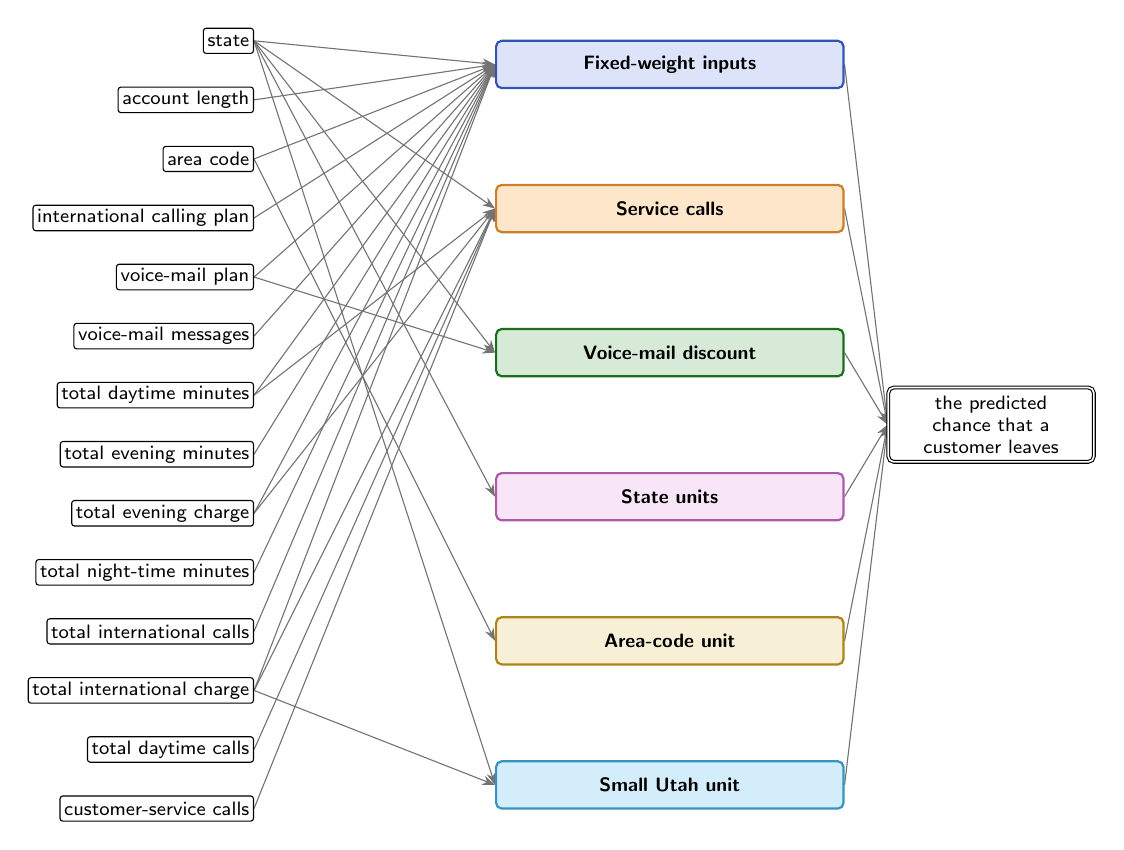
\begin{tikzpicture}[
  font=\sffamily\scriptsize, >={Stealth[length=1.6mm]},
  inp/.style={draw, rounded corners=1pt, fill=white, inner sep=1.5pt, minimum height=3.2mm, anchor=east},
  abox/.style={draw, thick, rounded corners=2pt, align=center, inner sep=3pt, minimum height=6mm, text width=42mm},
  outp/.style={draw, double, rounded corners=2pt, fill=white, align=center, inner sep=3pt, text width=24mm},
  agg/.style={draw=black!55},
]
\node[inp] (i0) at (0,4.875) {state};
\node[inp] (i1) at (0,4.125) {account length};
\node[inp] (i2) at (0,3.375) {area code};
\node[inp] (i3) at (0,2.625) {international calling plan};
\node[inp] (i4) at (0,1.875) {voice-mail plan};
\node[inp] (i5) at (0,1.125) {voice-mail messages};
\node[inp] (i6) at (0,0.375) {total daytime minutes};
\node[inp] (i7) at (0,-0.375) {total evening minutes};
\node[inp] (i8) at (0,-1.125) {total evening charge};
\node[inp] (i9) at (0,-1.875) {total night-time minutes};
\node[inp] (i10) at (0,-2.625) {total international calls};
\node[inp] (i11) at (0,-3.375) {total international charge};
\node[inp] (i12) at (0,-4.125) {total daytime calls};
\node[inp] (i13) at (0,-4.875) {customer-service calls};
\node[abox, fill=RoyalBlue!18, draw=RoyalBlue!80!black] (b0) at (5.28,4.575) {\textbf{Fixed-weight inputs}};
\node[abox, fill=BurntOrange!18, draw=BurntOrange!80!black] (b1) at (5.28,2.745) {\textbf{Service calls}};
\node[abox, fill=ForestGreen!18, draw=ForestGreen!80!black] (b2) at (5.28,0.915) {\textbf{Voice-mail discount}};
\node[abox, fill=Orchid!18, draw=Orchid!80!black] (b3) at (5.28,-0.915) {\textbf{State units}};
\node[abox, fill=Goldenrod!18, draw=Goldenrod!80!black] (b4) at (5.28,-2.745) {\textbf{Area-code unit}};
\node[abox, fill=Cerulean!18, draw=Cerulean!80!black] (b5) at (5.28,-4.575) {\textbf{Small Utah unit}};
\node[outp] (out) at (9.36,0) {the predicted chance that a customer leaves};
\begin{scope}[on background layer]
\draw[->, agg, thin] (i0.east) -- (b0.west);
\draw[->, agg, thin] (i1.east) -- (b0.west);
\draw[->, agg, thin] (i2.east) -- (b0.west);
\draw[->, agg, thin] (i3.east) -- (b0.west);
\draw[->, agg, thin] (i4.east) -- (b0.west);
\draw[->, agg, thin] (i5.east) -- (b0.west);
\draw[->, agg, thin] (i6.east) -- (b0.west);
\draw[->, agg, thin] (i7.east) -- (b0.west);
\draw[->, agg, thin] (i8.east) -- (b0.west);
\draw[->, agg, thin] (i9.east) -- (b0.west);
\draw[->, agg, thin] (i10.east) -- (b0.west);
\draw[->, agg, thin] (i11.east) -- (b0.west);
\draw[->, agg] (b0.east) -- (out.west);
\draw[->, agg, thin] (i0.east) -- (b1.west);
\draw[->, agg, thin] (i6.east) -- (b1.west);
\draw[->, agg, thin] (i12.east) -- (b1.west);
\draw[->, agg, thin] (i8.east) -- (b1.west);
\draw[->, agg, thin] (i11.east) -- (b1.west);
\draw[->, agg, thin] (i13.east) -- (b1.west);
\draw[->, agg] (b1.east) -- (out.west);
\draw[->, agg, thin] (i0.east) -- (b2.west);
\draw[->, agg, thin] (i4.east) -- (b2.west);
\draw[->, agg] (b2.east) -- (out.west);
\draw[->, agg, thin] (i0.east) -- (b3.west);
\draw[->, agg] (b3.east) -- (out.west);
\draw[->, agg, thin] (i2.east) -- (b4.west);
\draw[->, agg] (b4.east) -- (out.west);
\draw[->, agg, thin] (i0.east) -- (b5.west);
\draw[->, agg, thin] (i11.east) -- (b5.west);
\draw[->, agg] (b5.east) -- (out.west);
\end{scope}
\end{tikzpicture}}}%
\caption{The whole model: what feeds it, one level down.}
\label{fig:churn100s2c2:parts-ann97}
\end{figure}
\begin{figure}[H]\centering
\resizebox{\ifdim\width>\linewidth\linewidth\else\width\fi}{!}{%
\definecolor{netup}{HTML}{D95F02}\definecolor{netdown}{HTML}{1B9E77}\definecolor{netmixed}{HTML}{7F7F7F}%
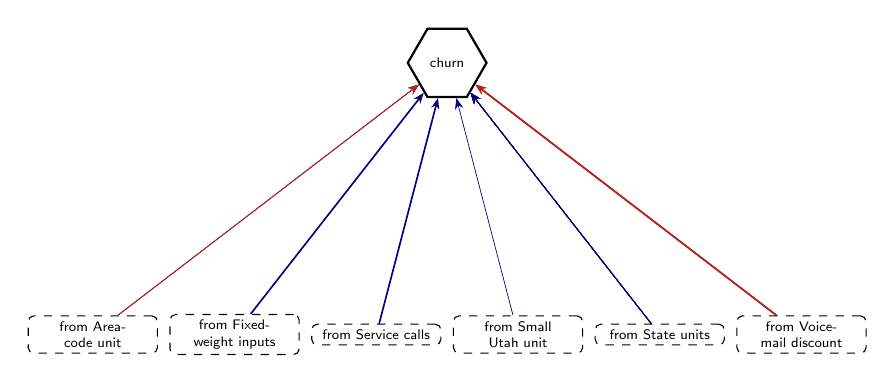
\begin{tikzpicture}[
  font=\sffamily\scriptsize, >={Stealth[length=1.4mm]},
  inp/.style={draw, circle, fill=white, minimum size=3.2mm, inner sep=0pt},
  hid/.style={draw, circle, fill=white, minimum size=5.2mm, inner sep=0.5pt, font=\sffamily\tiny},
  exitbox/.style={draw, thick, rectangle, fill=white, align=center, text width=17mm, minimum height=5mm, inner sep=1.5pt, font=\sffamily\tiny},
  sumbox/.style={draw, thick, dashed, rectangle, fill=white, align=center, text width=17mm, minimum height=5mm, inner sep=1.5pt, font=\sffamily\tiny},
  outp/.style={draw, thick, regular polygon, regular polygon sides=6, fill=white, minimum size=10mm, inner sep=0pt, font=\sffamily\tiny, align=center},
  stub/.style={draw, dashed, rounded corners=2pt, fill=white, align=center, inner sep=2pt, font=\sffamily\tiny, text width=15mm},
  inlab/.style={font=\sffamily\tiny, align=center, text width=15mm, inner sep=1pt, fill=white, fill opacity=0.8, text opacity=1},
  wpos/.style={draw=NavyBlue}, wneg/.style={draw=BrickRed}, wagg/.style={draw=black!45, line width=1.2pt},
  wmix/.style={draw=Plum},
]
\node[outp] (n0) at (5.4,3.45) {churn};
\node[stub] (nfromxxAreamcodexunit) at (0.9,0.0) {from Area-code unit};
\node[stub] (nfromxxSmallxUtahxunit) at (6.3,0.0) {from Small Utah unit};
\node[stub] (nfromxxVoicemmailxdiscount) at (9.9,0.0) {from Voice-mail discount};
\node[stub] (nfromxxStatexunits) at (8.1,0.0) {from State units};
\node[stub] (nfromxxFixedmweightxinputs) at (2.7,0.0) {from Fixed-weight inputs};
\node[stub] (nfromxxServicexcalls) at (4.5,0.0) {from Service calls};
\begin{scope}[on background layer]
\draw[->, wpos, line width=0.27pt] (nfromxxAreamcodexunit) -- (n0);
\draw[->, wpos, line width=0.25pt] (nfromxxSmallxUtahxunit) -- (n0);
\draw[->, wneg, line width=0.56pt] (nfromxxVoicemmailxdiscount) -- (n0);
\draw[->, wneg, line width=0.60pt] (nfromxxVoicemmailxdiscount) -- (n0);
\draw[->, wneg, line width=0.25pt] (nfromxxStatexunits) -- (n0);
\draw[->, wneg, line width=0.25pt] (nfromxxStatexunits) -- (n0);
\draw[->, wneg, line width=0.25pt] (nfromxxStatexunits) -- (n0);
\draw[->, wpos, line width=0.29pt] (nfromxxStatexunits) -- (n0);
\draw[->, wpos, line width=0.27pt] (nfromxxStatexunits) -- (n0);
\draw[->, wpos, line width=0.27pt] (nfromxxStatexunits) -- (n0);
\draw[->, wneg, line width=0.34pt] (nfromxxAreamcodexunit) -- (n0);
\draw[->, wpos, line width=0.27pt] (nfromxxStatexunits) -- (n0);
\draw[->, wpos, line width=0.27pt] (nfromxxStatexunits) -- (n0);
\draw[->, wpos, line width=0.60pt] (nfromxxFixedmweightxinputs) -- (n0);
\draw[->, wpos, line width=0.60pt] (nfromxxServicexcalls) -- (n0);
\end{scope}
\end{tikzpicture}}%
\caption{The whole model: its units and every connection into them. Blue: positive weight (raises the score); red: negative weight (lowers it); thicker: larger weight. Orange outline and up arrow: raises the final prediction; teal and down arrow: lowers it; grey and double arrow: depends.}
\label{fig:churn100s2c2:units-ann97}
\end{figure}
\paragraph{Hypothesis.} The model adds up six parts into one score: fixed-weight inputs, service calls, a voice-mail discount, state units, an area-code unit and a small Utah unit.\,{\scriptsize\textcolor{NavyBlue}{[C051]}}
\paragraph{Evidence.} It is made up of these six parts (each explained below); the score is their sum, which was checked on all 4000 training customers.\,{\scriptsize\textcolor{NavyBlue}{[C051]}} Changing one input at a time across the whole model, an international plan takes a typical customer's chance of leaving from about 1\% to about 14\%, and a voice-mail plan lowers it to under 1\%.\,{\scriptsize\textcolor{NavyBlue}{[C001, C010]}} In Washington the chance is about 9\%, against about 1\% in West Virginia.\,{\scriptsize\textcolor{NavyBlue}{[C003]}} More customer-service calls raise it slowly at first, then faster, from about 1\% at 0 calls to about 2\% at 3 calls.\,{\scriptsize\textcolor{NavyBlue}{[C011]}} The model ignores the daytime charge, evening calls, international minutes, night-time calls and the night-time charge.\,{\scriptsize\textcolor{NavyBlue}{[C046, C047, C048, C049, C050]}}
\par\noindent{\small Evidence plots: Figure~\ref{fig:churn100s2c2:plot-ann97-0}, Figure~\ref{fig:churn100s2c2:plot-ann97-1}.\par}
\begin{figure}[H]\centering
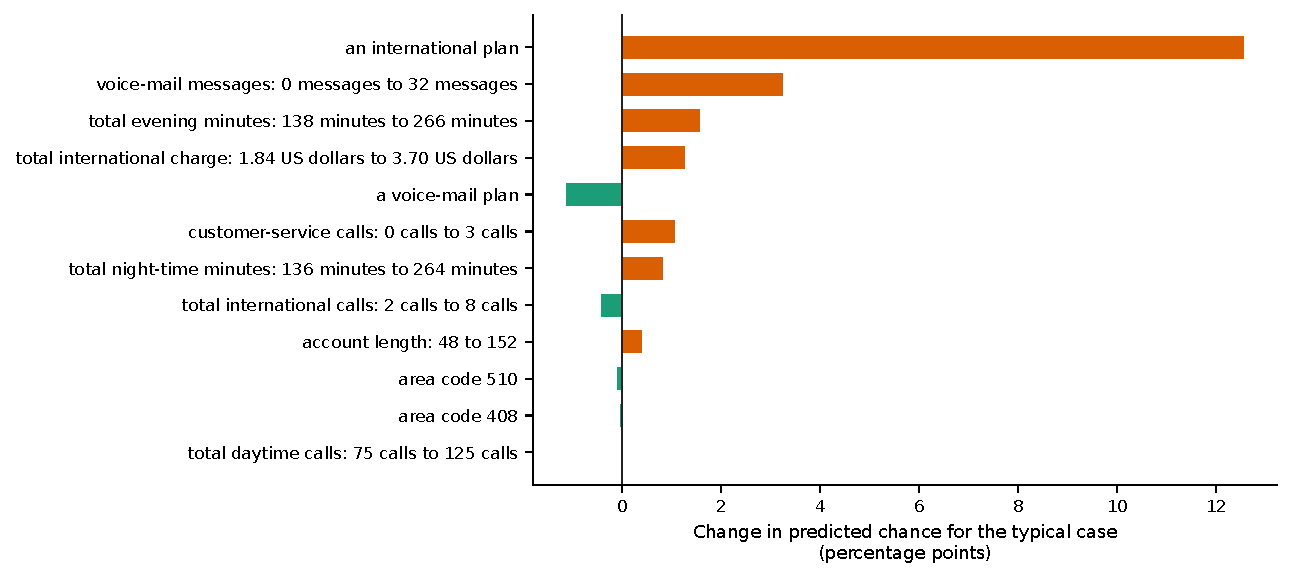
\includegraphics[width=\linewidth,height=0.88\textheight,keepaspectratio]{figures/churn100-s2-c2/ann_97-effects.pdf}
\caption{The whole model: Each input's change in the predicted value for the typical case across the whole model, largest first (orange: raises it, teal: lowers it).}
\label{fig:churn100s2c2:plot-ann97-0}
\end{figure}
\begin{figure}[H]\centering
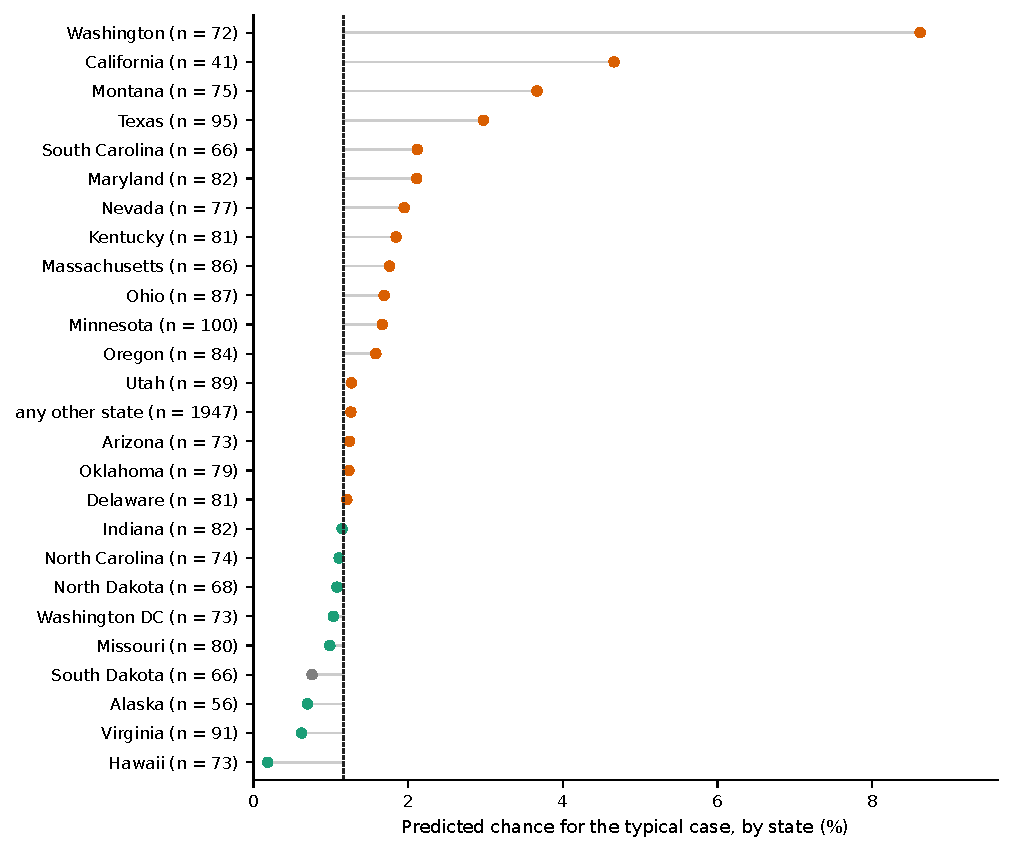
\includegraphics[width=\linewidth,height=0.88\textheight,keepaspectratio]{figures/churn100-s2-c2/ann_97-levels-state.pdf}
\caption{The whole model: Every level of state the model reads: the predicted value for the typical case at that level (dashed: the reference level); n = training customers; grey: few customers or not supported.}
\label{fig:churn100s2c2:plot-ann97-1}
\end{figure}
\par\smallskip\noindent{\small \textbf{Dive deeper:} Fixed-weight inputs (\ref{rd:ann89}); Service calls (\ref{rd:ann96}); Voice-mail discount (\ref{rd:ann92}); State units (\ref{rd:ann95}); Area-code unit (\ref{rd:ann94}); Small Utah unit (\ref{rd:ann93}). Technical detail: \ref{tech:ann97}.\par}
\subsubsection{Fixed-weight inputs}\label{rd:ann89}
\noindent{\footnotesize Part of: The whole model (\ref{rd:ann97}).\par}
\noindent{\small Figure~\ref{fig:churn100s2c2:parts-ann89} shows what feeds this part; Figure~\ref{fig:churn100s2c2:units-ann89} its units and every connection into them (dashed boxes: connections from or to other parts, drawn in their own sections).\par}
\begin{figure}[H]\centering
\resizebox{!}{\ifdim\height>0.5\textheight 0.5\textheight\else\height\fi}{%
\resizebox{\ifdim\width>\linewidth\linewidth\else\width\fi}{!}{%
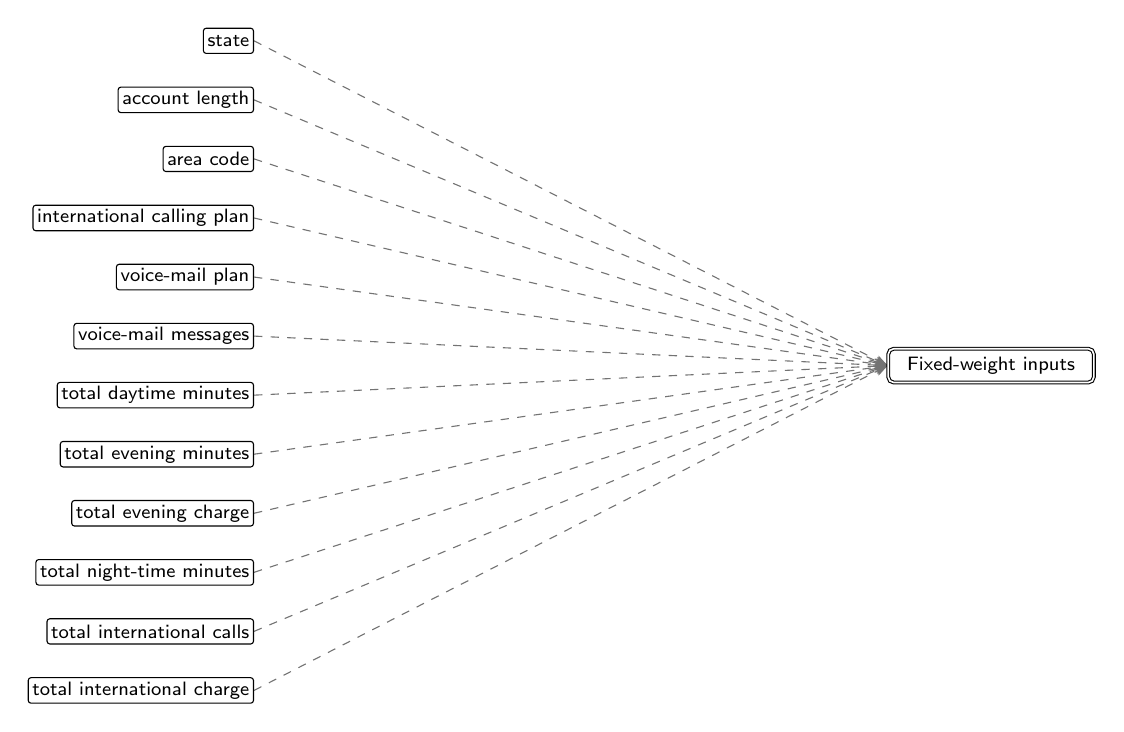
\begin{tikzpicture}[
  font=\sffamily\scriptsize, >={Stealth[length=1.6mm]},
  inp/.style={draw, rounded corners=1pt, fill=white, inner sep=1.5pt, minimum height=3.2mm, anchor=east},
  abox/.style={draw, thick, rounded corners=2pt, align=center, inner sep=3pt, minimum height=6mm, text width=42mm},
  outp/.style={draw, double, rounded corners=2pt, fill=white, align=center, inner sep=3pt, text width=24mm},
  agg/.style={draw=black!55},
]
\node[inp] (i0) at (0,4.125) {state};
\node[inp] (i1) at (0,3.375) {account length};
\node[inp] (i2) at (0,2.625) {area code};
\node[inp] (i3) at (0,1.875) {international calling plan};
\node[inp] (i4) at (0,1.125) {voice-mail plan};
\node[inp] (i5) at (0,0.375) {voice-mail messages};
\node[inp] (i6) at (0,-0.375) {total daytime minutes};
\node[inp] (i7) at (0,-1.125) {total evening minutes};
\node[inp] (i8) at (0,-1.875) {total evening charge};
\node[inp] (i9) at (0,-2.625) {total night-time minutes};
\node[inp] (i10) at (0,-3.375) {total international calls};
\node[inp] (i11) at (0,-4.125) {total international charge};
\node[outp] (out) at (9.36,0) {Fixed-weight inputs};
\begin{scope}[on background layer]
\draw[->, agg, thin, dashed] (i0.east) -- (out.west);
\draw[->, agg, thin, dashed] (i1.east) -- (out.west);
\draw[->, agg, thin, dashed] (i2.east) -- (out.west);
\draw[->, agg, thin, dashed] (i3.east) -- (out.west);
\draw[->, agg, thin, dashed] (i4.east) -- (out.west);
\draw[->, agg, thin, dashed] (i5.east) -- (out.west);
\draw[->, agg, thin, dashed] (i6.east) -- (out.west);
\draw[->, agg, thin, dashed] (i7.east) -- (out.west);
\draw[->, agg, thin, dashed] (i8.east) -- (out.west);
\draw[->, agg, thin, dashed] (i9.east) -- (out.west);
\draw[->, agg, thin, dashed] (i10.east) -- (out.west);
\draw[->, agg, thin, dashed] (i11.east) -- (out.west);
\end{scope}
\end{tikzpicture}}}%
\caption{Fixed-weight inputs: what feeds it, one level down.}
\label{fig:churn100s2c2:parts-ann89}
\end{figure}
\begin{figure}[H]\centering
\resizebox{\ifdim\width>\linewidth\linewidth\else\width\fi}{!}{%
\definecolor{netup}{HTML}{D95F02}\definecolor{netdown}{HTML}{1B9E77}\definecolor{netmixed}{HTML}{7F7F7F}%
\begin{tikzpicture}[
  font=\sffamily\scriptsize, >={Stealth[length=1.4mm]},
  inp/.style={draw, circle, fill=white, minimum size=3.2mm, inner sep=0pt},
  hid/.style={draw, circle, fill=white, minimum size=5.2mm, inner sep=0.5pt, font=\sffamily\tiny},
  exitbox/.style={draw, thick, rectangle, fill=white, align=center, text width=17mm, minimum height=5mm, inner sep=1.5pt, font=\sffamily\tiny},
  sumbox/.style={draw, thick, dashed, rectangle, fill=white, align=center, text width=17mm, minimum height=5mm, inner sep=1.5pt, font=\sffamily\tiny},
  outp/.style={draw, thick, regular polygon, regular polygon sides=6, fill=white, minimum size=10mm, inner sep=0pt, font=\sffamily\tiny, align=center},
  stub/.style={draw, dashed, rounded corners=2pt, fill=white, align=center, inner sep=2pt, font=\sffamily\tiny, text width=15mm},
  inlab/.style={font=\sffamily\tiny, align=center, text width=15mm, inner sep=1pt, fill=white, fill opacity=0.8, text opacity=1},
  wpos/.style={draw=NavyBlue}, wneg/.style={draw=BrickRed}, wagg/.style={draw=black!45, line width=1.2pt},
  wmix/.style={draw=Plum},
]
\node[exitbox] (nidentityxlin) at (5.85,1.9) {Fixed-weight inputs $\uparrow$};
\node[inp, draw=netmixed, very thick] (ngrpxxstate) at (4.5,0.0) {};
\path (ngrpxxstate.south) node[inlab, anchor=north] (labngrpxxstate) {state (26 of 51 used) $\updownarrow$};
\node[inp, draw=netup, very thick] (ninxxaccountxlength) at (1.8,-1.05) {};
\path (ninxxaccountxlength.south) node[inlab, anchor=north] (labninxxaccountxlength) {account length $\uparrow$};
\node[inp, draw=netdown, very thick] (ninxxareaxcodex510) at (3.6,-1.05) {};
\path (ninxxareaxcodex510.south) node[inlab, anchor=north] (labninxxareaxcodex510) {area code 510 $\downarrow$};
\node[inp, draw=netup, very thick] (ninxxinternationalxplan) at (2.7,0.0) {};
\path (ninxxinternationalxplan.south) node[inlab, anchor=north] (labninxxinternationalxplan) {an international plan $\uparrow$};
\node[inp, draw=netup, very thick] (ninxxnumberxvmailxmessages) at (10.8,-1.05) {};
\path (ninxxnumberxvmailxmessages.south) node[inlab, anchor=north] (labninxxnumberxvmailxmessages) {voice-mail messages $\uparrow$};
\node[inp, draw=netup, very thick] (ninxxtotalxevexminutes) at (7.2,-1.05) {};
\path (ninxxtotalxevexminutes.south) node[inlab, anchor=north] (labninxxtotalxevexminutes) {total evening minutes $\uparrow$};
\node[inp, draw=netup, very thick] (ninxxtotalxnightxminutes) at (9.9,0.0) {};
\path (ninxxtotalxnightxminutes.south) node[inlab, anchor=north] (labninxxtotalxnightxminutes) {total night-time minutes $\uparrow$};
\node[inp, draw=netdown, very thick] (ninxxtotalxintlxcalls) at (8.1,0.0) {};
\path (ninxxtotalxintlxcalls.south) node[inlab, anchor=north] (labninxxtotalxintlxcalls) {total international calls $\downarrow$};
\node[inp, draw=netup, very thick] (ninxxtotalxintlxcharge) at (9.0,-1.05) {};
\path (ninxxtotalxintlxcharge.south) node[inlab, anchor=north] (labninxxtotalxintlxcharge) {total international charge $\uparrow$};
\node[inp, draw=netup, very thick] (ninxxtotalxevexcharge) at (6.3,0.0) {};
\path (ninxxtotalxevexcharge.south) node[inlab, anchor=north] (labninxxtotalxevexcharge) {total evening charge $\uparrow$};
\node[inp, draw=netup, very thick] (ninxxtotalxdayxminutes) at (5.4,-1.05) {};
\path (ninxxtotalxdayxminutes.south) node[inlab, anchor=north] (labninxxtotalxdayxminutes) {total daytime minutes $\uparrow$};
\node[inp, draw=netdown, very thick] (ninxxvoicexmailxplan) at (0.9,0.0) {};
\path (ninxxvoicexmailxplan.south) node[inlab, anchor=north] (labninxxvoicexmailxplan) {a voice-mail plan $\downarrow$};
\node[stub] (ntoxxthexmodelxoutput) at (5.85,3.45) {to the model output};
\begin{scope}[on background layer]
\node[fit=(nidentityxlin) , inner sep=8pt, rounded corners=5pt, fill=BurntOrange!10, draw=BurntOrange!45] (clu0) {};
\draw[->, wpos, line width=0.29pt] (ninxxaccountxlength) -- (nidentityxlin);
\draw[->, wneg, line width=0.26pt] (ninxxareaxcodex510) -- (nidentityxlin);
\draw[->, wpos, line width=0.52pt] (ninxxinternationalxplan) -- (nidentityxlin);
\draw[->, wpos, line width=0.45pt] (ninxxnumberxvmailxmessages) -- (nidentityxlin);
\draw[->, wpos, line width=0.42pt] (ninxxtotalxevexminutes) -- (nidentityxlin);
\draw[->, wpos, line width=0.35pt] (ninxxtotalxnightxminutes) -- (nidentityxlin);
\draw[->, wneg, line width=0.31pt] (ninxxtotalxintlxcalls) -- (nidentityxlin);
\draw[->, wpos, line width=0.49pt] (ninxxtotalxintlxcharge) -- (nidentityxlin);
\draw[->, wpos, line width=0.37pt] (ninxxtotalxevexcharge) -- (nidentityxlin);
\draw[->, wpos, line width=0.90pt] (ninxxtotalxdayxminutes) -- (nidentityxlin);
\draw[->, wneg, line width=0.56pt] (ninxxvoicexmailxplan) -- (nidentityxlin);
\draw[->, wpos, line width=0.60pt] (nidentityxlin) -- (ntoxxthexmodelxoutput);
\draw[->, wmix, line width=0.34pt] (ngrpxxstate) -- node[pos=0.8, sloped, above, font=\sffamily\tiny, inner sep=1pt, fill=white, fill opacity=0.8, text opacity=1] {22 edges, -0.26 to +0.18} (nidentityxlin);
\end{scope}
\node[font=\sffamily\scriptsize\bfseries, text=BurntOrange!55!black, anchor=south west, inner sep=1pt, fill=white, fill opacity=0.85, text opacity=1] at (clu0.north west) {Fixed-weight inputs};
\end{tikzpicture}}%
\caption{Fixed-weight inputs: its units and every connection into them. Blue: positive weight (raises the score); red: negative weight (lowers it); thicker: larger weight. Orange outline and up arrow: raises the final prediction; teal and down arrow: lowers it; grey and double arrow: depends.}
\label{fig:churn100s2c2:units-ann89}
\end{figure}
\paragraph{Hypothesis.} This part adds up most inputs with fixed weights: daytime minutes, an international plan and voice-mail messages raise the chance of leaving, steadily for the minutes and messages, and a voice-mail plan lowers it.\,{\scriptsize\textcolor{NavyBlue}{[C053, C052, C056, C061]}}
\paragraph{Evidence.} Through it, daytime minutes take a typical customer steadily from under 1\% at 112 to about 11\% at 249 minutes, and an international plan from about 1\% to about 14\%; a voice-mail plan lowers the chance to under 1\%.\,{\scriptsize\textcolor{NavyBlue}{[C053, C052, C061]}} Through it, the state moves the chance from about 1\% in West Virginia to about 5\% in Washington and in California, and to under 1\% in Hawaii (41 to 122 training customers per state).\,{\scriptsize\textcolor{NavyBlue}{[C054, C055, C062]}} Its formula reproduces the part exactly on all 4000 training customers.\,{\scriptsize\textcolor{NavyBlue}{[C085]}}
\par\noindent{\small Evidence plots: Figure~\ref{fig:churn100s2c2:plot-ann89-0}, Figure~\ref{fig:churn100s2c2:plot-ann89-1}, Figure~\ref{fig:churn100s2c2:plot-ann89-2}, Figure~\ref{fig:churn100s2c2:plot-ann89-3}.\par}
\begin{figure}[H]\centering
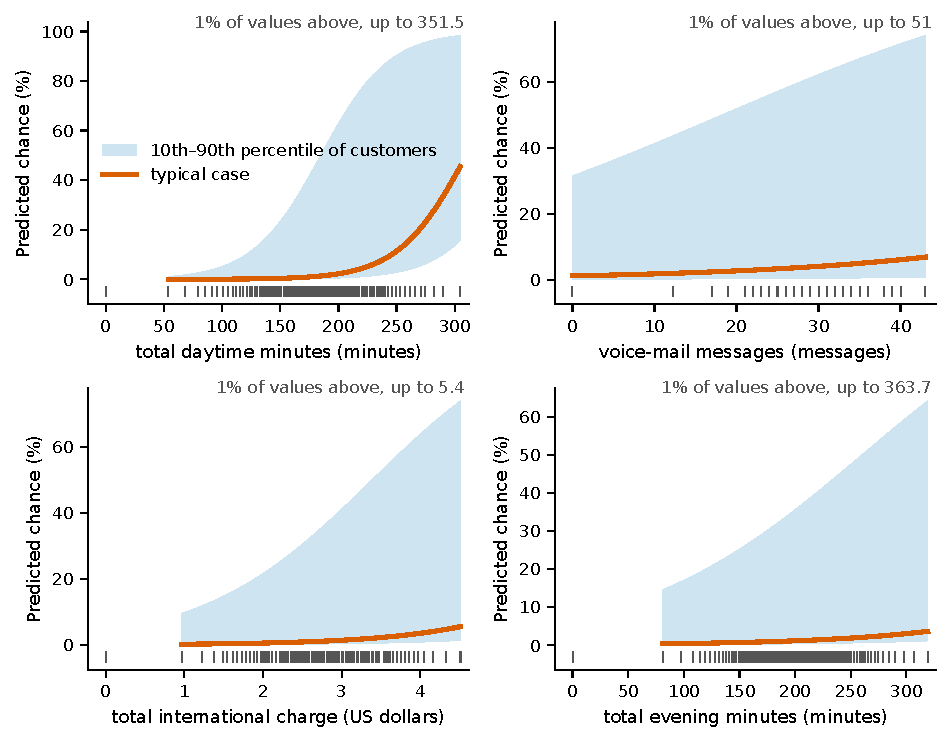
\includegraphics[width=\linewidth,height=0.88\textheight,keepaspectratio]{figures/churn100-s2-c2/ann_89-response.pdf}
\caption{Fixed-weight inputs: Response curves through this part: the typical case (bold), the 10th to 90th percentile of individual customers (band), the fold or step point (dashed) with its spread across them (grey), and the observed values (ticks).}
\label{fig:churn100s2c2:plot-ann89-0}
\end{figure}
\begin{figure}[H]\centering
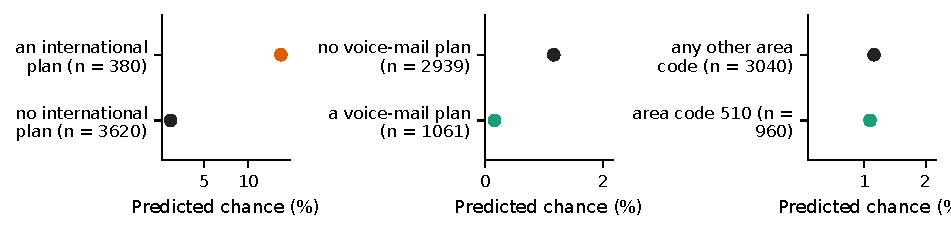
\includegraphics[width=\linewidth,height=0.88\textheight,keepaspectratio]{figures/churn100-s2-c2/ann_89-categories-small.pdf}
\caption{Fixed-weight inputs: The predicted value for the typical case at each level, through this part (n = training customers; grey: fewer than 20).}
\label{fig:churn100s2c2:plot-ann89-1}
\end{figure}
\begin{figure}[H]\centering
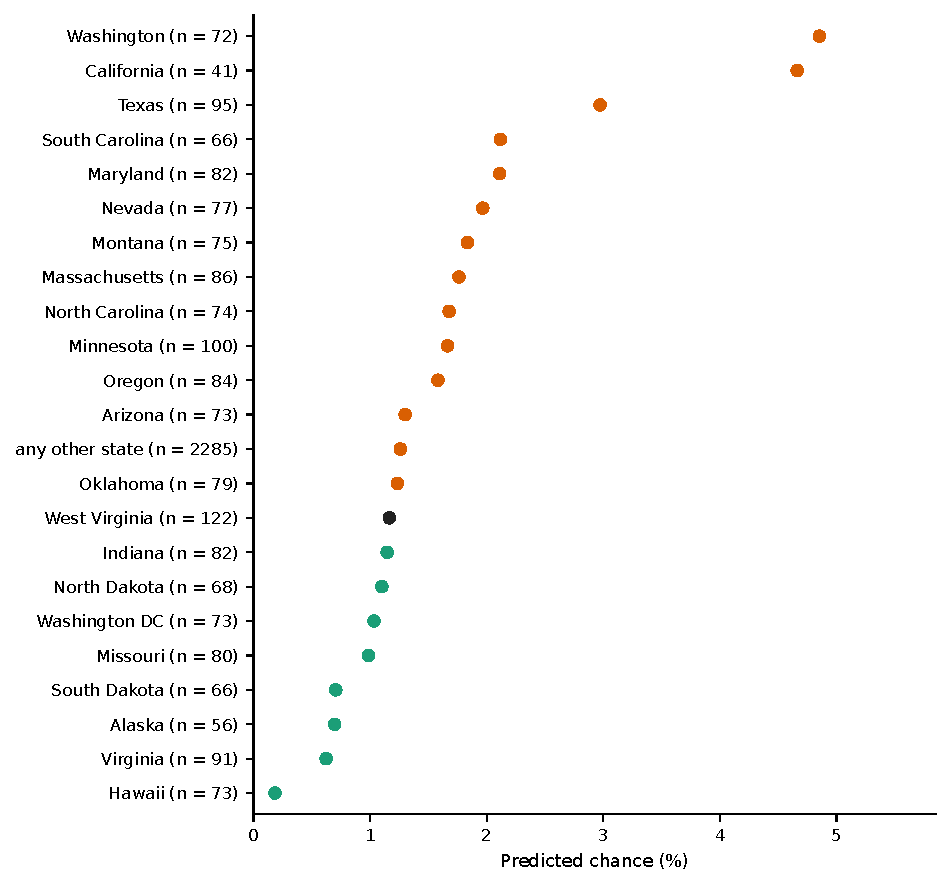
\includegraphics[width=\linewidth,height=0.88\textheight,keepaspectratio]{figures/churn100-s2-c2/ann_89-categories-C054.pdf}
\caption{Fixed-weight inputs: The predicted value for the typical case at each level, through this part (n = training customers; grey: fewer than 20).}
\label{fig:churn100s2c2:plot-ann89-2}
\end{figure}
\begin{figure}[H]\centering
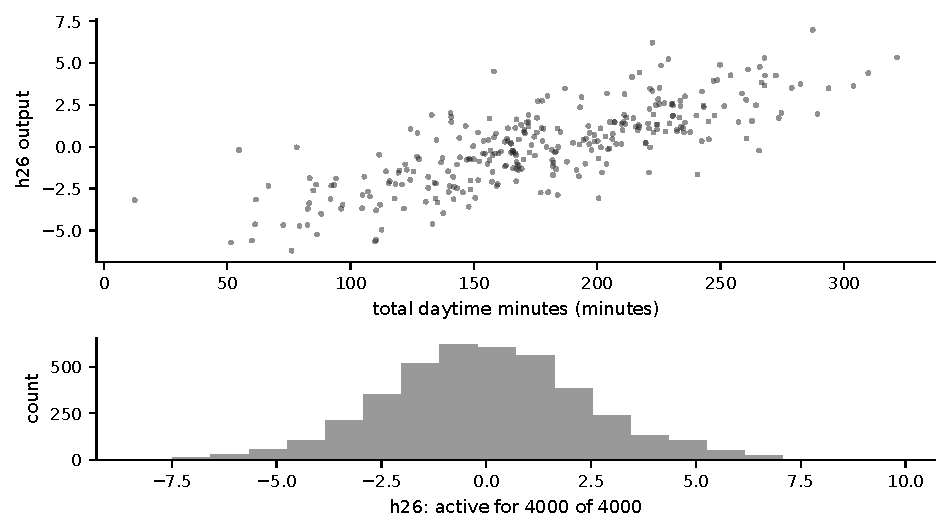
\includegraphics[width=\linewidth,height=0.88\textheight,keepaspectratio]{figures/churn100-s2-c2/ann_89-units.pdf}
\caption{Fixed-weight inputs: This part's hidden units: each unit's output against its main numeric input (top) and how often it is active (bottom).}
\label{fig:churn100s2c2:plot-ann89-3}
\end{figure}
\par\smallskip\noindent{\small Technical detail: \ref{tech:ann89}.\par}
\subsubsection{Service calls}\label{rd:ann96}
\noindent{\footnotesize Part of: The whole model (\ref{rd:ann97}).\par}
\noindent{\small Figure~\ref{fig:churn100s2c2:parts-ann96} shows what feeds this part; Figure~\ref{fig:churn100s2c2:units-ann96} its units and every connection into them (dashed boxes: connections from or to other parts, drawn in their own sections).\par}
\begin{figure}[H]\centering
\resizebox{!}{\ifdim\height>0.5\textheight 0.5\textheight\else\height\fi}{%
\resizebox{\ifdim\width>\linewidth\linewidth\else\width\fi}{!}{%
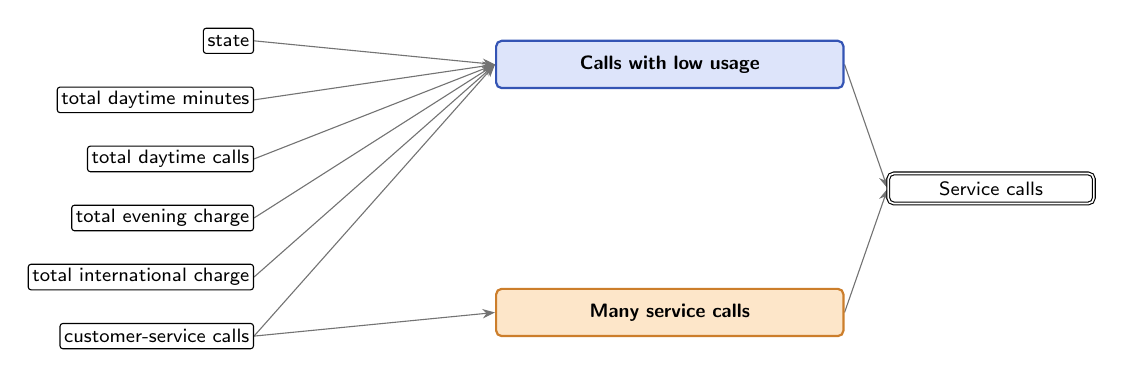
\begin{tikzpicture}[
  font=\sffamily\scriptsize, >={Stealth[length=1.6mm]},
  inp/.style={draw, rounded corners=1pt, fill=white, inner sep=1.5pt, minimum height=3.2mm, anchor=east},
  abox/.style={draw, thick, rounded corners=2pt, align=center, inner sep=3pt, minimum height=6mm, text width=42mm},
  outp/.style={draw, double, rounded corners=2pt, fill=white, align=center, inner sep=3pt, text width=24mm},
  agg/.style={draw=black!55},
]
\node[inp] (i0) at (0,1.875) {state};
\node[inp] (i1) at (0,1.125) {total daytime minutes};
\node[inp] (i2) at (0,0.375) {total daytime calls};
\node[inp] (i3) at (0,-0.375) {total evening charge};
\node[inp] (i4) at (0,-1.125) {total international charge};
\node[inp] (i5) at (0,-1.875) {customer-service calls};
\node[abox, fill=RoyalBlue!18, draw=RoyalBlue!80!black] (b0) at (5.28,1.575) {\textbf{Calls with low usage}};
\node[abox, fill=BurntOrange!18, draw=BurntOrange!80!black] (b1) at (5.28,-1.575) {\textbf{Many service calls}};
\node[outp] (out) at (9.36,0) {Service calls};
\begin{scope}[on background layer]
\draw[->, agg, thin] (i0.east) -- (b0.west);
\draw[->, agg, thin] (i1.east) -- (b0.west);
\draw[->, agg, thin] (i2.east) -- (b0.west);
\draw[->, agg, thin] (i3.east) -- (b0.west);
\draw[->, agg, thin] (i4.east) -- (b0.west);
\draw[->, agg, thin] (i5.east) -- (b0.west);
\draw[->, agg] (b0.east) -- (out.west);
\draw[->, agg, thin] (i5.east) -- (b1.west);
\draw[->, agg] (b1.east) -- (out.west);
\end{scope}
\end{tikzpicture}}}%
\caption{Service calls: what feeds it, one level down.}
\label{fig:churn100s2c2:parts-ann96}
\end{figure}
\begin{figure}[H]\centering
\resizebox{\ifdim\width>\linewidth\linewidth\else\width\fi}{!}{%
\definecolor{netup}{HTML}{D95F02}\definecolor{netdown}{HTML}{1B9E77}\definecolor{netmixed}{HTML}{7F7F7F}%
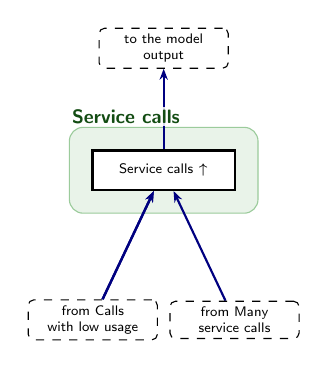
\begin{tikzpicture}[
  font=\sffamily\scriptsize, >={Stealth[length=1.4mm]},
  inp/.style={draw, circle, fill=white, minimum size=3.2mm, inner sep=0pt},
  hid/.style={draw, circle, fill=white, minimum size=5.2mm, inner sep=0.5pt, font=\sffamily\tiny},
  exitbox/.style={draw, thick, rectangle, fill=white, align=center, text width=17mm, minimum height=5mm, inner sep=1.5pt, font=\sffamily\tiny},
  sumbox/.style={draw, thick, dashed, rectangle, fill=white, align=center, text width=17mm, minimum height=5mm, inner sep=1.5pt, font=\sffamily\tiny},
  outp/.style={draw, thick, regular polygon, regular polygon sides=6, fill=white, minimum size=10mm, inner sep=0pt, font=\sffamily\tiny, align=center},
  stub/.style={draw, dashed, rounded corners=2pt, fill=white, align=center, inner sep=2pt, font=\sffamily\tiny, text width=15mm},
  inlab/.style={font=\sffamily\tiny, align=center, text width=15mm, inner sep=1pt, fill=white, fill opacity=0.8, text opacity=1},
  wpos/.style={draw=NavyBlue}, wneg/.style={draw=BrickRed}, wagg/.style={draw=black!45, line width=1.2pt},
  wmix/.style={draw=Plum},
]
\node[exitbox] (nidentityxsvc) at (1.8,1.9) {Service calls $\uparrow$};
\node[stub] (nfromxxCallsxwithxlowxusage) at (0.9,0.0) {from Calls with low usage};
\node[stub] (nfromxxManyxservicexcalls) at (2.7,0.0) {from Many service calls};
\node[stub] (ntoxxthexmodelxoutput) at (1.8,3.45) {to the model output};
\begin{scope}[on background layer]
\node[fit=(nidentityxsvc) , inner sep=8pt, rounded corners=5pt, fill=ForestGreen!10, draw=ForestGreen!45] (clu0) {};
\draw[->, wpos, line width=0.80pt] (nfromxxCallsxwithxlowxusage) -- (nidentityxsvc);
\draw[->, wpos, line width=0.88pt] (nfromxxCallsxwithxlowxusage) -- (nidentityxsvc);
\draw[->, wpos, line width=0.78pt] (nfromxxManyxservicexcalls) -- (nidentityxsvc);
\draw[->, wpos, line width=0.60pt] (nidentityxsvc) -- (ntoxxthexmodelxoutput);
\end{scope}
\node[font=\sffamily\scriptsize\bfseries, text=ForestGreen!55!black, anchor=south west, inner sep=1pt, fill=white, fill opacity=0.85, text opacity=1] at (clu0.north west) {Service calls};
\end{tikzpicture}}%
\caption{Service calls: its units and every connection into them. Blue: positive weight (raises the score); red: negative weight (lowers it); thicker: larger weight. Orange outline and up arrow: raises the final prediction; teal and down arrow: lowers it; grey and double arrow: depends.}
\label{fig:churn100s2c2:units-ann96}
\end{figure}
\paragraph{Hypothesis.} This part raises the chance of leaving with calls to customer service, from 4 calls upwards, slowly at first, then faster, and more so for customers with low daytime use, in an uneven way; it adds up two parts.\,{\scriptsize\textcolor{NavyBlue}{[C103, C099, C098]}}
\paragraph{Evidence.} It is made of two parts that are added: calls with low usage, and many service calls.\,{\scriptsize\textcolor{NavyBlue}{[C103]}} Through it, daytime minutes lower the chance only while they stay below about 166 minutes (between 145 and 213 minutes for different customers), in an uneven way: for a typical such customer, from about 28\% at 91 minutes to about 1\% at 352 minutes.\,{\scriptsize\textcolor{NavyBlue}{[C098]}} Customer-service calls add to it from 4 calls upwards, slowly at first, then faster: for a typical such customer, from about 3\% at 0 calls to about 8\% at 4 calls.\,{\scriptsize\textcolor{NavyBlue}{[C099]}} With an evening charge above 17.12 US dollars, the chance is lowest at about 148 minutes of daytime use and higher either side: from about 1\% at 112 minutes to about 13\% at 249 minutes, against about 2\% to about 9\% at or below that charge.\,{\scriptsize\textcolor{NavyBlue}{[C095]}}
\par\noindent{\small Evidence plots: Figure~\ref{fig:churn100s2c2:plot-ann96-0}, Figure~\ref{fig:churn100s2c2:plot-ann96-1}, Figure~\ref{fig:churn100s2c2:plot-ann96-2}, Figure~\ref{fig:churn100s2c2:plot-ann96-3}, Figure~\ref{fig:churn100s2c2:plot-ann96-4}, Figure~\ref{fig:churn100s2c2:plot-ann96-5}, Figure~\ref{fig:churn100s2c2:plot-ann96-6}, Figure~\ref{fig:churn100s2c2:plot-ann96-7}.\par}
\par\noindent{\small Figure~\ref{fig:churn100s2c2:plot-ann96-6} shows this part's own output, unit h27: over its two main inputs, with the line where it switches on.\par}
\begin{figure}[H]\centering
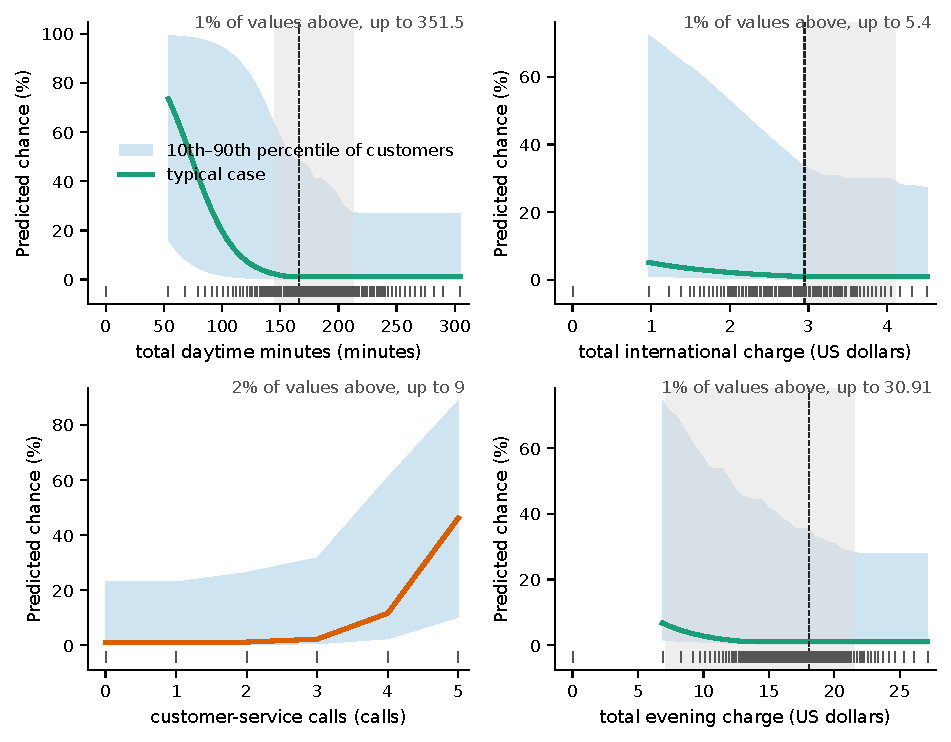
\includegraphics[width=\linewidth,height=0.88\textheight,keepaspectratio]{figures/churn100-s2-c2/ann_96-response.pdf}
\caption{Service calls: Response curves through this part: the typical case (bold), the 10th to 90th percentile of individual customers (band), the fold or step point (dashed) with its spread across them (grey), and the observed values (ticks).}
\label{fig:churn100s2c2:plot-ann96-0}
\end{figure}
\begin{figure}[H]\centering
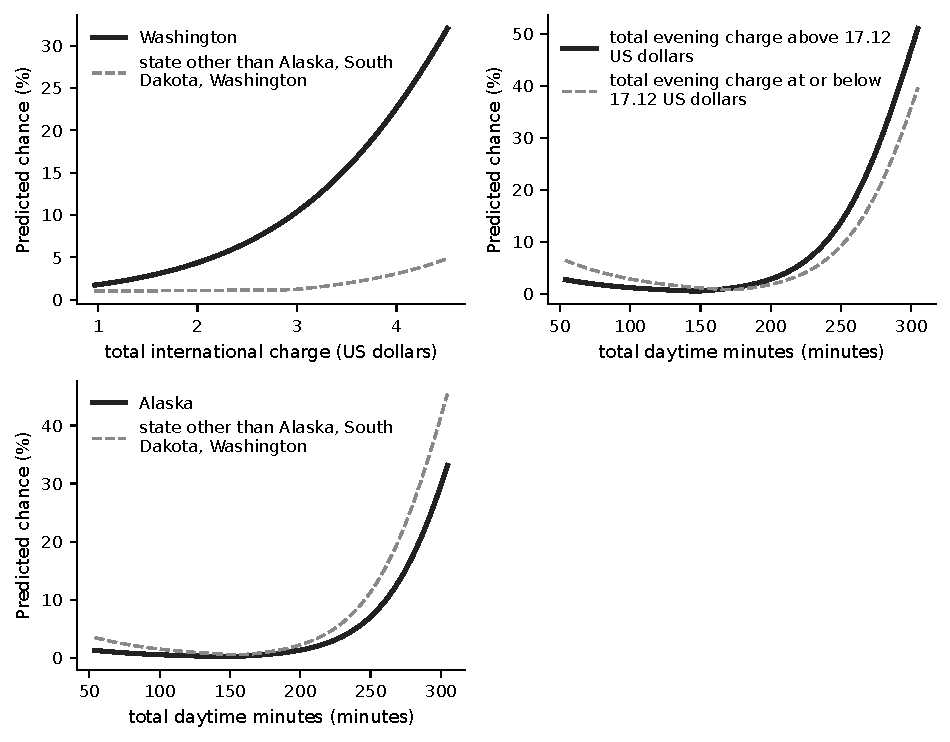
\includegraphics[width=\linewidth,height=0.88\textheight,keepaspectratio]{figures/churn100-s2-c2/ann_96-interaction.pdf}
\caption{Service calls: How the effect differs between groups: one curve per group, for the typical case of each group.}
\label{fig:churn100s2c2:plot-ann96-1}
\end{figure}
\begin{figure}[H]\centering
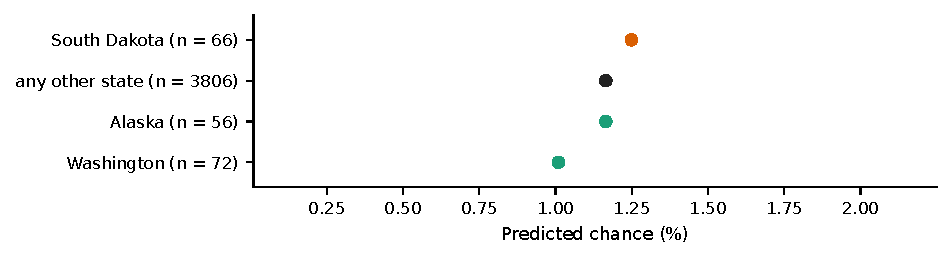
\includegraphics[width=\linewidth,height=0.88\textheight,keepaspectratio]{figures/churn100-s2-c2/ann_96-categories-small.pdf}
\caption{Service calls: The predicted value for the typical case at each level, through this part (n = training customers; grey: fewer than 20).}
\label{fig:churn100s2c2:plot-ann96-2}
\end{figure}
\begin{figure}[H]\centering
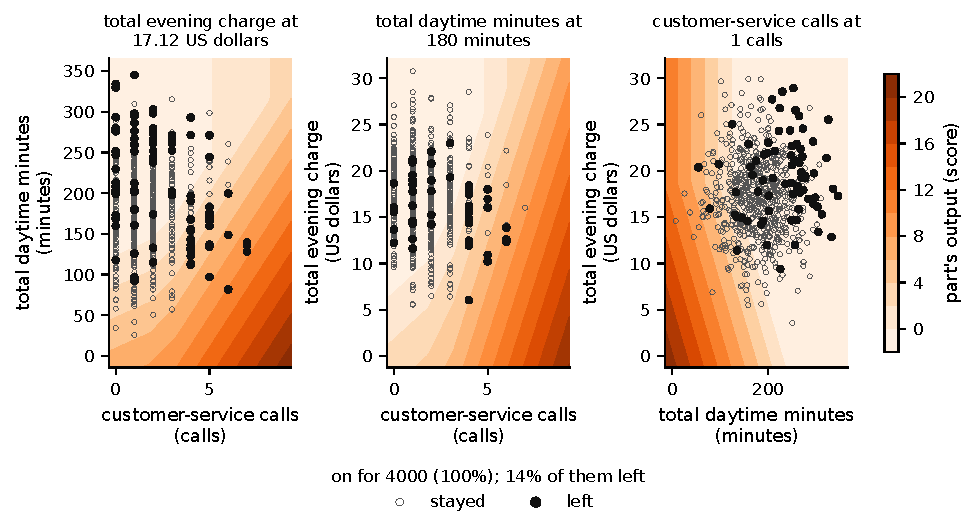
\includegraphics[width=\linewidth,height=0.88\textheight,keepaspectratio]{figures/churn100-s2-c2/ann_96-deep-map.pdf}
\caption{Service calls: The part's own output over each pair of its three main inputs (the third held at its median, named above each panel; the points are the training rows whose third input is between its 40th and 60th percentile), other inputs at the typical case: colour where it is on, flat grey where it is switched off, the black line where it switches on; training customers as hollow (no event) and filled (event) points, so the part can be seen catching the events (the predicted-chance overlay was harder to read). The switch-on line is traced on this map only; the boundary claim (C146) did not pass its check on the data, so no rule is stated.}
\label{fig:churn100s2c2:plot-ann96-3}
\end{figure}
\begin{figure}[H]\centering
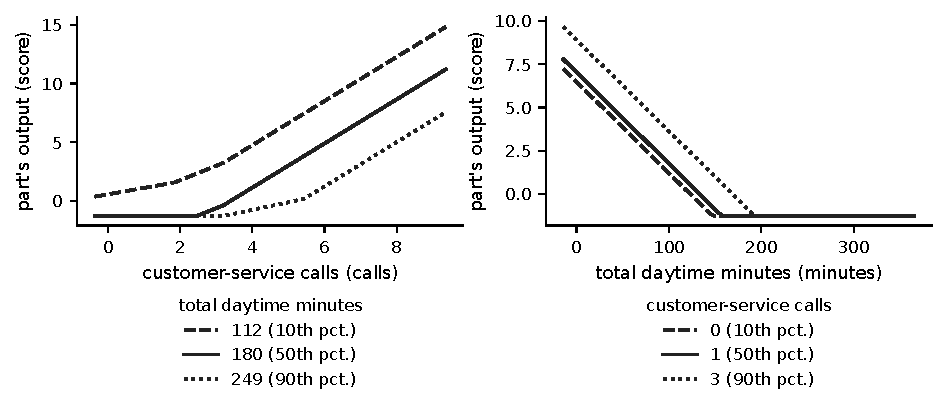
\includegraphics[width=\linewidth,height=0.88\textheight,keepaspectratio]{figures/churn100-s2-c2/ann_96-deep-slices.pdf}
\caption{Service calls: Slices of the same map: the part's own output against each input at three values of the other, so the tilted boundary shows as a shifting hinge. The switch-on line is traced on this map only; the boundary claim (C146) did not pass its check on the data, so no rule is stated.}
\label{fig:churn100s2c2:plot-ann96-4}
\end{figure}
\begin{figure}[H]\centering
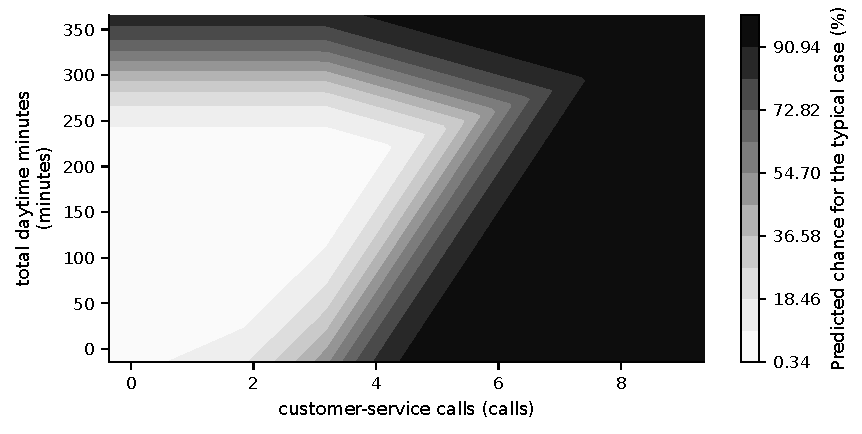
\includegraphics[width=\linewidth,height=0.88\textheight,keepaspectratio]{figures/churn100-s2-c2/ann_96-deep-risk.pdf}
\caption{Service calls: The same map on the final scale: the predicted value for the typical case, with the switch-on line (orange). The switch-on line is traced on this map only; the boundary claim (C146) did not pass its check on the data, so no rule is stated.}
\label{fig:churn100s2c2:plot-ann96-5}
\end{figure}
\begin{figure}[H]\centering
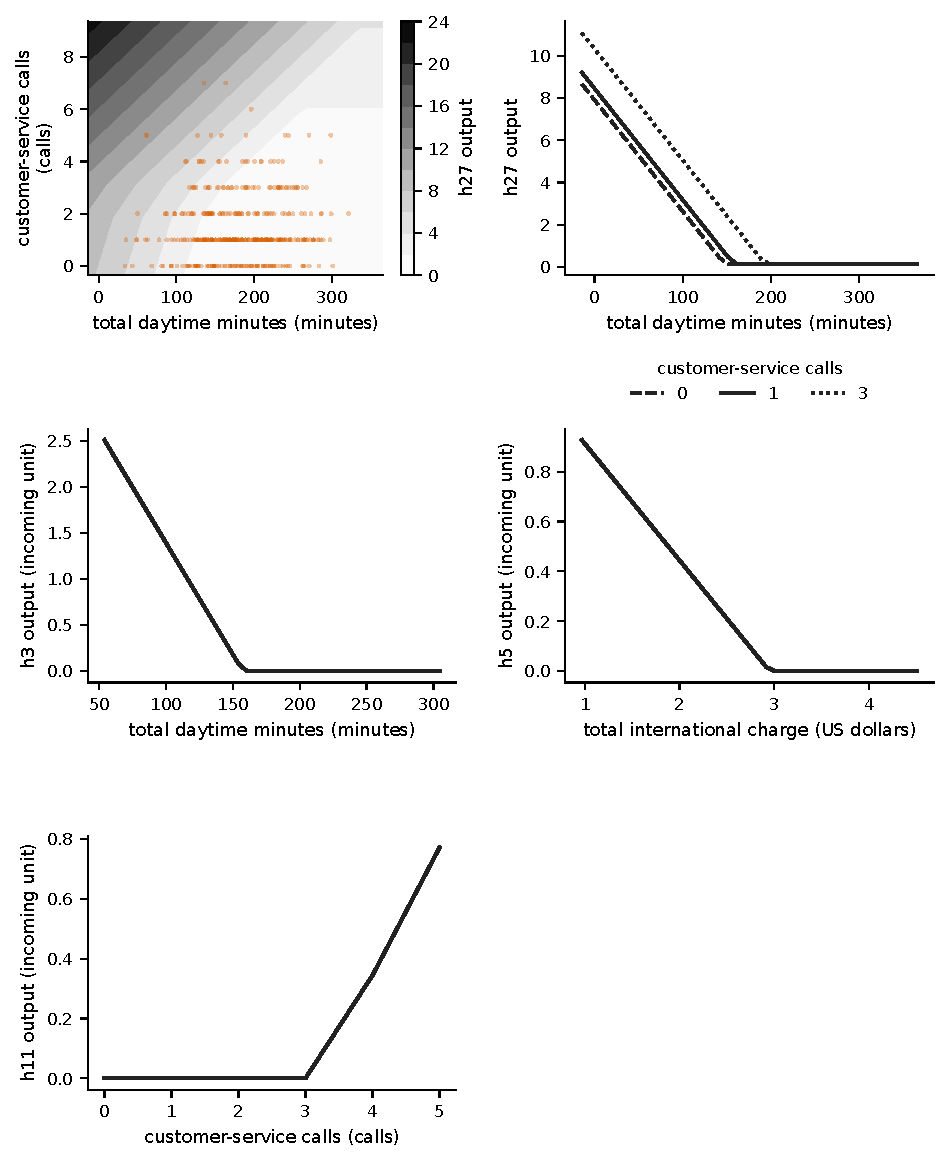
\includegraphics[width=\linewidth,height=0.88\textheight,keepaspectratio]{figures/churn100-s2-c2/ann_96-partial-identity_svc.pdf}
\caption{Service calls: This part's own output, unit h27 (combines 3 non-linear units), on its own scale (its activation), with every other input at the typical case; it is active for 3092 of 4000. Left: its output over its two main inputs (orange line: where it switches on; dots: the data); right: slices at three values of the second input; then each incoming non-linear unit against its own main input.}
\label{fig:churn100s2c2:plot-ann96-6}
\end{figure}
\begin{figure}[H]\centering
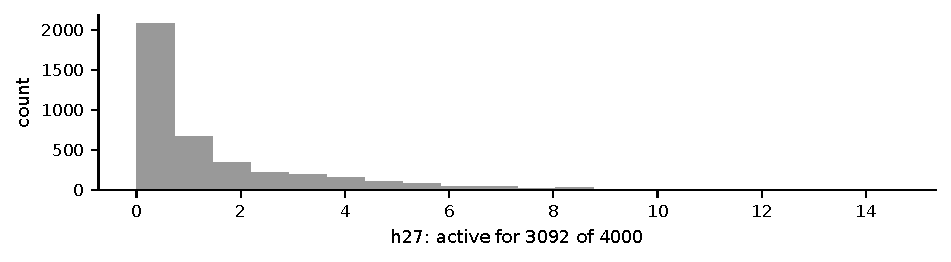
\includegraphics[width=\linewidth,height=0.88\textheight,keepaspectratio]{figures/churn100-s2-c2/ann_96-units.pdf}
\caption{Service calls: This part's hidden units: each unit's output against its main numeric input (top) and how often it is active (bottom).}
\label{fig:churn100s2c2:plot-ann96-7}
\end{figure}
\par\smallskip\noindent{\small \textbf{Dive deeper:} Calls with low usage (\ref{rd:ann90}); Many service calls (\ref{rd:ann91}). Technical detail: \ref{tech:ann96}.\par}
\subsubsection{Calls with low usage}\label{rd:ann90}
\noindent{\footnotesize Part of: Service calls (\ref{rd:ann96}).\par}
\noindent{\small Figure~\ref{fig:churn100s2c2:parts-ann90} shows what feeds this part; Figure~\ref{fig:churn100s2c2:units-ann90} its units and every connection into them (dashed boxes: connections from or to other parts, drawn in their own sections).\par}
\begin{figure}[H]\centering
\resizebox{!}{\ifdim\height>0.5\textheight 0.5\textheight\else\height\fi}{%
\resizebox{\ifdim\width>\linewidth\linewidth\else\width\fi}{!}{%
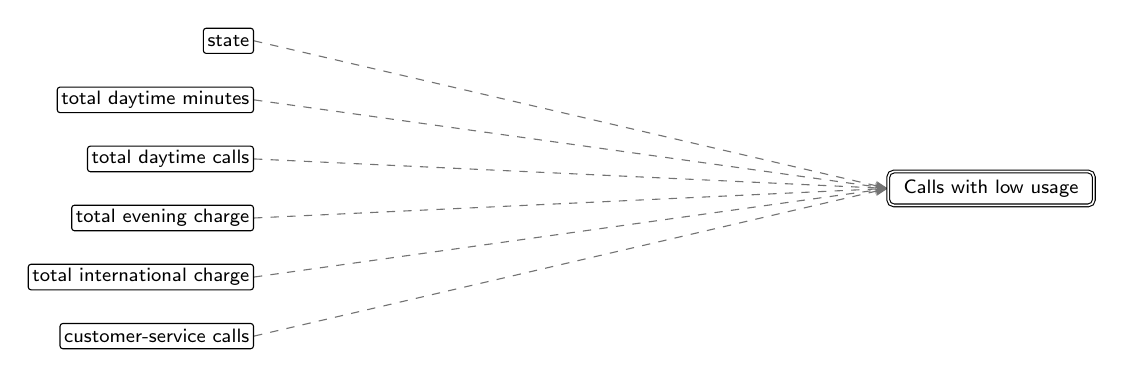
\begin{tikzpicture}[
  font=\sffamily\scriptsize, >={Stealth[length=1.6mm]},
  inp/.style={draw, rounded corners=1pt, fill=white, inner sep=1.5pt, minimum height=3.2mm, anchor=east},
  abox/.style={draw, thick, rounded corners=2pt, align=center, inner sep=3pt, minimum height=6mm, text width=42mm},
  outp/.style={draw, double, rounded corners=2pt, fill=white, align=center, inner sep=3pt, text width=24mm},
  agg/.style={draw=black!55},
]
\node[inp] (i0) at (0,1.875) {state};
\node[inp] (i1) at (0,1.125) {total daytime minutes};
\node[inp] (i2) at (0,0.375) {total daytime calls};
\node[inp] (i3) at (0,-0.375) {total evening charge};
\node[inp] (i4) at (0,-1.125) {total international charge};
\node[inp] (i5) at (0,-1.875) {customer-service calls};
\node[outp] (out) at (9.36,0) {Calls with low usage};
\begin{scope}[on background layer]
\draw[->, agg, thin, dashed] (i0.east) -- (out.west);
\draw[->, agg, thin, dashed] (i1.east) -- (out.west);
\draw[->, agg, thin, dashed] (i2.east) -- (out.west);
\draw[->, agg, thin, dashed] (i3.east) -- (out.west);
\draw[->, agg, thin, dashed] (i4.east) -- (out.west);
\draw[->, agg, thin, dashed] (i5.east) -- (out.west);
\end{scope}
\end{tikzpicture}}}%
\caption{Calls with low usage: what feeds it, one level down.}
\label{fig:churn100s2c2:parts-ann90}
\end{figure}
\begin{figure}[H]\centering
\resizebox{\ifdim\width>\linewidth\linewidth\else\width\fi}{!}{%
\definecolor{netup}{HTML}{D95F02}\definecolor{netdown}{HTML}{1B9E77}\definecolor{netmixed}{HTML}{7F7F7F}%
\begin{tikzpicture}[
  font=\sffamily\scriptsize, >={Stealth[length=1.4mm]},
  inp/.style={draw, circle, fill=white, minimum size=3.2mm, inner sep=0pt},
  hid/.style={draw, circle, fill=white, minimum size=5.2mm, inner sep=0.5pt, font=\sffamily\tiny},
  exitbox/.style={draw, thick, rectangle, fill=white, align=center, text width=17mm, minimum height=5mm, inner sep=1.5pt, font=\sffamily\tiny},
  sumbox/.style={draw, thick, dashed, rectangle, fill=white, align=center, text width=17mm, minimum height=5mm, inner sep=1.5pt, font=\sffamily\tiny},
  outp/.style={draw, thick, regular polygon, regular polygon sides=6, fill=white, minimum size=10mm, inner sep=0pt, font=\sffamily\tiny, align=center},
  stub/.style={draw, dashed, rounded corners=2pt, fill=white, align=center, inner sep=2pt, font=\sffamily\tiny, text width=15mm},
  inlab/.style={font=\sffamily\tiny, align=center, text width=15mm, inner sep=1pt, fill=white, fill opacity=0.8, text opacity=1},
  wpos/.style={draw=NavyBlue}, wneg/.style={draw=BrickRed}, wagg/.style={draw=black!45, line width=1.2pt},
  wmix/.style={draw=Plum},
]
\node[hid] (n15509) at (4.65,1.9) {h23};
\node[hid] (n2796) at (6.15,3.25) {h7};
\node[hid] (n807) at (5.4,4.6) {h3};
\node[hid] (n9555) at (6.15,1.9) {h15};
\node[hid] (n1264) at (5.4,5.95) {h5};
\node[hid] (n2627) at (4.65,3.25) {h6};
\node[inp, draw=netup, very thick] (ninxxtotalxdayxcalls) at (2.7,0.0) {};
\path (ninxxtotalxdayxcalls.south) node[inlab, anchor=north] (labninxxtotalxdayxcalls) {total daytime calls $\uparrow$};
\node[inp, draw=netdown, very thick] (ninxxtotalxintlxcharge) at (6.3,0.0) {};
\path (ninxxtotalxintlxcharge.south) node[inlab, anchor=north] (labninxxtotalxintlxcharge) {total international charge $\downarrow$};
\node[inp, draw=netdown, very thick] (ninxxtotalxevexcharge) at (9.9,0.0) {};
\path (ninxxtotalxevexcharge.south) node[inlab, anchor=north] (labninxxtotalxevexcharge) {total evening charge $\downarrow$};
\node[inp, draw=netdown, very thick] (ninxxtotalxdayxminutes) at (4.5,0.0) {};
\path (ninxxtotalxdayxminutes.south) node[inlab, anchor=north] (labninxxtotalxdayxminutes) {total daytime minutes $\downarrow$};
\node[inp, draw=netmixed, very thick] (ngrpxxstate) at (8.1,0.0) {};
\path (ngrpxxstate.south) node[inlab, anchor=north] (labngrpxxstate) {state (26 of 51 used) $\updownarrow$};
\node[inp, draw=netup, very thick] (ninxxnumberxcustomerxservicexcalls) at (0.9,0.0) {};
\path (ninxxnumberxcustomerxservicexcalls.south) node[inlab, anchor=north] (labninxxnumberxcustomerxservicexcalls) {customer-service calls $\uparrow$};
\node[stub] (ntoxxServicexcalls) at (5.4,7.5) {to Service calls};
\begin{scope}[on background layer]
\node[fit=(n15509) (n2796) (n807) (n9555) (n1264) (n2627) , inner sep=8pt, rounded corners=5pt, fill=ForestGreen!10, draw=ForestGreen!45] (clu0) {};
\draw[->, wpos, line width=0.27pt] (ninxxtotalxdayxcalls) -- (n807);
\draw[->, wpos, line width=0.46pt] (n2627) -- (n807);
\draw[->, wpos, line width=0.45pt] (n2796) -- (n807);
\draw[->, wpos, line width=0.37pt] (n807) -- (n1264);
\draw[->, wpos, line width=0.38pt] (n9555) -- (n2627);
\draw[->, wpos, line width=0.38pt] (n15509) -- (n2796);
\draw[->, wneg, line width=0.37pt] (ninxxtotalxintlxcharge) -- (n1264);
\draw[->, wneg, line width=0.60pt] (ninxxtotalxevexcharge) -- (n2796);
\draw[->, wneg, line width=0.71pt] (ninxxtotalxdayxminutes) -- (n807);
\draw[->, wpos, line width=0.33pt] (ninxxnumberxcustomerxservicexcalls) -- (n2627);
\draw[->, wpos, line width=0.36pt] (ninxxnumberxcustomerxservicexcalls) -- (n2796);
\draw[->, wpos, line width=0.57pt] (ninxxnumberxcustomerxservicexcalls) -- (n9555);
\draw[->, wpos, line width=0.60pt] (ninxxnumberxcustomerxservicexcalls) -- (n15509);
\draw[->, wpos, line width=0.80pt] (n807) -- (ntoxxServicexcalls);
\draw[->, wpos, line width=0.88pt] (n1264) -- (ntoxxServicexcalls);
\draw[->, wneg, line width=0.39pt] (ngrpxxstate) -- node[pos=0.8, sloped, above, font=\sffamily\tiny, inner sep=1pt, fill=white, fill opacity=0.8, text opacity=1] {-0.40} (n1264);
\draw[->, wmix, line width=0.74pt] (ngrpxxstate) -- node[pos=0.8, sloped, above, font=\sffamily\tiny, inner sep=1pt, fill=white, fill opacity=0.8, text opacity=1] {2 edges, -1.41 to +0.13} (n2796);
\end{scope}
\node[font=\sffamily\scriptsize\bfseries, text=ForestGreen!55!black, anchor=south west, inner sep=1pt, fill=white, fill opacity=0.85, text opacity=1] at (clu0.north west) {Calls with low usage};
\end{tikzpicture}}%
\caption{Calls with low usage: its units and every connection into them. Blue: positive weight (raises the score); red: negative weight (lowers it); thicker: larger weight. Orange outline and up arrow: raises the final prediction; teal and down arrow: lowers it; grey and double arrow: depends.}
\label{fig:churn100s2c2:units-ann90}
\end{figure}
\paragraph{Hypothesis.} This part raises the chance of leaving for customers with low usage, more so when they call customer service: daytime minutes lower it only while they stay below about 166 minutes (between 145 and 213 minutes for different customers), and calls raise it, both in an uneven way.\,{\scriptsize\textcolor{NavyBlue}{[C112, C106]}}
\paragraph{Evidence.} It acts on 3063 of 4000 training customers, 393 of whom left; for the typical customer it acts on, it changes the chance by less than a point.\,{\scriptsize\textcolor{NavyBlue}{[C117]}} Through it, a typical customer's chance falls in an uneven way from about 28\% at 91 minutes of daytime use to about 1\% at 352 minutes, with no further fall past about 166 minutes (between 145 and 213 minutes for different customers).\,{\scriptsize\textcolor{NavyBlue}{[C112]}} A higher international charge lowers it steadily up to about 2.95 US dollars (between 2.95 and 4.10 US dollars for different customers), then no further: for a typical such customer, from about 4\% to about 1\%.\,{\scriptsize\textcolor{NavyBlue}{[C115]}} Customer-service calls raise it in an uneven way, from about 1\% at 0 calls to about 2\% at 3 calls.\,{\scriptsize\textcolor{NavyBlue}{[C106]}} Its formula reproduces the part exactly on all 4000 training customers.\,{\scriptsize\textcolor{NavyBlue}{[C118]}}
\par\noindent{\small Evidence plots: Figure~\ref{fig:churn100s2c2:plot-ann90-0}, Figure~\ref{fig:churn100s2c2:plot-ann90-1}, Figure~\ref{fig:churn100s2c2:plot-ann90-2}, Figure~\ref{fig:churn100s2c2:plot-ann90-3}, Figure~\ref{fig:churn100s2c2:plot-ann90-4}, Figure~\ref{fig:churn100s2c2:plot-ann90-5}, Figure~\ref{fig:churn100s2c2:plot-ann90-6}, Figure~\ref{fig:churn100s2c2:plot-ann90-7}.\par}
\par\noindent{\small Figure~\ref{fig:churn100s2c2:plot-ann90-5} shows this part's own output, unit h3: over its two main inputs, with the line where it switches on.\par}
\par\noindent{\small Figure~\ref{fig:churn100s2c2:plot-ann90-6} shows this part's own output, unit h5: over its two main inputs, with the line where it switches on.\par}
\begin{figure}[H]\centering
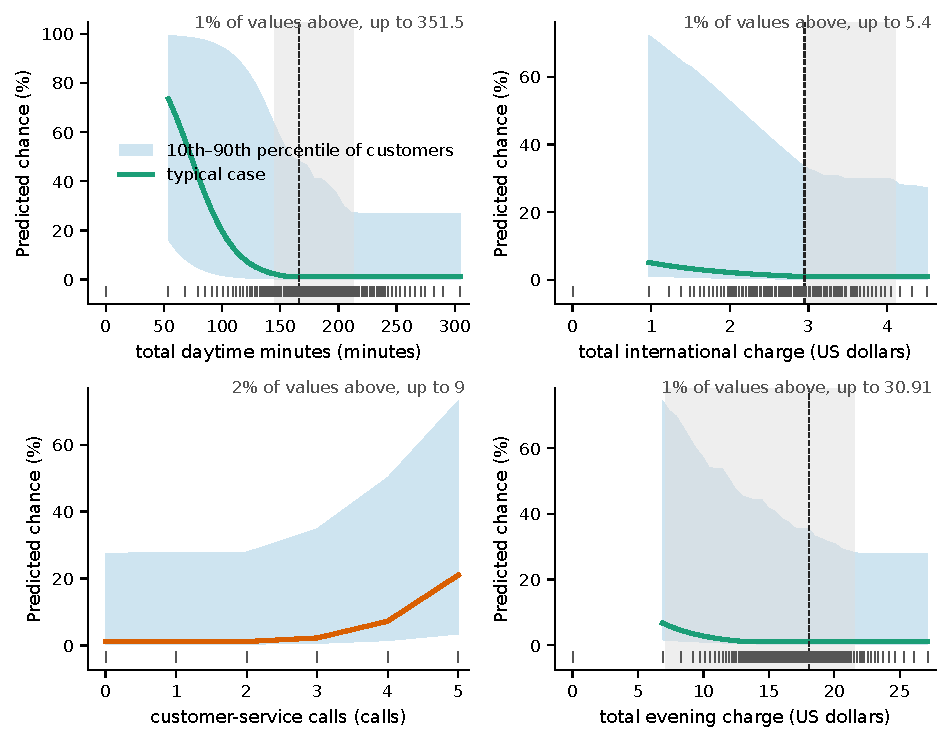
\includegraphics[width=\linewidth,height=0.88\textheight,keepaspectratio]{figures/churn100-s2-c2/ann_90-response.pdf}
\caption{Calls with low usage: Response curves through this part: the typical case (bold), the 10th to 90th percentile of individual customers (band), the fold or step point (dashed) with its spread across them (grey), and the observed values (ticks).}
\label{fig:churn100s2c2:plot-ann90-0}
\end{figure}
\begin{figure}[H]\centering
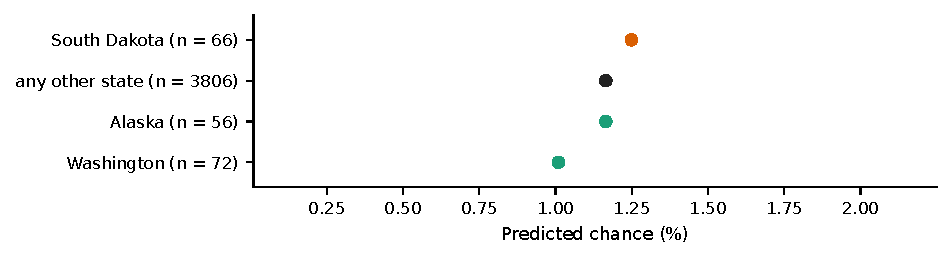
\includegraphics[width=\linewidth,height=0.88\textheight,keepaspectratio]{figures/churn100-s2-c2/ann_90-categories-small.pdf}
\caption{Calls with low usage: The predicted value for the typical case at each level, through this part (n = training customers; grey: fewer than 20).}
\label{fig:churn100s2c2:plot-ann90-1}
\end{figure}
\begin{figure}[H]\centering
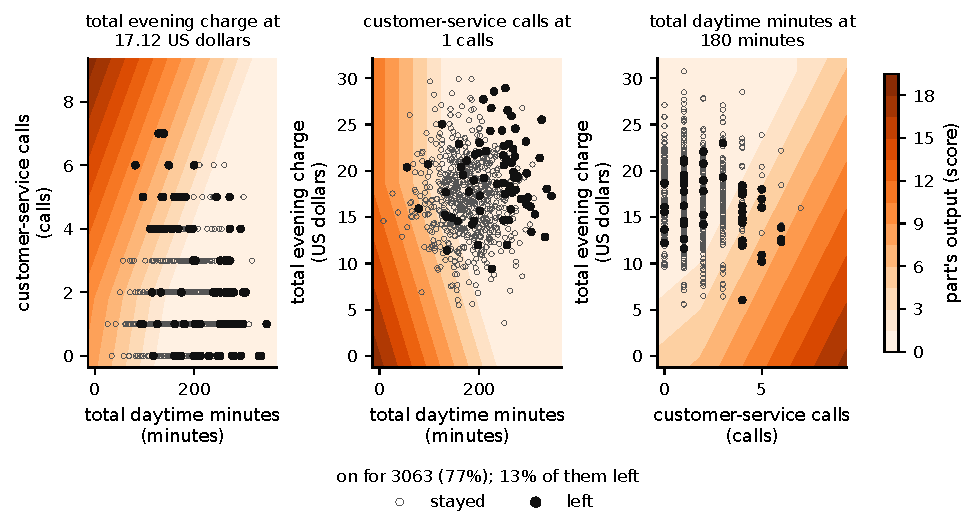
\includegraphics[width=\linewidth,height=0.88\textheight,keepaspectratio]{figures/churn100-s2-c2/ann_90-deep-map.pdf}
\caption{Calls with low usage: The part's own output over each pair of its three main inputs (the third held at its median, named above each panel; the points are the training rows whose third input is between its 40th and 60th percentile), other inputs at the typical case: colour where it is on, flat grey where it is switched off, the black line where it switches on; training customers as hollow (no event) and filled (event) points, so the part can be seen catching the events (the predicted-chance overlay was harder to read). The switch-on line is traced on this map only; the boundary claim (C147) did not pass its check on the data, so no rule is stated.}
\label{fig:churn100s2c2:plot-ann90-2}
\end{figure}
\begin{figure}[H]\centering
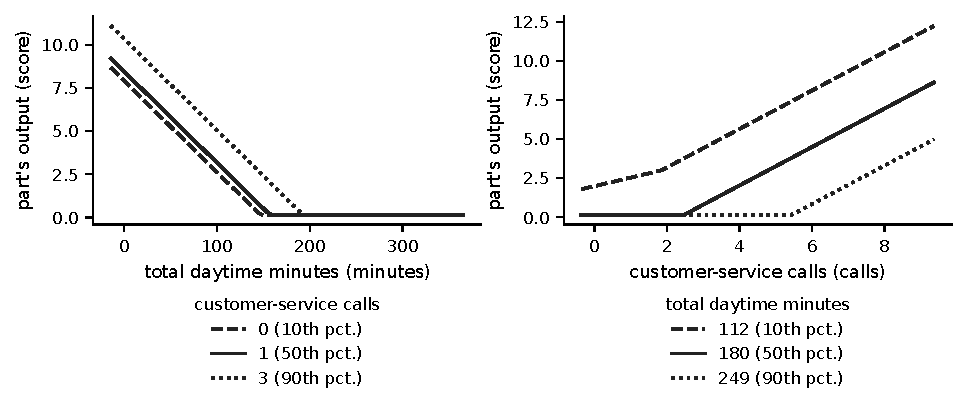
\includegraphics[width=\linewidth,height=0.88\textheight,keepaspectratio]{figures/churn100-s2-c2/ann_90-deep-slices.pdf}
\caption{Calls with low usage: Slices of the same map: the part's own output against each input at three values of the other, so the tilted boundary shows as a shifting hinge. The switch-on line is traced on this map only; the boundary claim (C147) did not pass its check on the data, so no rule is stated.}
\label{fig:churn100s2c2:plot-ann90-3}
\end{figure}
\begin{figure}[H]\centering
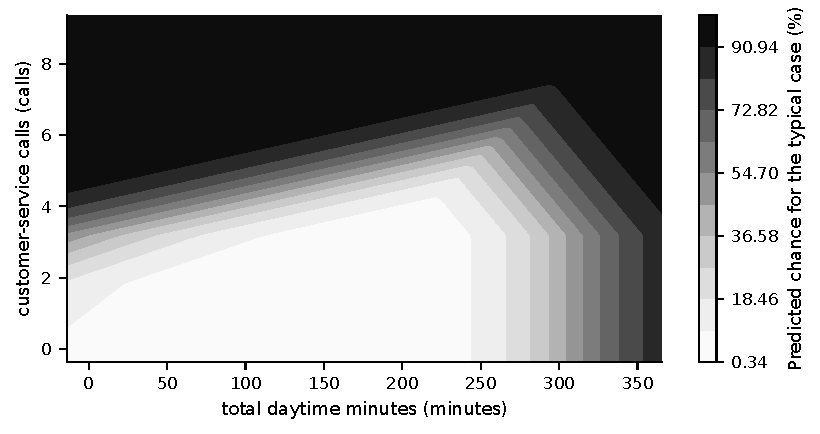
\includegraphics[width=\linewidth,height=0.88\textheight,keepaspectratio]{figures/churn100-s2-c2/ann_90-deep-risk.pdf}
\caption{Calls with low usage: The same map on the final scale: the predicted value for the typical case, with the switch-on line (orange). The switch-on line is traced on this map only; the boundary claim (C147) did not pass its check on the data, so no rule is stated.}
\label{fig:churn100s2c2:plot-ann90-4}
\end{figure}
\begin{figure}[H]\centering
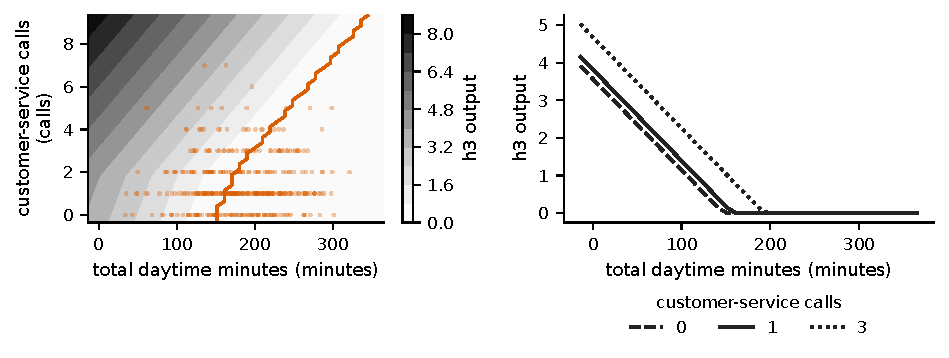
\includegraphics[width=\linewidth,height=0.88\textheight,keepaspectratio]{figures/churn100-s2-c2/ann_90-partial-807.pdf}
\caption{Calls with low usage: This part's own output, unit h3 (the output of 'Calls with low usage'), on its own scale (its activation), with every other input at the typical case; it is active for 1744 of 4000. Left: its output over its two main inputs (orange line: where it switches on; dots: the data); right: slices at three values of the second input.}
\label{fig:churn100s2c2:plot-ann90-5}
\end{figure}
\begin{figure}[H]\centering
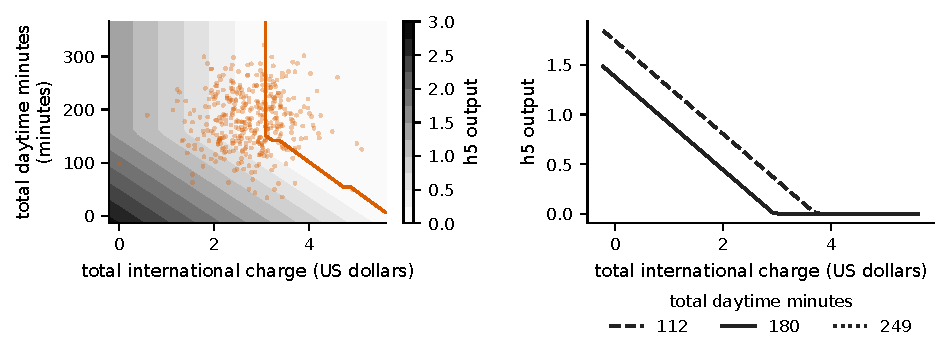
\includegraphics[width=\linewidth,height=0.88\textheight,keepaspectratio]{figures/churn100-s2-c2/ann_90-partial-1264.pdf}
\caption{Calls with low usage: This part's own output, unit h5 (the output of 'Calls with low usage'), on its own scale (its activation), with every other input at the typical case; it is active for 2771 of 4000. Left: its output over its two main inputs (orange line: where it switches on; dots: the data); right: slices at three values of the second input.}
\label{fig:churn100s2c2:plot-ann90-6}
\end{figure}
\begin{figure}[H]\centering
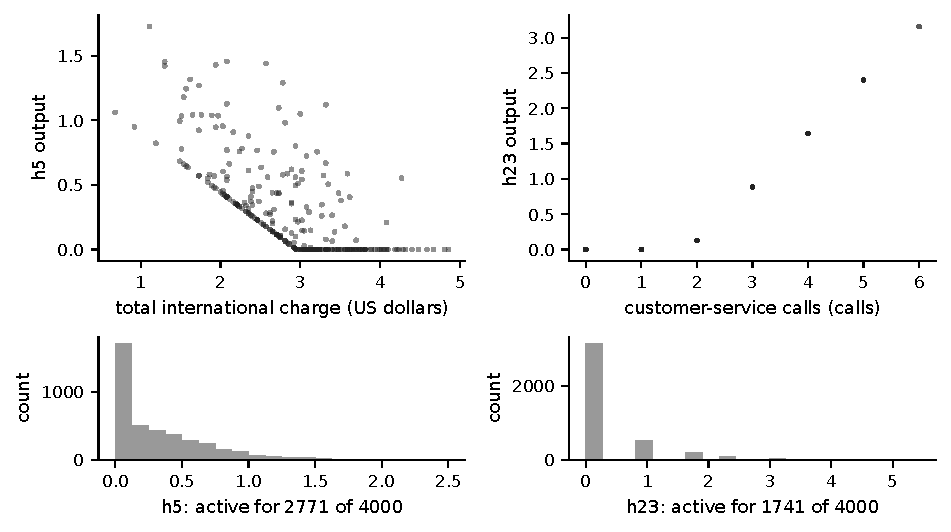
\includegraphics[width=\linewidth,height=0.88\textheight,keepaspectratio]{figures/churn100-s2-c2/ann_90-units.pdf}
\caption{Calls with low usage: This part's hidden units: each unit's output against its main numeric input (top) and how often it is active (bottom).}
\label{fig:churn100s2c2:plot-ann90-7}
\end{figure}
\par\smallskip\noindent{\small Technical detail: \ref{tech:ann90}.\par}
\subsubsection{Many service calls}\label{rd:ann91}
\noindent{\footnotesize Part of: Service calls (\ref{rd:ann96}).\par}
\noindent{\small Figure~\ref{fig:churn100s2c2:parts-ann91} shows what feeds this part; Figure~\ref{fig:churn100s2c2:units-ann91} its units and every connection into them (dashed boxes: connections from or to other parts, drawn in their own sections).\par}
\begin{figure}[H]\centering
\resizebox{!}{\ifdim\height>0.5\textheight 0.5\textheight\else\height\fi}{%
\resizebox{\ifdim\width>\linewidth\linewidth\else\width\fi}{!}{%
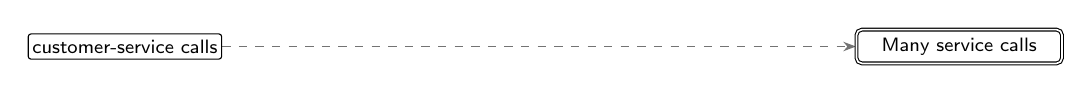
\begin{tikzpicture}[
  font=\sffamily\scriptsize, >={Stealth[length=1.6mm]},
  inp/.style={draw, rounded corners=1pt, fill=white, inner sep=1.5pt, minimum height=3.2mm, anchor=east},
  abox/.style={draw, thick, rounded corners=2pt, align=center, inner sep=3pt, minimum height=6mm, text width=42mm},
  outp/.style={draw, double, rounded corners=2pt, fill=white, align=center, inner sep=3pt, text width=24mm},
  agg/.style={draw=black!55},
]
\node[inp] (i0) at (0,-0.0) {customer-service calls};
\node[outp] (out) at (9.36,0) {Many service calls};
\begin{scope}[on background layer]
\draw[->, agg, thin, dashed] (i0.east) -- (out.west);
\end{scope}
\end{tikzpicture}}}%
\caption{Many service calls: what feeds it, one level down.}
\label{fig:churn100s2c2:parts-ann91}
\end{figure}
\begin{figure}[H]\centering
\resizebox{\ifdim\width>\linewidth\linewidth\else\width\fi}{!}{%
\definecolor{netup}{HTML}{D95F02}\definecolor{netdown}{HTML}{1B9E77}\definecolor{netmixed}{HTML}{7F7F7F}%
\begin{tikzpicture}[
  font=\sffamily\scriptsize, >={Stealth[length=1.4mm]},
  inp/.style={draw, circle, fill=white, minimum size=3.2mm, inner sep=0pt},
  hid/.style={draw, circle, fill=white, minimum size=5.2mm, inner sep=0.5pt, font=\sffamily\tiny},
  exitbox/.style={draw, thick, rectangle, fill=white, align=center, text width=17mm, minimum height=5mm, inner sep=1.5pt, font=\sffamily\tiny},
  sumbox/.style={draw, thick, dashed, rectangle, fill=white, align=center, text width=17mm, minimum height=5mm, inner sep=1.5pt, font=\sffamily\tiny},
  outp/.style={draw, thick, regular polygon, regular polygon sides=6, fill=white, minimum size=10mm, inner sep=0pt, font=\sffamily\tiny, align=center},
  stub/.style={draw, dashed, rounded corners=2pt, fill=white, align=center, inner sep=2pt, font=\sffamily\tiny, text width=15mm},
  inlab/.style={font=\sffamily\tiny, align=center, text width=15mm, inner sep=1pt, fill=white, fill opacity=0.8, text opacity=1},
  wpos/.style={draw=NavyBlue}, wneg/.style={draw=BrickRed}, wagg/.style={draw=black!45, line width=1.2pt},
  wmix/.style={draw=Plum},
]
\node[exitbox] (n7208) at (1.8,1.9) {Many service calls $\uparrow$};
\node[inp, draw=netup, very thick] (ninxxnumberxcustomerxservicexcalls) at (1.8,0.0) {};
\path (ninxxnumberxcustomerxservicexcalls.south) node[inlab, anchor=north] (labninxxnumberxcustomerxservicexcalls) {customer-service calls $\uparrow$};
\node[stub] (ntoxxServicexcalls) at (1.8,3.45) {to Service calls};
\begin{scope}[on background layer]
\node[fit=(n7208) , inner sep=8pt, rounded corners=5pt, fill=ForestGreen!10, draw=ForestGreen!45] (clu0) {};
\draw[->, wpos, line width=0.45pt] (ninxxnumberxcustomerxservicexcalls) -- (n7208);
\draw[->, wpos, line width=0.78pt] (n7208) -- (ntoxxServicexcalls);
\end{scope}
\node[font=\sffamily\scriptsize\bfseries, text=ForestGreen!55!black, anchor=south west, inner sep=1pt, fill=white, fill opacity=0.85, text opacity=1] at (clu0.north west) {Many service calls};
\end{tikzpicture}}%
\caption{Many service calls: its units and every connection into them. Blue: positive weight (raises the score); red: negative weight (lowers it); thicker: larger weight. Orange outline and up arrow: raises the final prediction; teal and down arrow: lowers it; grey and double arrow: depends.}
\label{fig:churn100s2c2:units-ann91}
\end{figure}
\paragraph{Hypothesis.} This part raises the chance of leaving from 4 customer-service calls upwards, slowly at first, then faster.\,{\scriptsize\textcolor{NavyBlue}{[C122]}}
\paragraph{Evidence.} It acts on 318 of 4000 training customers, 159 of whom left; for the typical customer it acts on, the chance is about 7\% without it and about 12\% with it.\,{\scriptsize\textcolor{NavyBlue}{[C123]}} Through it, the chance rises slowly at first, then faster: going from 0 to 4 calls moves a typical such customer's chance from about 1\% to about 2\%.\,{\scriptsize\textcolor{NavyBlue}{[C122]}} Its formula reproduces the part exactly on all 4000 training customers.\,{\scriptsize\textcolor{NavyBlue}{[C124]}}
\par\noindent{\small Evidence plots: Figure~\ref{fig:churn100s2c2:plot-ann91-0}, Figure~\ref{fig:churn100s2c2:plot-ann91-1}.\par}
\par\noindent{\small Figure~\ref{fig:churn100s2c2:plot-ann91-0} shows this part's own output, unit h11: it switches on at about 3.194 calls of customer-service calls, and is zero below.\par}
\begin{figure}[H]\centering
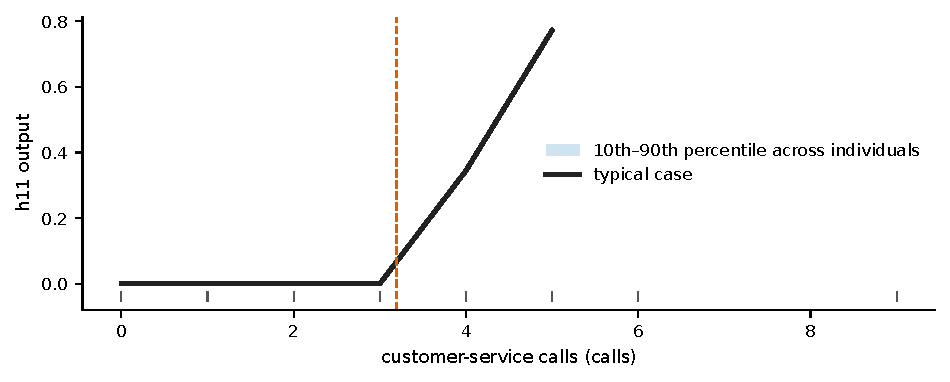
\includegraphics[width=\linewidth,height=0.88\textheight,keepaspectratio]{figures/churn100-s2-c2/ann_91-partial-7208.pdf}
\caption{Many service calls: This part's own output, unit h11 (the output of 'Many service calls'), on its own scale (its activation), with every other input at the typical case; it is active for 318 of 4000. Bold: the typical case; band: 10th to 90th percentile across individuals; dashed: where it switches on; ticks: the data.}
\label{fig:churn100s2c2:plot-ann91-0}
\end{figure}
\begin{figure}[H]\centering
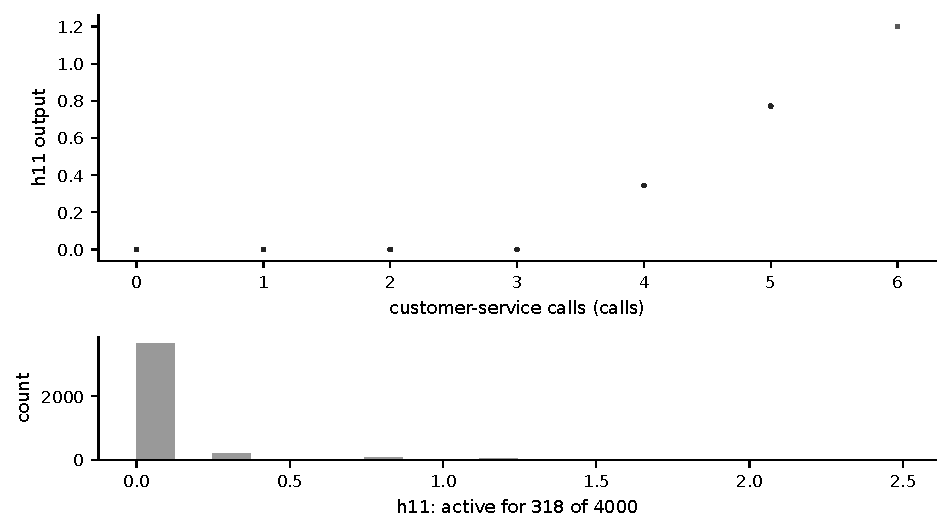
\includegraphics[width=\linewidth,height=0.88\textheight,keepaspectratio]{figures/churn100-s2-c2/ann_91-units.pdf}
\caption{Many service calls: This part's hidden units: each unit's output against its main numeric input (top) and how often it is active (bottom).}
\label{fig:churn100s2c2:plot-ann91-1}
\end{figure}
\par\smallskip\noindent{\small Technical detail: \ref{tech:ann91}.\par}
\subsubsection{Voice-mail discount}\label{rd:ann92}
\noindent{\footnotesize Part of: The whole model (\ref{rd:ann97}).\par}
\noindent{\small Figure~\ref{fig:churn100s2c2:parts-ann92} shows what feeds this part; Figure~\ref{fig:churn100s2c2:units-ann92} its units and every connection into them (dashed boxes: connections from or to other parts, drawn in their own sections).\par}
\begin{figure}[H]\centering
\resizebox{!}{\ifdim\height>0.5\textheight 0.5\textheight\else\height\fi}{%
\resizebox{\ifdim\width>\linewidth\linewidth\else\width\fi}{!}{%
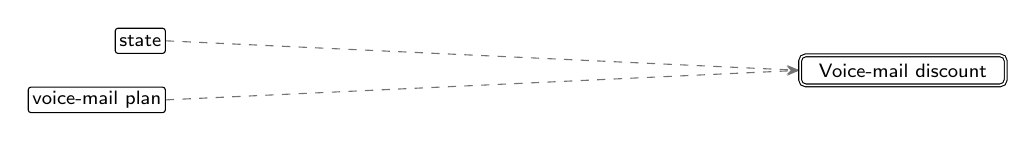
\begin{tikzpicture}[
  font=\sffamily\scriptsize, >={Stealth[length=1.6mm]},
  inp/.style={draw, rounded corners=1pt, fill=white, inner sep=1.5pt, minimum height=3.2mm, anchor=east},
  abox/.style={draw, thick, rounded corners=2pt, align=center, inner sep=3pt, minimum height=6mm, text width=42mm},
  outp/.style={draw, double, rounded corners=2pt, fill=white, align=center, inner sep=3pt, text width=24mm},
  agg/.style={draw=black!55},
]
\node[inp] (i0) at (0,0.375) {state};
\node[inp] (i1) at (0,-0.375) {voice-mail plan};
\node[outp] (out) at (9.36,0) {Voice-mail discount};
\begin{scope}[on background layer]
\draw[->, agg, thin, dashed] (i0.east) -- (out.west);
\draw[->, agg, thin, dashed] (i1.east) -- (out.west);
\end{scope}
\end{tikzpicture}}}%
\caption{Voice-mail discount: what feeds it, one level down.}
\label{fig:churn100s2c2:parts-ann92}
\end{figure}
\begin{figure}[H]\centering
\resizebox{\ifdim\width>\linewidth\linewidth\else\width\fi}{!}{%
\definecolor{netup}{HTML}{D95F02}\definecolor{netdown}{HTML}{1B9E77}\definecolor{netmixed}{HTML}{7F7F7F}%
\begin{tikzpicture}[
  font=\sffamily\scriptsize, >={Stealth[length=1.4mm]},
  inp/.style={draw, circle, fill=white, minimum size=3.2mm, inner sep=0pt},
  hid/.style={draw, circle, fill=white, minimum size=5.2mm, inner sep=0.5pt, font=\sffamily\tiny},
  exitbox/.style={draw, thick, rectangle, fill=white, align=center, text width=17mm, minimum height=5mm, inner sep=1.5pt, font=\sffamily\tiny},
  sumbox/.style={draw, thick, dashed, rectangle, fill=white, align=center, text width=17mm, minimum height=5mm, inner sep=1.5pt, font=\sffamily\tiny},
  outp/.style={draw, thick, regular polygon, regular polygon sides=6, fill=white, minimum size=10mm, inner sep=0pt, font=\sffamily\tiny, align=center},
  stub/.style={draw, dashed, rounded corners=2pt, fill=white, align=center, inner sep=2pt, font=\sffamily\tiny, text width=15mm},
  inlab/.style={font=\sffamily\tiny, align=center, text width=15mm, inner sep=1pt, fill=white, fill opacity=0.8, text opacity=1},
  wpos/.style={draw=NavyBlue}, wneg/.style={draw=BrickRed}, wagg/.style={draw=black!45, line width=1.2pt},
  wmix/.style={draw=Plum},
]
\node[hid] (n14955) at (1.9,1.9) {h22};
\node[hid] (n4051) at (1.9,4.6) {h8};
\node[hid] (n13852) at (0.4,1.9) {h20};
\node[hid] (n1133) at (1.9,3.25) {h4};
\node[hid] (n5577) at (3.4,1.9) {h10};
\node[inp, draw=netmixed, very thick] (ngrpxxstate) at (1.0,0.0) {};
\path (ngrpxxstate.south) node[inlab, anchor=north] (labngrpxxstate) {state (26 of 51 used) $\updownarrow$};
\node[inp, draw=netdown, very thick] (ninxxvoicexmailxplan) at (2.8,0.0) {};
\path (ninxxvoicexmailxplan.south) node[inlab, anchor=north] (labninxxvoicexmailxplan) {a voice-mail plan $\downarrow$};
\node[stub] (ntoxxthexmodelxoutput) at (1.9,6.15) {to the model output};
\begin{scope}[on background layer]
\node[fit=(n14955) (n4051) (n13852) (n1133) (n5577) , inner sep=8pt, rounded corners=5pt, fill=Orchid!10, draw=Orchid!45] (clu0) {};
\draw[->, wpos, line width=0.58pt] (n1133) -- (n4051);
\draw[->, wpos, line width=0.32pt] (n5577) -- (n1133);
\draw[->, wpos, line width=0.33pt] (n13852) -- (n1133);
\draw[->, wpos, line width=0.26pt] (n14955) -- (n1133);
\draw[->, wpos, line width=0.29pt] (ninxxvoicexmailxplan) -- (n1133);
\draw[->, wpos, line width=0.59pt] (ninxxvoicexmailxplan) -- (n5577);
\draw[->, wpos, line width=0.60pt] (ninxxvoicexmailxplan) -- (n13852);
\draw[->, wneg, line width=0.56pt] (n1133) -- (ntoxxthexmodelxoutput);
\draw[->, wneg, line width=0.60pt] (n4051) -- (ntoxxthexmodelxoutput);
\draw[->, wpos, line width=0.60pt] (ngrpxxstate) -- node[pos=0.8, sloped, above, font=\sffamily\tiny, inner sep=1pt, fill=white, fill opacity=0.8, text opacity=1] {+0.99} (n14955);
\end{scope}
\node[font=\sffamily\scriptsize\bfseries, text=Orchid!55!black, anchor=south west, inner sep=1pt, fill=white, fill opacity=0.85, text opacity=1] at (clu0.north west) {Voice-mail discount};
\end{tikzpicture}}%
\caption{Voice-mail discount: its units and every connection into them. Blue: positive weight (raises the score); red: negative weight (lowers it); thicker: larger weight. Orange outline and up arrow: raises the final prediction; teal and down arrow: lowers it; grey and double arrow: depends.}
\label{fig:churn100s2c2:units-ann92}
\end{figure}
\paragraph{Hypothesis.} This part gives customers with a voice-mail plan a further discount on the chance of leaving.\,{\scriptsize\textcolor{NavyBlue}{[C119]}}
\paragraph{Evidence.} Through it, a voice-mail plan lowers a typical customer's chance from about 1\% to under 1\%, and customers in North Carolina get under 1\% instead of about 1\%.\,{\scriptsize\textcolor{NavyBlue}{[C119, C120]}} Its formula reproduces the part exactly on all 4000 training customers.\,{\scriptsize\textcolor{NavyBlue}{[C121]}}
\par\noindent{\small Evidence plots: Figure~\ref{fig:churn100s2c2:plot-ann92-0}, Figure~\ref{fig:churn100s2c2:plot-ann92-1}.\par}
\begin{figure}[H]\centering
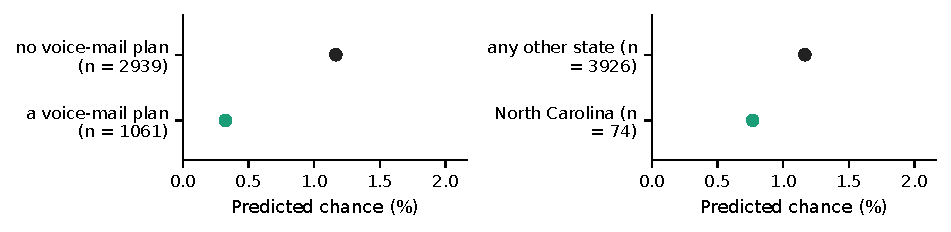
\includegraphics[width=\linewidth,height=0.88\textheight,keepaspectratio]{figures/churn100-s2-c2/ann_92-categories-small.pdf}
\caption{Voice-mail discount: The predicted value for the typical case at each level, through this part (n = training customers; grey: fewer than 20).}
\label{fig:churn100s2c2:plot-ann92-0}
\end{figure}
\begin{figure}[H]\centering
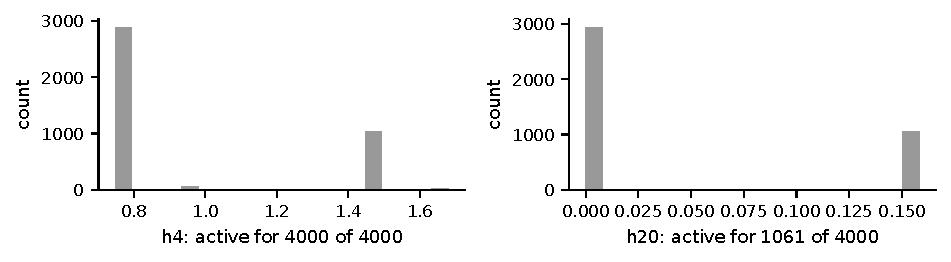
\includegraphics[width=\linewidth,height=0.88\textheight,keepaspectratio]{figures/churn100-s2-c2/ann_92-units.pdf}
\caption{Voice-mail discount: This part's hidden units: each unit's output against its main numeric input (top) and how often it is active (bottom).}
\label{fig:churn100s2c2:plot-ann92-1}
\end{figure}
\par\smallskip\noindent{\small Technical detail: \ref{tech:ann92}.\par}
\subsubsection{State units}\label{rd:ann95}
\noindent{\footnotesize Part of: The whole model (\ref{rd:ann97}).\par}
\noindent{\small Figure~\ref{fig:churn100s2c2:parts-ann95} shows what feeds this part; Figure~\ref{fig:churn100s2c2:units-ann95} its units and every connection into them (dashed boxes: connections from or to other parts, drawn in their own sections).\par}
\begin{figure}[H]\centering
\resizebox{!}{\ifdim\height>0.5\textheight 0.5\textheight\else\height\fi}{%
\resizebox{\ifdim\width>\linewidth\linewidth\else\width\fi}{!}{%
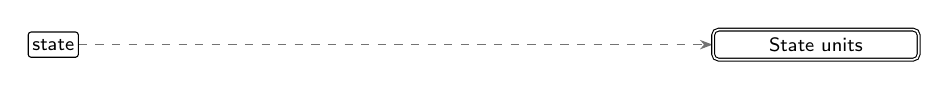
\begin{tikzpicture}[
  font=\sffamily\scriptsize, >={Stealth[length=1.6mm]},
  inp/.style={draw, rounded corners=1pt, fill=white, inner sep=1.5pt, minimum height=3.2mm, anchor=east},
  abox/.style={draw, thick, rounded corners=2pt, align=center, inner sep=3pt, minimum height=6mm, text width=42mm},
  outp/.style={draw, double, rounded corners=2pt, fill=white, align=center, inner sep=3pt, text width=24mm},
  agg/.style={draw=black!55},
]
\node[inp] (i0) at (0,-0.0) {state};
\node[outp] (out) at (9.36,0) {State units};
\begin{scope}[on background layer]
\draw[->, agg, thin, dashed] (i0.east) -- (out.west);
\end{scope}
\end{tikzpicture}}}%
\caption{State units: what feeds it, one level down.}
\label{fig:churn100s2c2:parts-ann95}
\end{figure}
\begin{figure}[H]\centering
\resizebox{\ifdim\width>\linewidth\linewidth\else\width\fi}{!}{%
\definecolor{netup}{HTML}{D95F02}\definecolor{netdown}{HTML}{1B9E77}\definecolor{netmixed}{HTML}{7F7F7F}%
\begin{tikzpicture}[
  font=\sffamily\scriptsize, >={Stealth[length=1.4mm]},
  inp/.style={draw, circle, fill=white, minimum size=3.2mm, inner sep=0pt},
  hid/.style={draw, circle, fill=white, minimum size=5.2mm, inner sep=0.5pt, font=\sffamily\tiny},
  exitbox/.style={draw, thick, rectangle, fill=white, align=center, text width=17mm, minimum height=5mm, inner sep=1.5pt, font=\sffamily\tiny},
  sumbox/.style={draw, thick, dashed, rectangle, fill=white, align=center, text width=17mm, minimum height=5mm, inner sep=1.5pt, font=\sffamily\tiny},
  outp/.style={draw, thick, regular polygon, regular polygon sides=6, fill=white, minimum size=10mm, inner sep=0pt, font=\sffamily\tiny, align=center},
  stub/.style={draw, dashed, rounded corners=2pt, fill=white, align=center, inner sep=2pt, font=\sffamily\tiny, text width=15mm},
  inlab/.style={font=\sffamily\tiny, align=center, text width=15mm, inner sep=1pt, fill=white, fill opacity=0.8, text opacity=1},
  wpos/.style={draw=NavyBlue}, wneg/.style={draw=BrickRed}, wagg/.style={draw=black!45, line width=1.2pt},
  wmix/.style={draw=Plum},
]
\node[hid] (n8418) at (9.35,1.9) {h13};
\node[hid] (n16902) at (4.85,3.25) {h25};
\node[hid] (n7647) at (6.35,3.25) {h12};
\node[hid] (n16344) at (6.35,1.9) {h24};
\node[hid] (n4967) at (7.85,1.9) {h9};
\node[hid] (n11261) at (1.85,1.9) {h17};
\node[hid] (n13725) at (4.85,1.9) {h19};
\node[hid] (n8896) at (10.85,1.9) {h14};
\node[hid] (n10332) at (0.35,1.9) {h16};
\node[hid] (n13551) at (3.35,1.9) {h18};
\node[inp, draw=netmixed, very thick] (ngrpxxstate) at (5.6,0.0) {};
\path (ngrpxxstate.south) node[inlab, anchor=north] (labngrpxxstate) {state (26 of 51 used) $\updownarrow$};
\node[stub] (ntoxxthexmodelxoutput) at (5.6,4.8) {to the model output};
\begin{scope}[on background layer]
\node[fit=(n8418) (n16902) (n7647) (n16344) (n4967) (n11261) (n13725) (n8896) (n10332) (n13551) , inner sep=8pt, rounded corners=5pt, fill=Goldenrod!10, draw=Goldenrod!45] (clu0) {};
\draw[->, wpos, line width=0.59pt] (n4967) -- (n7647);
\draw[->, wpos, line width=0.60pt] (n11261) -- (n16902);
\draw[->, wneg, line width=0.25pt] (n7647) -- (ntoxxthexmodelxoutput);
\draw[->, wneg, line width=0.25pt] (n8418) -- (ntoxxthexmodelxoutput);
\draw[->, wneg, line width=0.25pt] (n8896) -- (ntoxxthexmodelxoutput);
\draw[->, wpos, line width=0.29pt] (n10332) -- (ntoxxthexmodelxoutput);
\draw[->, wpos, line width=0.27pt] (n13551) -- (ntoxxthexmodelxoutput);
\draw[->, wpos, line width=0.27pt] (n13725) -- (ntoxxthexmodelxoutput);
\draw[->, wpos, line width=0.27pt] (n16344) -- (ntoxxthexmodelxoutput);
\draw[->, wpos, line width=0.27pt] (n16902) -- (ntoxxthexmodelxoutput);
\draw[->, wpos, line width=0.59pt] (ngrpxxstate) -- node[pos=0.8, sloped, above, font=\sffamily\tiny, inner sep=1pt, fill=white, fill opacity=0.8, text opacity=1] {+0.98} (n4967);
\draw[->, wmix, line width=0.60pt] (ngrpxxstate) -- node[pos=0.8, sloped, above, font=\sffamily\tiny, inner sep=1pt, fill=white, fill opacity=0.8, text opacity=1] {2 edges, -0.02 to +0.99} (n11261);
\draw[->, wpos, line width=0.60pt] (ngrpxxstate) -- node[pos=0.8, sloped, above, font=\sffamily\tiny, inner sep=1pt, fill=white, fill opacity=0.8, text opacity=1] {+1.00} (n13551);
\draw[->, wpos, line width=0.56pt] (ngrpxxstate) -- node[pos=0.8, sloped, above, font=\sffamily\tiny, inner sep=1pt, fill=white, fill opacity=0.8, text opacity=1] {+0.89} (n10332);
\draw[->, wpos, line width=0.60pt] (ngrpxxstate) -- node[pos=0.8, sloped, above, font=\sffamily\tiny, inner sep=1pt, fill=white, fill opacity=0.8, text opacity=1] {+1.01} (n8896);
\draw[->, wpos, line width=0.60pt] (ngrpxxstate) -- node[pos=0.8, sloped, above, font=\sffamily\tiny, inner sep=1pt, fill=white, fill opacity=0.8, text opacity=1] {+0.99} (n8418);
\draw[->, wpos, line width=0.60pt] (ngrpxxstate) -- node[pos=0.8, sloped, above, font=\sffamily\tiny, inner sep=1pt, fill=white, fill opacity=0.8, text opacity=1] {+0.99} (n13725);
\draw[->, wpos, line width=0.60pt] (ngrpxxstate) -- node[pos=0.8, sloped, above, font=\sffamily\tiny, inner sep=1pt, fill=white, fill opacity=0.8, text opacity=1] {+1.00} (n16344);
\end{scope}
\node[font=\sffamily\scriptsize\bfseries, text=Goldenrod!55!black, anchor=south west, inner sep=1pt, fill=white, fill opacity=0.85, text opacity=1] at (clu0.north west) {State units};
\end{tikzpicture}}%
\caption{State units: its units and every connection into them. Blue: positive weight (raises the score); red: negative weight (lowers it); thicker: larger weight. Orange outline and up arrow: raises the final prediction; teal and down arrow: lowers it; grey and double arrow: depends.}
\label{fig:churn100s2c2:units-ann95}
\end{figure}
\paragraph{Hypothesis.} This part reads only the state and raises the chance of leaving in a few states, most in Washington and Montana.\,{\scriptsize\textcolor{NavyBlue}{[C125, C126]}}
\paragraph{Evidence.} Through it, a typical customer's chance goes from about 1\% to about 2\% in Washington and in Montana, and up by less than a point in Kentucky and Ohio.\,{\scriptsize\textcolor{NavyBlue}{[C125, C126, C127, C128]}} In Arizona, Delaware, North Dakota and Nevada it lowers the chance by less than a tenth of a point.\,{\scriptsize\textcolor{NavyBlue}{[C129, C130, C131, C132]}} Its formula reproduces the part exactly on all 4000 training customers.\,{\scriptsize\textcolor{NavyBlue}{[C133]}}
\par\noindent{\small Evidence plots: Figure~\ref{fig:churn100s2c2:plot-ann95-0}, Figure~\ref{fig:churn100s2c2:plot-ann95-1}.\par}
\begin{figure}[H]\centering
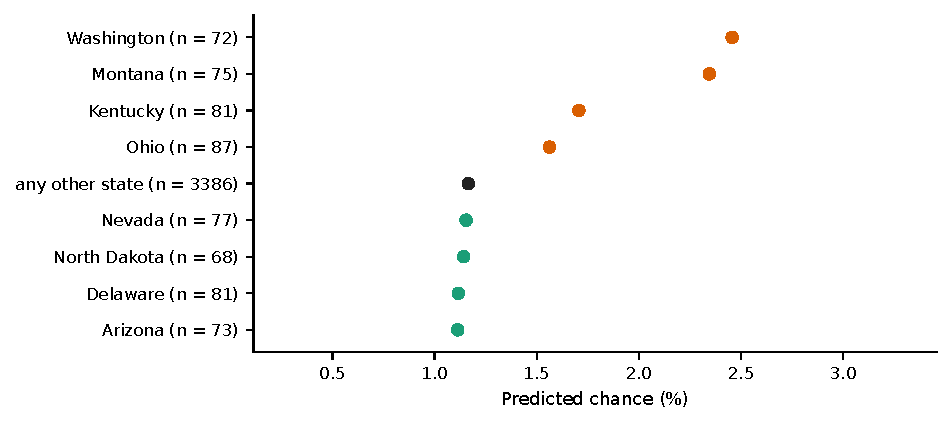
\includegraphics[width=\linewidth,height=0.88\textheight,keepaspectratio]{figures/churn100-s2-c2/ann_95-categories-C125.pdf}
\caption{State units: The predicted value for the typical case at each level, through this part (n = training customers; grey: fewer than 20).}
\label{fig:churn100s2c2:plot-ann95-0}
\end{figure}
\begin{figure}[H]\centering
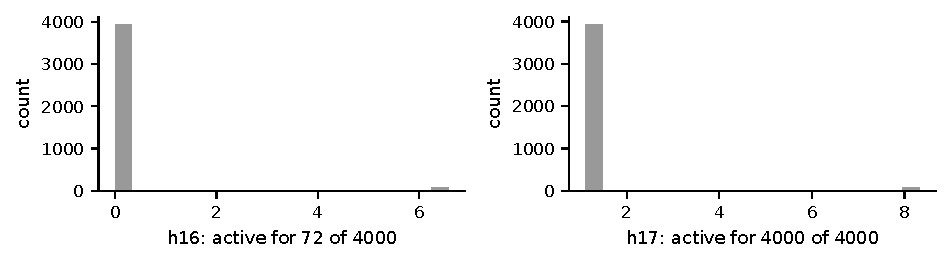
\includegraphics[width=\linewidth,height=0.88\textheight,keepaspectratio]{figures/churn100-s2-c2/ann_95-units.pdf}
\caption{State units: This part's hidden units: each unit's output against its main numeric input (top) and how often it is active (bottom).}
\label{fig:churn100s2c2:plot-ann95-1}
\end{figure}
\par\smallskip\noindent{\small Technical detail: \ref{tech:ann95}.\par}
\subsubsection{Area-code unit}\label{rd:ann94}
\noindent{\footnotesize Part of: The whole model (\ref{rd:ann97}).\par}
\noindent{\small Figure~\ref{fig:churn100s2c2:parts-ann94} shows what feeds this part; Figure~\ref{fig:churn100s2c2:units-ann94} its units and every connection into them (dashed boxes: connections from or to other parts, drawn in their own sections).\par}
\begin{figure}[H]\centering
\resizebox{!}{\ifdim\height>0.5\textheight 0.5\textheight\else\height\fi}{%
\resizebox{\ifdim\width>\linewidth\linewidth\else\width\fi}{!}{%
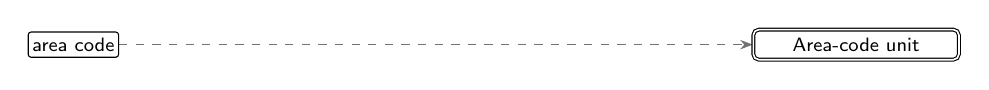
\begin{tikzpicture}[
  font=\sffamily\scriptsize, >={Stealth[length=1.6mm]},
  inp/.style={draw, rounded corners=1pt, fill=white, inner sep=1.5pt, minimum height=3.2mm, anchor=east},
  abox/.style={draw, thick, rounded corners=2pt, align=center, inner sep=3pt, minimum height=6mm, text width=42mm},
  outp/.style={draw, double, rounded corners=2pt, fill=white, align=center, inner sep=3pt, text width=24mm},
  agg/.style={draw=black!55},
]
\node[inp] (i0) at (0,-0.0) {area code};
\node[outp] (out) at (9.36,0) {Area-code unit};
\begin{scope}[on background layer]
\draw[->, agg, thin, dashed] (i0.east) -- (out.west);
\end{scope}
\end{tikzpicture}}}%
\caption{Area-code unit: what feeds it, one level down.}
\label{fig:churn100s2c2:parts-ann94}
\end{figure}
\begin{figure}[H]\centering
\resizebox{\ifdim\width>\linewidth\linewidth\else\width\fi}{!}{%
\definecolor{netup}{HTML}{D95F02}\definecolor{netdown}{HTML}{1B9E77}\definecolor{netmixed}{HTML}{7F7F7F}%
\begin{tikzpicture}[
  font=\sffamily\scriptsize, >={Stealth[length=1.4mm]},
  inp/.style={draw, circle, fill=white, minimum size=3.2mm, inner sep=0pt},
  hid/.style={draw, circle, fill=white, minimum size=5.2mm, inner sep=0.5pt, font=\sffamily\tiny},
  exitbox/.style={draw, thick, rectangle, fill=white, align=center, text width=17mm, minimum height=5mm, inner sep=1.5pt, font=\sffamily\tiny},
  sumbox/.style={draw, thick, dashed, rectangle, fill=white, align=center, text width=17mm, minimum height=5mm, inner sep=1.5pt, font=\sffamily\tiny},
  outp/.style={draw, thick, regular polygon, regular polygon sides=6, fill=white, minimum size=10mm, inner sep=0pt, font=\sffamily\tiny, align=center},
  stub/.style={draw, dashed, rounded corners=2pt, fill=white, align=center, inner sep=2pt, font=\sffamily\tiny, text width=15mm},
  inlab/.style={font=\sffamily\tiny, align=center, text width=15mm, inner sep=1pt, fill=white, fill opacity=0.8, text opacity=1},
  wpos/.style={draw=NavyBlue}, wneg/.style={draw=BrickRed}, wagg/.style={draw=black!45, line width=1.2pt},
  wmix/.style={draw=Plum},
]
\node[hid] (n14653) at (1.05,1.9) {h21};
\node[hid] (n161) at (2.55,1.9) {h1};
\node[inp, draw=netup, very thick] (ninxxareaxcodex415) at (2.7,0.0) {};
\path (ninxxareaxcodex415.south) node[inlab, anchor=north] (labninxxareaxcodex415) {area code 415 $\uparrow$};
\node[inp, draw=netdown, very thick] (ninxxareaxcodex408) at (0.9,0.0) {};
\path (ninxxareaxcodex408.south) node[inlab, anchor=north] (labninxxareaxcodex408) {area code 408 $\downarrow$};
\node[stub] (ntoxxthexmodelxoutput) at (1.8,3.45) {to the model output};
\begin{scope}[on background layer]
\node[fit=(n14653) (n161) , inner sep=8pt, rounded corners=5pt, fill=Cerulean!10, draw=Cerulean!45] (clu0) {};
\draw[->, wpos, line width=0.45pt] (ninxxareaxcodex415) -- (n161);
\draw[->, wneg, line width=0.44pt] (ninxxareaxcodex408) -- (n14653);
\draw[->, wpos, line width=0.27pt] (n161) -- (ntoxxthexmodelxoutput);
\draw[->, wneg, line width=0.34pt] (n14653) -- (ntoxxthexmodelxoutput);
\end{scope}
\node[font=\sffamily\scriptsize\bfseries, text=Cerulean!55!black, anchor=south west, inner sep=1pt, fill=white, fill opacity=0.85, text opacity=1] at (clu0.north west) {Area-code unit};
\end{tikzpicture}}%
\caption{Area-code unit: its units and every connection into them. Blue: positive weight (raises the score); red: negative weight (lowers it); thicker: larger weight. Orange outline and up arrow: raises the final prediction; teal and down arrow: lowers it; grey and double arrow: depends.}
\label{fig:churn100s2c2:units-ann94}
\end{figure}
\paragraph{Hypothesis.} This part reads the area code and barely changes the predictions.\,{\scriptsize\textcolor{NavyBlue}{[C137]}}
\paragraph{Evidence.} Through it, a typical customer's chance stays at about 1\% in area codes 408 and 510, as in area code 415.\,{\scriptsize\textcolor{NavyBlue}{[C134, C135]}} Switching it off changes the predictions by at most half a point.\,{\scriptsize\textcolor{NavyBlue}{[C137]}} Its formula reproduces the part exactly on all 4000 training customers.\,{\scriptsize\textcolor{NavyBlue}{[C138]}}
\par\noindent{\small Evidence plots: Figure~\ref{fig:churn100s2c2:plot-ann94-0}, Figure~\ref{fig:churn100s2c2:plot-ann94-1}.\par}
\begin{figure}[H]\centering
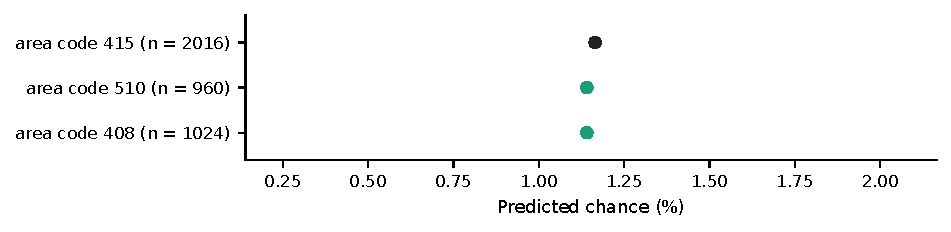
\includegraphics[width=\linewidth,height=0.88\textheight,keepaspectratio]{figures/churn100-s2-c2/ann_94-categories-small.pdf}
\caption{Area-code unit: The predicted value for the typical case at each level, through this part (n = training customers; grey: fewer than 20).}
\label{fig:churn100s2c2:plot-ann94-0}
\end{figure}
\begin{figure}[H]\centering
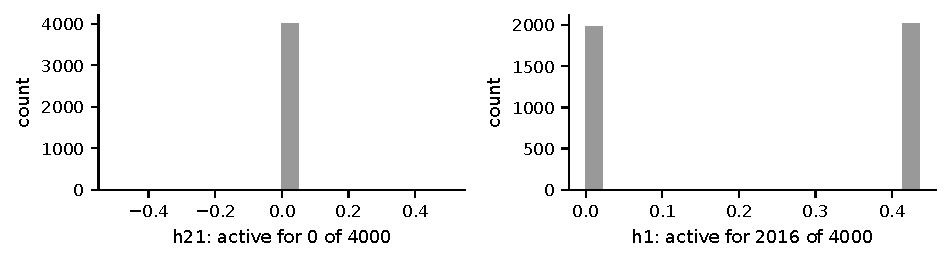
\includegraphics[width=\linewidth,height=0.88\textheight,keepaspectratio]{figures/churn100-s2-c2/ann_94-units.pdf}
\caption{Area-code unit: This part's hidden units: each unit's output against its main numeric input (top) and how often it is active (bottom).}
\label{fig:churn100s2c2:plot-ann94-1}
\end{figure}
\par\smallskip\noindent{\small Technical detail: \ref{tech:ann94}.\par}
\subsubsection{Small Utah unit}\label{rd:ann93}
\noindent{\footnotesize Part of: The whole model (\ref{rd:ann97}).\par}
\noindent{\small Figure~\ref{fig:churn100s2c2:parts-ann93} shows what feeds this part; Figure~\ref{fig:churn100s2c2:units-ann93} its units and every connection into them (dashed boxes: connections from or to other parts, drawn in their own sections).\par}
\begin{figure}[H]\centering
\resizebox{!}{\ifdim\height>0.5\textheight 0.5\textheight\else\height\fi}{%
\resizebox{\ifdim\width>\linewidth\linewidth\else\width\fi}{!}{%
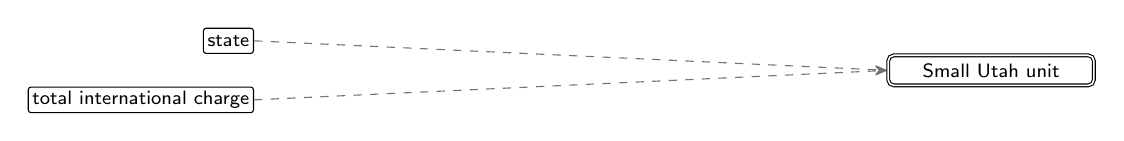
\begin{tikzpicture}[
  font=\sffamily\scriptsize, >={Stealth[length=1.6mm]},
  inp/.style={draw, rounded corners=1pt, fill=white, inner sep=1.5pt, minimum height=3.2mm, anchor=east},
  abox/.style={draw, thick, rounded corners=2pt, align=center, inner sep=3pt, minimum height=6mm, text width=42mm},
  outp/.style={draw, double, rounded corners=2pt, fill=white, align=center, inner sep=3pt, text width=24mm},
  agg/.style={draw=black!55},
]
\node[inp] (i0) at (0,0.375) {state};
\node[inp] (i1) at (0,-0.375) {total international charge};
\node[outp] (out) at (9.36,0) {Small Utah unit};
\begin{scope}[on background layer]
\draw[->, agg, thin, dashed] (i0.east) -- (out.west);
\draw[->, agg, thin, dashed] (i1.east) -- (out.west);
\end{scope}
\end{tikzpicture}}}%
\caption{Small Utah unit: what feeds it, one level down.}
\label{fig:churn100s2c2:parts-ann93}
\end{figure}
\begin{figure}[H]\centering
\resizebox{\ifdim\width>\linewidth\linewidth\else\width\fi}{!}{%
\definecolor{netup}{HTML}{D95F02}\definecolor{netdown}{HTML}{1B9E77}\definecolor{netmixed}{HTML}{7F7F7F}%
\begin{tikzpicture}[
  font=\sffamily\scriptsize, >={Stealth[length=1.4mm]},
  inp/.style={draw, circle, fill=white, minimum size=3.2mm, inner sep=0pt},
  hid/.style={draw, circle, fill=white, minimum size=5.2mm, inner sep=0.5pt, font=\sffamily\tiny},
  exitbox/.style={draw, thick, rectangle, fill=white, align=center, text width=17mm, minimum height=5mm, inner sep=1.5pt, font=\sffamily\tiny},
  sumbox/.style={draw, thick, dashed, rectangle, fill=white, align=center, text width=17mm, minimum height=5mm, inner sep=1.5pt, font=\sffamily\tiny},
  outp/.style={draw, thick, regular polygon, regular polygon sides=6, fill=white, minimum size=10mm, inner sep=0pt, font=\sffamily\tiny, align=center},
  stub/.style={draw, dashed, rounded corners=2pt, fill=white, align=center, inner sep=2pt, font=\sffamily\tiny, text width=15mm},
  inlab/.style={font=\sffamily\tiny, align=center, text width=15mm, inner sep=1pt, fill=white, fill opacity=0.8, text opacity=1},
  wpos/.style={draw=NavyBlue}, wneg/.style={draw=BrickRed}, wagg/.style={draw=black!45, line width=1.2pt},
  wmix/.style={draw=Plum},
]
\node[exitbox] (n252) at (1.8,1.9) {Small Utah unit $\uparrow$};
\node[inp, draw=netmixed, very thick] (ngrpxxstate) at (0.9,0.0) {};
\path (ngrpxxstate.south) node[inlab, anchor=north] (labngrpxxstate) {state (26 of 51 used) $\updownarrow$};
\node[inp, draw=netdown, very thick] (ninxxtotalxintlxcharge) at (2.7,0.0) {};
\path (ninxxtotalxintlxcharge.south) node[inlab, anchor=north] (labninxxtotalxintlxcharge) {total international charge $\downarrow$};
\node[stub] (ntoxxthexmodelxoutput) at (1.8,3.45) {to the model output};
\begin{scope}[on background layer]
\node[fit=(n252) , inner sep=8pt, rounded corners=5pt, fill=Mahogany!10, draw=Mahogany!45] (clu0) {};
\draw[->, wneg, line width=0.55pt] (ninxxtotalxintlxcharge) -- (n252);
\draw[->, wpos, line width=0.25pt] (n252) -- (ntoxxthexmodelxoutput);
\draw[->, wpos, line width=0.40pt] (ngrpxxstate) -- node[pos=0.8, sloped, above, font=\sffamily\tiny, inner sep=1pt, fill=white, fill opacity=0.8, text opacity=1] {+0.43} (n252);
\end{scope}
\node[font=\sffamily\scriptsize\bfseries, text=Mahogany!55!black, anchor=south west, inner sep=1pt, fill=white, fill opacity=0.85, text opacity=1] at (clu0.north west) {Small Utah unit};
\end{tikzpicture}}%
\caption{Small Utah unit: its units and every connection into them. Blue: positive weight (raises the score); red: negative weight (lowers it); thicker: larger weight. Orange outline and up arrow: raises the final prediction; teal and down arrow: lowers it; grey and double arrow: depends.}
\label{fig:churn100s2c2:units-ann93}
\end{figure}
\paragraph{Hypothesis.} This small part reads the international charge and being in Utah, and barely changes the predictions.\,{\scriptsize\textcolor{NavyBlue}{[C144]}}
\paragraph{Evidence.} Through it, the international charge barely changes the chance, which stays at about 1\% for the typical customer it acts on.\,{\scriptsize\textcolor{NavyBlue}{[C139]}} Switching it off changes the predictions by at most 0.2 points.\,{\scriptsize\textcolor{NavyBlue}{[C144]}} Its formula reproduces the part exactly on all 4000 training customers.\,{\scriptsize\textcolor{NavyBlue}{[C145]}}
\par\noindent{\small Evidence plots: Figure~\ref{fig:churn100s2c2:plot-ann93-0}, Figure~\ref{fig:churn100s2c2:plot-ann93-1}, Figure~\ref{fig:churn100s2c2:plot-ann93-2}, Figure~\ref{fig:churn100s2c2:plot-ann93-3}.\par}
\par\noindent{\small Figure~\ref{fig:churn100s2c2:plot-ann93-2} shows this part's own output, unit h2.\par}
\begin{figure}[H]\centering
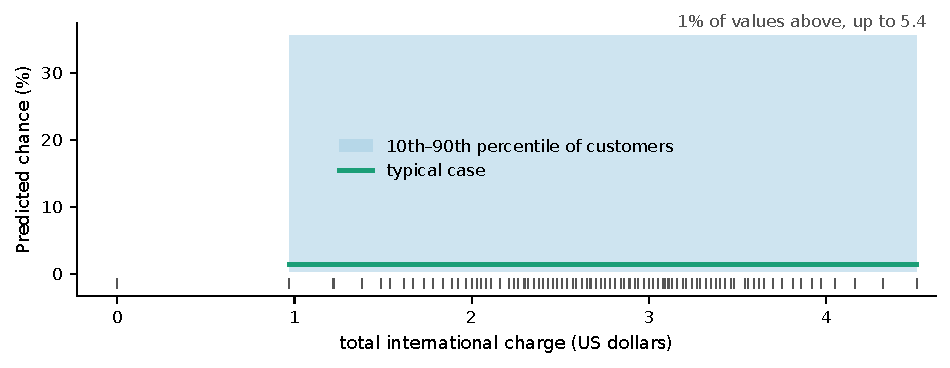
\includegraphics[width=\linewidth,height=0.88\textheight,keepaspectratio]{figures/churn100-s2-c2/ann_93-response.pdf}
\caption{Small Utah unit: Response curves through this part: the typical case (bold), the 10th to 90th percentile of individual customers (band), the fold or step point (dashed) with its spread across them (grey), and the observed values (ticks).}
\label{fig:churn100s2c2:plot-ann93-0}
\end{figure}
\begin{figure}[H]\centering
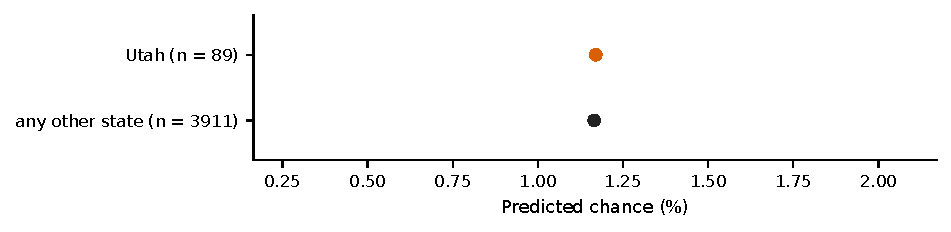
\includegraphics[width=\linewidth,height=0.88\textheight,keepaspectratio]{figures/churn100-s2-c2/ann_93-categories-small.pdf}
\caption{Small Utah unit: The predicted value for the typical case at each level, through this part (n = training customers; grey: fewer than 20).}
\label{fig:churn100s2c2:plot-ann93-1}
\end{figure}
\begin{figure}[H]\centering
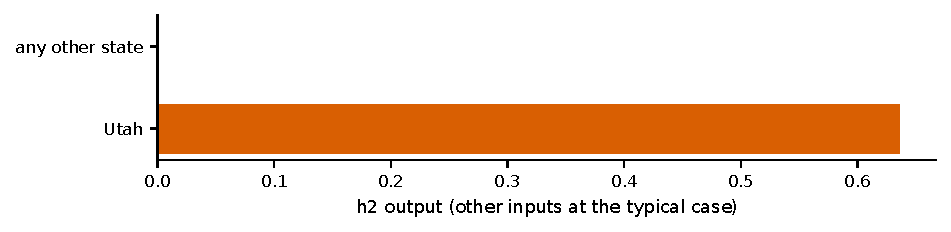
\includegraphics[width=\linewidth,height=0.88\textheight,keepaspectratio]{figures/churn100-s2-c2/ann_93-partial-252.pdf}
\caption{Small Utah unit: This part's own output, unit h2 (the output of 'Small Utah unit'), on its own scale (its activation), with every other input at the typical case; it is active for 100 of 4000. Its output for each combination of the levels it reads.}
\label{fig:churn100s2c2:plot-ann93-2}
\end{figure}
\begin{figure}[H]\centering
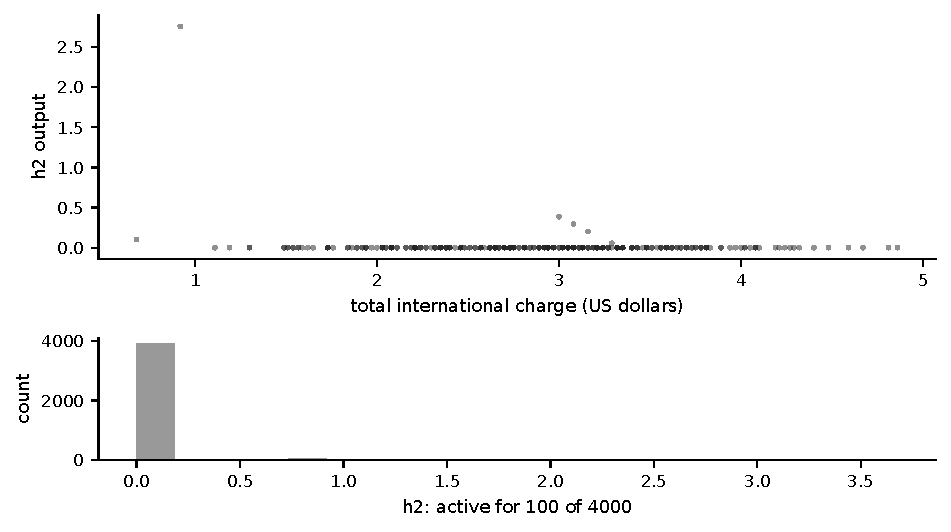
\includegraphics[width=\linewidth,height=0.88\textheight,keepaspectratio]{figures/churn100-s2-c2/ann_93-units.pdf}
\caption{Small Utah unit: This part's hidden units: each unit's output against its main numeric input (top) and how often it is active (bottom).}
\label{fig:churn100s2c2:plot-ann93-3}
\end{figure}
\par\smallskip\noindent{\small Technical detail: \ref{tech:ann93}.\par}
\subsection{Not supported by the model}
\begin{itemize}\setlength\itemsep{0pt}\small
\item C002: direction claim about total daytime minutes in the whole model: not supported by the model (14\% of patients have the opposite sign (allowed: 10\%)).
\item C017: direction claim about total evening charge in the whole model: not supported by the model (52\% of patients have the opposite sign (allowed: 10\%)).
\item C026: direction claim about state in the whole model: not supported by the model (53\% of patients have the opposite sign (allowed: 10\%)).
\item C136: subgroup claim about area code in part ann\_\allowbreak{}94: not supported by the model (its effect is negligible).
\item C141: interaction claim about total international charge and state in part ann\_\allowbreak{}93: not supported by the model (the group difference is below 0.1 log-odds; the part's own counterfactual difference has the opposite sign).
\item C142: threshold claim about total international charge in part ann\_\allowbreak{}93: not supported by the model (the fold changes the curve by only 0.037 log-odds compared with a straight line (needed 0.1); the effect past the fold is too small or not consistent across patients).
\item C143: subgroup claim about state and total international charge in part ann\_\allowbreak{}93: not supported by the model (its effect is negligible).
\item C146: boundary claim about number of calls to customer service and total daytime minutes in part ann\_\allowbreak{}96: not supported by the model (no switch-on line could be traced on the first map to check against the data; no switch-on boundary in the observed range).
\item C147: boundary claim about total daytime minutes and number of calls to customer service in part ann\_\allowbreak{}90: not supported by the model (no switch-on line could be traced on the first map to check against the data; no switch-on boundary in the observed range).
\end{itemize}
\clearpage\section*{Technical detail: churn100-s2-c2}
\addcontentsline{toc}{section}{Technical detail: churn100-s2-c2}
\noindent{\small The record behind each part: the original hypothesis, the closed form, and every claim with its estimate (log-odds and odds ratio), range across patients, n and test check.\par}
\renewcommand{\thesubsection}{T.\arabic{subsection}}\setcounter{subsection}{0}
\subsection{The whole model}\label{tech:ann97}
\noindent{\footnotesize Annotation ann\_\allowbreak{}97 (churn\_\allowbreak{}logit). Reads: state, account length, area code, international calling plan, voice-mail plan, number of voice-mail messages, total daytime minutes, total daytime calls, total daytime charge, total evening minutes, total evening calls, total evening charge, total night-time minutes, total night-time calls, total night-time charge, total international minutes, total international calls, total international charge, number of calls to customer service.\par}
\paragraph{Original hypothesis (unchanged).} Root: logit P(churn) = -1.15 + linear\_\allowbreak{}backbone + service\_\allowbreak{}call\_\allowbreak{}nonlinear (identity\_\allowbreak{}svc) - 0.89*1133 - 1.00*4051 (voicemail\_\allowbreak{}chain) + state\_\allowbreak{}offsets + 0.05*161 - 0.25*14653 (area codes, 14653 dead) + 0.007*252, purely additive in the logit; the sigmoid is the only coupling. 30 inputs are unconnected (international minutes, night charge, night calls, evening calls, day charge and 25 state indicators) and have zero effect. Train AUC 0.8944, accuracy 0.896. Performance sources (train): all children replaced by least-squares linear fits gives AUC 0.8314 (an L2 logistic regression refit on all 71 inputs gets 0.8433); restoring csc\_\allowbreak{}usage\_\allowbreak{}gate alone gives 0.8917, csc\_\allowbreak{}hinge alone 0.8462, the others 0.8314 (exactly or nearly linear). So the gain over linear comes from the service-call x low-usage gate. Rare-category switches: state:11 -1.93 logit (73 rows, empirical -1.35); state:47 +1.47 mean (72 rows, empirical +0.92; direct +1.39, +0.76 via 10332, but it switches off 1264, down to -1.38 for some); state:4 +1.34 (41 rows, +0.80); state:0 -1.13 mean, down to -5.0 (56 rows, -0.76; switches off 2796 in the gate); state:26 +1.09 (75 rows, +0.50; via direct + state offsets); state:43 +0.88 (95 rows, +0.48); state:45 -0.71 (91 rows, -0.85).
\paragraph{Closed form.} Read through its parts (their formulas are in their own sections).
\paragraph{Split inputs.} To annotate the parts, the explanation split these inputs into copies (a refactoring step that does not change what the model computes); the diagrams draw each input once: customer-service calls (2 copies); total daytime minutes (2 copies); total evening charge (2 copies); total international charge (3 copies); a voice-mail plan (2 copies).
\paragraph{State: every level the model reads.} Whole-model change in the predicted chance for a typical customer when only the state changes from the reference; n = training customers in that level.\par\smallskip
{\scriptsize\rowcolors{2}{black!6}{white}
\begin{longtable}{@{}lllrlc@{}}
\toprule\rowcolor{white}
Claim & From & To & n & Chance & OK \\
\midrule\endhead
\bottomrule\endfoot
C003 & West Virginia & Washington & 72 & 1\% to 9\% & \textcolor{OliveGreen}{yes} \\
C004 & West Virginia & California & 41 & 1\% to 5\% & \textcolor{OliveGreen}{yes} \\
C006 & West Virginia & Montana & 75 & 1\% to 4\% & \textcolor{OliveGreen}{yes} \\
C007 & West Virginia & Texas & 95 & 1\% to 3\% & \textcolor{OliveGreen}{yes} \\
C013 & West Virginia & South Carolina & 66 & 1\% to 2\% & \textcolor{OliveGreen}{yes} \\
C014 & West Virginia & Maryland & 82 & 1\% to 2\% & \textcolor{OliveGreen}{yes} \\
C016 & West Virginia & Nevada & 77 & 1\% to 2\% & \textcolor{OliveGreen}{yes} \\
C018 & West Virginia & Kentucky & 81 & 1\% to 2\% & \textcolor{OliveGreen}{yes} \\
C019 & West Virginia & Massachusetts & 86 & 1\% to 2\% & \textcolor{OliveGreen}{yes} \\
C021 & West Virginia & Ohio & 87 & 1\% to 2\% & \textcolor{OliveGreen}{yes} \\
C022 & West Virginia & Minnesota & 100 & 1\% to 2\% & \textcolor{OliveGreen}{yes} \\
C024 & West Virginia & Oregon & 84 & 1\% to 2\% & \textcolor{OliveGreen}{yes} \\
C030 & West Virginia & Utah & 89 & 1\% to 1\% & \textcolor{OliveGreen}{yes} \\
C031 & West Virginia & state other than Alaska, Hawaii, Indiana, Kentucky, Massa... & 1947 & 1\% to 1\% & \textcolor{OliveGreen}{yes} \\
C034 & West Virginia & Arizona & 73 & 1\% to 1\% & \textcolor{OliveGreen}{yes} \\
C035 & West Virginia & Oklahoma & 79 & 1\% to 1\% & \textcolor{OliveGreen}{yes} \\
C037 & West Virginia & Delaware & 81 & 1\% to 1\% & \textcolor{OliveGreen}{yes} \\
C039 & West Virginia & Indiana & 82 & 1\% to 1\% & \textcolor{OliveGreen}{yes} \\
C036 & West Virginia & North Carolina & 74 & 1\% to 1\% & \textcolor{OliveGreen}{yes} \\
C033 & West Virginia & North Dakota & 68 & 1\% to 1\% & \textcolor{OliveGreen}{yes} \\
C029 & West Virginia & Washington DC & 73 & 1\% to 1\% & \textcolor{OliveGreen}{yes} \\
C028 & West Virginia & Missouri & 80 & 1\% to 1\% & \textcolor{OliveGreen}{yes} \\
C026 & West Virginia & South Dakota & 66 & 1\% to 1\% & \textcolor{BrickRed}{no} \\
C023 & West Virginia & Alaska & 56 & 1\% to 1\% & \textcolor{OliveGreen}{yes} \\
C020 & West Virginia & Virginia & 91 & 1\% to 1\% & \textcolor{OliveGreen}{yes} \\
C012 & West Virginia & Hawaii & 73 & 1\% to $<$1\% & \textcolor{OliveGreen}{yes} \\
\end{longtable}}
\paragraph{Evidence table} (next page, landscape).
\begin{landscape}
{\scriptsize\setlength{\tabcolsep}{3pt}\renewcommand{\arraystretch}{1.15}
\rowcolors{2}{black!6}{white}
\begin{longtable}{@{}l>{\raggedright\arraybackslash}p{0.36\linewidth}>{\raggedright\arraybackslash}p{0.14\linewidth}rrr>{\raggedright\arraybackslash}p{0.06\linewidth}>{\raggedright\arraybackslash}p{0.17\linewidth}c@{}}
\toprule\rowcolor{white}
ID & What is checked & Risk, typical patient & Log-odds & OR & Range (p10--p90) & n & Test check & OK \\
\midrule\endfirsthead
\toprule\rowcolor{white}
ID & What is checked & Risk, typical patient & Log-odds & OR & Range (p10--p90) & n & Test check & OK \\
\midrule\endhead
\bottomrule\endfoot
C001 & direction: international calling plan: no international plan to an international plan (whole model) \newline{\itshape shape: categorical; highest to lowest: an international plan, no international plan} & 1\% to 14\% & 2.60 & 13.5 & 2.60 to 2.60 & 3620, 380 & agrees; AUC gain 0.056 [0.032, 0.082] & \textcolor{OliveGreen}{yes} \\
C002 & direction: total daytime minutes: 112 minutes to 249 minutes (whole model) \newline{\itshape shape: dip at 154 minutes; 99\% of patients same; verified; risk saturates near 0\%} & 1\% to 11\% & 1.64 & 5.16 & -0.45 to 3.10 & 4000 & agrees; AUC gain 0.081 [0.053, 0.112] & \textcolor{BrickRed}{no} \\
C003 & direction: state: West Virginia to Washington (whole model) \newline{\itshape shape: categorical; highest to lowest: Washington, California, Montana, Texas, South Carolina, Maryland ...} & 1\% to 9\% & 1.66 & 5.24 & 0.76 to 2.22 & 122, 72 & disagrees; AUC gain -0.002 [-0.012, 0.008] & \textcolor{OliveGreen}{yes} \\
C004 & direction: state: West Virginia to California (whole model) \newline{\itshape shape: categorical; highest to lowest: Washington, California, Montana, Texas, South Carolina, Maryland ...} & 1\% to 5\% & 1.42 & 4.15 & 1.42 to 1.42 & 122, 41 & disagrees; AUC gain -0.002 [-0.012, 0.008] & \textcolor{OliveGreen}{yes} \\
C005 & direction: voice-mail messages: 0 messages to 32 messages (whole model) \newline{\itshape shape: steady; 100\% of patients same; verified; risk saturates near 0\%} & 1\% to 4\% & 1.36 & 3.91 & 1.36 to 1.36 & 4000 & agrees; AUC gain 0.018 [0.006, 0.030] & \textcolor{OliveGreen}{yes} \\
C006 & direction: state: West Virginia to Montana (whole model) \newline{\itshape shape: categorical; highest to lowest: Washington, California, Montana, Texas, South Carolina, Maryland ...} & 1\% to 4\% & 1.17 & 3.23 & 1.17 to 1.17 & 122, 75 & disagrees; AUC gain -0.002 [-0.012, 0.008] & \textcolor{OliveGreen}{yes} \\
C007 & direction: state: West Virginia to Texas (whole model) \newline{\itshape shape: categorical; highest to lowest: Washington, California, Montana, Texas, South Carolina, Maryland ...} & 1\% to 3\% & 0.96 & 2.60 & 0.96 to 0.96 & 122, 95 & disagrees; AUC gain -0.002 [-0.012, 0.008] & \textcolor{OliveGreen}{yes} \\
C008 & direction: total evening minutes: 138 minutes to 266 minutes (whole model) \newline{\itshape shape: steady; 100\% of patients same; verified; risk saturates near 0\%} & 1\% to 2\% & 1.26 & 3.54 & 1.26 to 1.26 & 4000 & agrees; AUC gain 0.014 [0.004, 0.024] & \textcolor{OliveGreen}{yes} \\
C009 & direction: total international charge: 1.84 US dollars to 3.70 US dollars (whole model) \newline{\itshape shape: accelerating; 93\% of patients same; verified; risk saturates near 0\%} & 1\% to 2\% & 0.61 & 1.85 & 0.15 to 0.79 & 4000 & unclear; AUC gain 0.006 [-4e-05, 0.012] & \textcolor{OliveGreen}{yes} \\
C010 & direction: voice-mail plan: no voice-mail plan to a voice-mail plan (whole model) \newline{\itshape shape: categorical; highest to lowest: no voice-mail plan, a voice-mail plan} & 1\% to $<$1\% & -3.26 & 0.04 & -3.26 to -3.26 & 2939, 1061 & agrees; AUC gain 0.024 [0.0005, 0.047] & \textcolor{OliveGreen}{yes} \\
C011 & direction: customer-service calls: 0 calls to 3 calls (whole model) \newline{\itshape shape: accelerating; 94\% of patients same; verified; risk saturates near 0\%} & 1\% to 2\% & 0.94 & 2.56 & 0.00 to 2.43 & 4000 & agrees; AUC gain 0.095 [0.059, 0.134] & \textcolor{OliveGreen}{yes} \\
C012 & direction: state: West Virginia to Hawaii (whole model) \newline{\itshape shape: categorical; highest to lowest: Washington, California, Montana, Texas, South Carolina, Maryland ...} & 1\% to $<$1\% & -1.86 & 0.16 & -1.86 to -1.86 & 122, 73 & disagrees; AUC gain -0.002 [-0.012, 0.008] & \textcolor{OliveGreen}{yes} \\
C013 & direction: state: West Virginia to South Carolina (whole model) \newline{\itshape shape: categorical; highest to lowest: Washington, California, Montana, Texas, South Carolina, Maryland ...} & 1\% to 2\% & 0.61 & 1.84 & 0.61 to 0.61 & 122, 66 & disagrees; AUC gain -0.002 [-0.012, 0.008] & \textcolor{OliveGreen}{yes} \\
C014 & direction: state: West Virginia to Maryland (whole model) \newline{\itshape shape: categorical; highest to lowest: Washington, California, Montana, Texas, South Carolina, Maryland ...} & 1\% to 2\% & 0.60 & 1.83 & 0.60 to 0.60 & 122, 82 & disagrees; AUC gain -0.002 [-0.012, 0.008] & \textcolor{OliveGreen}{yes} \\
C015 & direction: total night-time minutes: 136 minutes to 264 minutes (whole model) \newline{\itshape shape: steady; 100\% of patients same; verified; risk saturates near 0\%} & 1\% to 2\% & 0.70 & 2.01 & 0.70 to 0.70 & 4000 & unclear; AUC gain 0.004 [-0.0008, 0.008] & \textcolor{OliveGreen}{yes} \\
C016 & direction: state: West Virginia to Nevada (whole model) \newline{\itshape shape: categorical; highest to lowest: Washington, California, Montana, Texas, South Carolina, Maryland ...} & 1\% to 2\% & 0.52 & 1.69 & 0.52 to 0.52 & 122, 77 & disagrees; AUC gain -0.002 [-0.012, 0.008] & \textcolor{OliveGreen}{yes} \\
C017 & direction: total evening charge: 11.76 US dollars to 22.57 US dollars (whole model) \newline{\itshape shape: dip at 12.96 US dollars; 71\% of patients same; fallback; risk saturates near 0\%} & 1\% to 2\% & -0.20 & 0.82 & -1.79 to 0.87 & 4000 & unclear; AUC gain 0.005 [-0.005, 0.015] & \textcolor{BrickRed}{no} \\
C018 & direction: state: West Virginia to Kentucky (whole model) \newline{\itshape shape: categorical; highest to lowest: Washington, California, Montana, Texas, South Carolina, Maryland ...} & 1\% to 2\% & 0.47 & 1.59 & 0.47 to 0.47 & 122, 81 & disagrees; AUC gain -0.002 [-0.012, 0.008] & \textcolor{OliveGreen}{yes} \\
C019 & direction: state: West Virginia to Massachusetts (whole model) \newline{\itshape shape: categorical; highest to lowest: Washington, California, Montana, Texas, South Carolina, Maryland ...} & 1\% to 2\% & 0.42 & 1.52 & 0.42 to 0.42 & 122, 86 & disagrees; AUC gain -0.002 [-0.012, 0.008] & \textcolor{OliveGreen}{yes} \\
C020 & direction: state: West Virginia to Virginia (whole model) \newline{\itshape shape: categorical; highest to lowest: Washington, California, Montana, Texas, South Carolina, Maryland ...} & 1\% to 1\% & -0.63 & 0.53 & -0.63 to -0.63 & 122, 91 & disagrees; AUC gain -0.002 [-0.012, 0.008] & \textcolor{OliveGreen}{yes} \\
C021 & direction: state: West Virginia to Ohio (whole model) \newline{\itshape shape: categorical; highest to lowest: Washington, California, Montana, Texas, South Carolina, Maryland ...} & 1\% to 2\% & 0.38 & 1.46 & 0.38 to 0.38 & 122, 87 & disagrees; AUC gain -0.002 [-0.012, 0.008] & \textcolor{OliveGreen}{yes} \\
C022 & direction: state: West Virginia to Minnesota (whole model) \newline{\itshape shape: categorical; highest to lowest: Washington, California, Montana, Texas, South Carolina, Maryland ...} & 1\% to 2\% & 0.36 & 1.44 & 0.36 to 0.36 & 122, 100 & disagrees; AUC gain -0.002 [-0.012, 0.008] & \textcolor{OliveGreen}{yes} \\
C023 & direction: state: West Virginia to Alaska (whole model) \newline{\itshape shape: categorical; highest to lowest: Washington, California, Montana, Texas, South Carolina, Maryland ...} & 1\% to 1\% & -1.01 & 0.36 & -2.44 to -0.52 & 122, 56 & disagrees; AUC gain -0.002 [-0.012, 0.008] & \textcolor{OliveGreen}{yes} \\
C024 & direction: state: West Virginia to Oregon (whole model) \newline{\itshape shape: categorical; highest to lowest: Washington, California, Montana, Texas, South Carolina, Maryland ...} & 1\% to 2\% & 0.31 & 1.36 & 0.31 to 0.31 & 122, 84 & disagrees; AUC gain -0.002 [-0.012, 0.008] & \textcolor{OliveGreen}{yes} \\
C025 & direction: total international calls: 2 calls to 8 calls (whole model) \newline{\itshape shape: steady (equal steps); 100\% of patients same; verified; risk saturates near 0\%} & 1\% to 1\% & -0.38 & 0.68 & -0.38 to -0.38 & 4000 & unclear; AUC gain 0.0005 [-0.002, 0.003] & \textcolor{OliveGreen}{yes} \\
C026 & direction: state: West Virginia to South Dakota (whole model) \newline{\itshape shape: categorical; highest to lowest: Washington, California, Montana, Texas, South Carolina, Maryland ...} & 1\% to 1\% & 0.06 & 1.07 & -0.51 to 0.78 & 122, 66 & disagrees; AUC gain -0.002 [-0.012, 0.008] & \textcolor{BrickRed}{no} \\
C027 & direction: account length: 48 to 152 (whole model) \newline{\itshape shape: steady; 100\% of patients same; verified; risk saturates near 0\%} & 1\% to 1\% & 0.33 & 1.39 & 0.33 to 0.33 & 4000 & disagrees; AUC gain -0.001 [-0.004, 0.0006] & \textcolor{OliveGreen}{yes} \\
C028 & direction: state: West Virginia to Missouri (whole model) \newline{\itshape shape: categorical; highest to lowest: Washington, California, Montana, Texas, South Carolina, Maryland ...} & 1\% to 1\% & -0.17 & 0.85 & -0.17 to -0.17 & 122, 80 & disagrees; AUC gain -0.002 [-0.012, 0.008] & \textcolor{OliveGreen}{yes} \\
C029 & direction: state: West Virginia to Washington DC (whole model) \newline{\itshape shape: categorical; highest to lowest: Washington, California, Montana, Texas, South Carolina, Maryland ...} & 1\% to 1\% & -0.12 & 0.89 & -0.12 to -0.12 & 122, 73 & disagrees; AUC gain -0.002 [-0.012, 0.008] & \textcolor{OliveGreen}{yes} \\
C030 & direction: state: West Virginia to Utah (whole model) \newline{\itshape shape: categorical; highest to lowest: Washington, California, Montana, Texas, South Carolina, Maryland ...} & 1\% to 1\% & 0.08 & 1.09 & 0.08 to 0.09 & 122, 89 & disagrees; AUC gain -0.002 [-0.012, 0.008] & \textcolor{OliveGreen}{yes} \\
C031 & direction: state: West Virginia to state other than Alaska, Hawaii, Indiana, Kentucky, Massachusetts, Maryland, Minnesota, Missouri, Montana, North Carolina, North Dakota, Arizona, Nevada, Ohio, Oklahoma, Oregon, California, South Carolina, South Dakota, Texas, Utah, Virginia, Washington, West Virginia, Washington DC, Delaware (whole model) \newline{\itshape shape: categorical; highest to lowest: Washington, California, Montana, Texas, South Carolina, Maryland ...} & 1\% to 1\% & 0.08 & 1.08 & 0.08 to 0.08 & 122, 1947 & disagrees; AUC gain -0.002 [-0.012, 0.008] & \textcolor{OliveGreen}{yes} \\
C032 & direction: area code: area code 415 to area code 510 (whole model) \newline{\itshape shape: categorical; highest to lowest: area code 415, area code 408, area code 510} & 1\% to 1\% & -0.08 & 0.92 & -0.08 to -0.08 & 2016, 960 & disagrees; AUC gain -0.0003 [-0.001, 0.0004] & \textcolor{OliveGreen}{yes} \\
C033 & direction: state: West Virginia to North Dakota (whole model) \newline{\itshape shape: categorical; highest to lowest: Washington, California, Montana, Texas, South Carolina, Maryland ...} & 1\% to 1\% & -0.08 & 0.93 & -0.08 to -0.08 & 122, 68 & disagrees; AUC gain -0.002 [-0.012, 0.008] & \textcolor{OliveGreen}{yes} \\
C034 & direction: state: West Virginia to Arizona (whole model) \newline{\itshape shape: categorical; highest to lowest: Washington, California, Montana, Texas, South Carolina, Maryland ...} & 1\% to 1\% & 0.07 & 1.07 & 0.07 to 0.07 & 122, 73 & disagrees; AUC gain -0.002 [-0.012, 0.008] & \textcolor{OliveGreen}{yes} \\
C035 & direction: state: West Virginia to Oklahoma (whole model) \newline{\itshape shape: categorical; highest to lowest: Washington, California, Montana, Texas, South Carolina, Maryland ...} & 1\% to 1\% & 0.06 & 1.06 & 0.06 to 0.06 & 122, 79 & disagrees; AUC gain -0.002 [-0.012, 0.008] & \textcolor{OliveGreen}{yes} \\
C036 & direction: state: West Virginia to North Carolina (whole model) \newline{\itshape shape: categorical; highest to lowest: Washington, California, Montana, Texas, South Carolina, Maryland ...} & 1\% to 1\% & -0.05 & 0.95 & -0.05 to -0.05 & 122, 74 & disagrees; AUC gain -0.002 [-0.012, 0.008] & \textcolor{OliveGreen}{yes} \\
C037 & direction: state: West Virginia to Delaware (whole model) \newline{\itshape shape: categorical; highest to lowest: Washington, California, Montana, Texas, South Carolina, Maryland ...} & 1\% to 1\% & 0.04 & 1.04 & 0.04 to 0.04 & 122, 81 & disagrees; AUC gain -0.002 [-0.012, 0.008] & \textcolor{OliveGreen}{yes} \\
C038 & direction: area code: area code 415 to area code 408 (whole model) \newline{\itshape shape: categorical; highest to lowest: area code 415, area code 408, area code 510} & 1\% to 1\% & -0.02 & 0.98 & -0.02 to -0.02 & 2016, 1024 & disagrees; AUC gain -0.0003 [-0.001, 0.0004] & \textcolor{OliveGreen}{yes} \\
C039 & direction: state: West Virginia to Indiana (whole model) \newline{\itshape shape: categorical; highest to lowest: Washington, California, Montana, Texas, South Carolina, Maryland ...} & 1\% to 1\% & -0.02 & 0.98 & -0.02 to -0.02 & 122, 82 & disagrees; AUC gain -0.002 [-0.012, 0.008] & \textcolor{OliveGreen}{yes} \\
C040 & direction: total daytime calls: 75 calls to 125 calls (whole model) \newline{\itshape shape: steady; 87\% of patients same; fallback; risk saturates near 0\%} & 1\% to 1\% & 0.13 & 1.14 & 0.00 to 0.31 & 4000 & disagrees; AUC gain -0.001 [-0.003, 0.0005] & \textcolor{OliveGreen}{yes} \\
C041 & magnitude: international calling plan: no international plan to an international plan, typical patient \newline{\itshape shape: categorical; highest to lowest: an international plan, no international plan} & 1\% to 14\% & 2.60 & 13.5 &  & 3620, 380 & agrees; AUC gain 0.056 [0.032, 0.082] & \textcolor{OliveGreen}{yes} \\
C042 & magnitude: state: West Virginia to Washington, typical patient \newline{\itshape shape: categorical; highest to lowest: Washington, California, Montana, Texas, South Carolina, Maryland ...} & 1\% to 9\% & 2.08 & 8.00 &  & 122, 72 & disagrees; AUC gain -0.002 [-0.012, 0.008] & \textcolor{OliveGreen}{yes} \\
C043 & magnitude: voice-mail messages: 0 messages to 32 messages, typical patient \newline{\itshape shape: steady; 100\% of patients same; verified; risk saturates near 0\%} & 1\% to 4\% & 1.36 & 3.91 &  & 4000 & agrees; AUC gain 0.018 [0.006, 0.030] & \textcolor{OliveGreen}{yes} \\
C044 & magnitude: total evening minutes: 138 minutes to 266 minutes, typical patient \newline{\itshape shape: steady; 100\% of patients same; verified; risk saturates near 0\%} & 1\% to 2\% & 1.26 & 3.54 &  & 4000 & agrees; AUC gain 0.014 [0.004, 0.024] & \textcolor{OliveGreen}{yes} \\
C045 & magnitude: total international charge: 1.84 US dollars to 3.70 US dollars, typical patient \newline{\itshape shape: accelerating; 93\% of patients same; verified; risk saturates near 0\%} & 1\% to 2\% & 0.79 & 2.20 &  & 4000 & unclear; AUC gain 0.006 [-4e-05, 0.012] & \textcolor{OliveGreen}{yes} \\
C046 & null: model ignores total daytime charge (exact rule) &  & 0.00 &  &  & 4000 & train only & \textcolor{OliveGreen}{yes} \\
C047 & null: model ignores total evening calls (exact rule) &  & 0.00 &  &  & 4000 & train only & \textcolor{OliveGreen}{yes} \\
C048 & null: model ignores total international minutes (exact rule) &  & 0.00 &  &  & 4000 & train only & \textcolor{OliveGreen}{yes} \\
C049 & null: model ignores total night-time calls (exact rule) &  & 0.00 &  &  & 4000 & train only & \textcolor{OliveGreen}{yes} \\
C050 & null: model ignores total night-time charge (exact rule) &  & 0.00 &  &  & 4000 & train only & \textcolor{OliveGreen}{yes} \\
C051 & structure: made of linear\_\allowbreak{}backbone, service\_\allowbreak{}call\_\allowbreak{}nonlinear,\allowbreak{} voicemail\_\allowbreak{}chain, intl\_\allowbreak{}state44\_\allowbreak{}unit, area\_\allowbreak{}code\_\allowbreak{}units, state\_\allowbreak{}offsets; added &  &  &  &  & 4000 & train only & \textcolor{OliveGreen}{yes} \\
\end{longtable}}
\end{landscape}
\subsection{Fixed-weight inputs}\label{tech:ann89}
\noindent{\footnotesize Annotation ann\_\allowbreak{}89 (linear\_\allowbreak{}backbone). Reads: state, account length, area code, international calling plan, voice-mail plan, number of voice-mail messages, total daytime minutes, total evening minutes, total evening charge, total night-time minutes, total international calls, total international charge.\par}
\paragraph{Original hypothesis (unchanged).} Direct input-to-output edges collected through identity\_\allowbreak{}lin (an identity node). Exactly linear in 33 inputs: day minutes +1.84 per SD, voicemail plan -0.87, international plan +0.76, international charge +0.69, voicemail messages +0.58, evening minutes +0.50, evening charge +0.35, night minutes +0.27, state:11 -0.26 (-1.93 logit for its 73 customers), state:47 +0.18 (+1.39), state:4 +0.14 (+1.34), state:43 +0.13 (+0.88), account length +0.13, international calls -0.16, state:45 -0.11 (-0.71), and smaller state/area-code terms. Hypothesis: the additive backbone; day minutes, voicemail plan and international plan dominate. Evidence: closed form exact (identity); train sensitivities equal the weights (day minutes 1.84, voicemail plan 0.87, international plan 0.76).
\paragraph{Closed form} {\footnotesize(weights and biases at 3 significant figures; largest difference from the part on the training patients 5.32907e-15).}
{\small\begingroup\allowdisplaybreaks
\begin{align*}
y_{0} &= 0.0518 x_{state:26\_a} + 1.84 x_{totalDayMinutes\_a} + 0.0673 x_{state:40} \\
&\qquad + 0.346 x_{totalEveCharge\_a} + 0.0442 x_{state:23} + 0.497 x_{totalEveMinutes} \\
&\qquad + 0.0622 x_{state:33\_a} + 0.126 x_{accountLength} + 0.0331 x_{state:37} + 0.133 x_{state:43} \\
&\qquad + 0.135 x_{state:4} + 0.00424 x_{state:3\_a} + 0.273 x_{totalNightMinutes} \\
&\qquad + 0.575 x_{numberVmailMessages} + 0.0744 x_{state:20} + 0.0391 x_{state:27\_a} \\
&\qquad + 0.694 x_{totalIntlCharge\_a} + 0.184 x_{state:47\_a} + 0.763 x_{internationalPlan} \\
&\qquad + 0.0494 x_{state:19} - 0.0703 x_{state:0\_a} - 0.159 x_{totalIntlCalls} \\
&\qquad - 0.00299 x_{state:36} - 0.0136 x_{state:49} - 0.0745 x_{state:41\_a} - 0.0346 x_{state:24} \\
&\qquad - 0.0249 x_{areaCode:510} - 0.106 x_{state:45} - 0.0136 x_{state:15} - 0.259 x_{state:11} \\
&\qquad - 0.0176 x_{state:28\_a} - 0.0269 x_{state:7} - 0.872 x_{voiceMailPlan\_a}
\end{align*}\endgroup}

\paragraph{Evidence table} (next page, landscape).
\begin{landscape}
{\scriptsize\setlength{\tabcolsep}{3pt}\renewcommand{\arraystretch}{1.15}
\rowcolors{2}{black!6}{white}
\begin{longtable}{@{}l>{\raggedright\arraybackslash}p{0.36\linewidth}>{\raggedright\arraybackslash}p{0.14\linewidth}rrr>{\raggedright\arraybackslash}p{0.06\linewidth}>{\raggedright\arraybackslash}p{0.17\linewidth}c@{}}
\toprule\rowcolor{white}
ID & What is checked & Risk, typical patient & Log-odds & OR & Range (p10--p90) & n & Test check & OK \\
\midrule\endfirsthead
\toprule\rowcolor{white}
ID & What is checked & Risk, typical patient & Log-odds & OR & Range (p10--p90) & n & Test check & OK \\
\midrule\endhead
\bottomrule\endfoot
C052 & direction: international calling plan: no international plan to an international plan (through this part) \newline{\itshape shape: categorical; highest to lowest: an international plan, no international plan} & 1\% to 14\% & 2.60 & 13.5 & 2.60 to 2.60 & 3620, 380 & agrees; AUC gain 0.056 [0.032, 0.082] & \textcolor{OliveGreen}{yes} \\
C053 & direction: total daytime minutes: 112 minutes to 249 minutes (through this part) \newline{\itshape shape: steady; 100\% of patients same; verified; risk saturates near 0\%} & $<$1\% to 11\% & 4.70 & 110 & 4.70 to 4.70 & 4000 & agrees; AUC gain 0.157 [0.117, 0.200] & \textcolor{OliveGreen}{yes} \\
C054 & direction: state: West Virginia to Washington (through this part) \newline{\itshape shape: categorical; highest to lowest: Washington, California, Texas, South Carolina, Maryland, Nevada ...} & 1\% to 5\% & 1.47 & 4.33 & 1.47 to 1.47 & 122, 72 & disagrees; AUC gain -0.004 [-0.013, 0.004] & \textcolor{OliveGreen}{yes} \\
C055 & direction: state: West Virginia to California (through this part) \newline{\itshape shape: categorical; highest to lowest: Washington, California, Texas, South Carolina, Maryland, Nevada ...} & 1\% to 5\% & 1.42 & 4.15 & 1.42 to 1.42 & 122, 41 & disagrees; AUC gain -0.004 [-0.013, 0.004] & \textcolor{OliveGreen}{yes} \\
C056 & direction: voice-mail messages: 0 messages to 32 messages (through this part) \newline{\itshape shape: steady; 100\% of patients same; verified; risk saturates near 0\%} & 1\% to 4\% & 1.36 & 3.91 & 1.36 to 1.36 & 4000 & agrees; AUC gain 0.018 [0.006, 0.030] & \textcolor{OliveGreen}{yes} \\
C057 & direction: total international charge: 1.84 US dollars to 3.70 US dollars (through this part) \newline{\itshape shape: steady; 100\% of patients same; verified; risk saturates near 0\%} & $<$1\% to 3\% & 1.73 & 5.63 & 1.73 to 1.73 & 4000 & agrees; AUC gain 0.020 [0.008, 0.032] & \textcolor{OliveGreen}{yes} \\
C058 & direction: state: West Virginia to Texas (through this part) \newline{\itshape shape: categorical; highest to lowest: Washington, California, Texas, South Carolina, Maryland, Nevada ...} & 1\% to 3\% & 0.96 & 2.60 & 0.96 to 0.96 & 122, 95 & disagrees; AUC gain -0.004 [-0.013, 0.004] & \textcolor{OliveGreen}{yes} \\
C059 & direction: total evening minutes: 138 minutes to 266 minutes (through this part) \newline{\itshape shape: steady; 100\% of patients same; verified; risk saturates near 0\%} & 1\% to 2\% & 1.26 & 3.54 & 1.26 to 1.26 & 4000 & agrees; AUC gain 0.014 [0.004, 0.024] & \textcolor{OliveGreen}{yes} \\
C060 & direction: total evening charge: 11.76 US dollars to 22.57 US dollars (through this part) \newline{\itshape shape: steady; 100\% of patients same; verified; risk saturates near 0\%} & 1\% to 2\% & 0.87 & 2.40 & 0.87 to 0.87 & 4000 & agrees; AUC gain 0.007 [0.0006, 0.014] & \textcolor{OliveGreen}{yes} \\
C061 & direction: voice-mail plan: no voice-mail plan to a voice-mail plan (through this part) \newline{\itshape shape: categorical; highest to lowest: no voice-mail plan, a voice-mail plan} & 1\% to $<$1\% & -1.98 & 0.14 & -1.98 to -1.98 & 2939, 1061 & disagrees; AUC gain -0.0003 [-0.015, 0.015] & \textcolor{OliveGreen}{yes} \\
C062 & direction: state: West Virginia to Hawaii (through this part) \newline{\itshape shape: categorical; highest to lowest: Washington, California, Texas, South Carolina, Maryland, Nevada ...} & 1\% to $<$1\% & -1.86 & 0.16 & -1.86 to -1.86 & 122, 73 & disagrees; AUC gain -0.004 [-0.013, 0.004] & \textcolor{OliveGreen}{yes} \\
C063 & direction: state: West Virginia to South Carolina (through this part) \newline{\itshape shape: categorical; highest to lowest: Washington, California, Texas, South Carolina, Maryland, Nevada ...} & 1\% to 2\% & 0.61 & 1.84 & 0.61 to 0.61 & 122, 66 & disagrees; AUC gain -0.004 [-0.013, 0.004] & \textcolor{OliveGreen}{yes} \\
C064 & direction: state: West Virginia to Maryland (through this part) \newline{\itshape shape: categorical; highest to lowest: Washington, California, Texas, South Carolina, Maryland, Nevada ...} & 1\% to 2\% & 0.60 & 1.83 & 0.60 to 0.60 & 122, 82 & disagrees; AUC gain -0.004 [-0.013, 0.004] & \textcolor{OliveGreen}{yes} \\
C065 & direction: total night-time minutes: 136 minutes to 264 minutes (through this part) \newline{\itshape shape: steady; 100\% of patients same; verified; risk saturates near 0\%} & 1\% to 2\% & 0.70 & 2.01 & 0.70 to 0.70 & 4000 & unclear; AUC gain 0.004 [-0.0008, 0.008] & \textcolor{OliveGreen}{yes} \\
C066 & direction: state: West Virginia to Nevada (through this part) \newline{\itshape shape: categorical; highest to lowest: Washington, California, Texas, South Carolina, Maryland, Nevada ...} & 1\% to 2\% & 0.53 & 1.70 & 0.53 to 0.53 & 122, 77 & disagrees; AUC gain -0.004 [-0.013, 0.004] & \textcolor{OliveGreen}{yes} \\
C067 & direction: state: West Virginia to Montana (through this part) \newline{\itshape shape: categorical; highest to lowest: Washington, California, Texas, South Carolina, Maryland, Nevada ...} & 1\% to 2\% & 0.46 & 1.59 & 0.46 to 0.46 & 122, 75 & disagrees; AUC gain -0.004 [-0.013, 0.004] & \textcolor{OliveGreen}{yes} \\
C068 & direction: state: West Virginia to Massachusetts (through this part) \newline{\itshape shape: categorical; highest to lowest: Washington, California, Texas, South Carolina, Maryland, Nevada ...} & 1\% to 2\% & 0.42 & 1.52 & 0.42 to 0.42 & 122, 86 & disagrees; AUC gain -0.004 [-0.013, 0.004] & \textcolor{OliveGreen}{yes} \\
C069 & direction: state: West Virginia to Virginia (through this part) \newline{\itshape shape: categorical; highest to lowest: Washington, California, Texas, South Carolina, Maryland, Nevada ...} & 1\% to 1\% & -0.63 & 0.53 & -0.63 to -0.63 & 122, 91 & disagrees; AUC gain -0.004 [-0.013, 0.004] & \textcolor{OliveGreen}{yes} \\
C070 & direction: state: West Virginia to North Carolina (through this part) \newline{\itshape shape: categorical; highest to lowest: Washington, California, Texas, South Carolina, Maryland, Nevada ...} & 1\% to 2\% & 0.37 & 1.45 & 0.37 to 0.37 & 122, 74 & disagrees; AUC gain -0.004 [-0.013, 0.004] & \textcolor{OliveGreen}{yes} \\
C071 & direction: state: West Virginia to Minnesota (through this part) \newline{\itshape shape: categorical; highest to lowest: Washington, California, Texas, South Carolina, Maryland, Nevada ...} & 1\% to 2\% & 0.36 & 1.44 & 0.36 to 0.36 & 122, 100 & disagrees; AUC gain -0.004 [-0.013, 0.004] & \textcolor{OliveGreen}{yes} \\
C072 & direction: state: West Virginia to Alaska (through this part) \newline{\itshape shape: categorical; highest to lowest: Washington, California, Texas, South Carolina, Maryland, Nevada ...} & 1\% to 1\% & -0.52 & 0.59 & -0.52 to -0.52 & 122, 56 & disagrees; AUC gain -0.004 [-0.013, 0.004] & \textcolor{OliveGreen}{yes} \\
C073 & direction: state: West Virginia to South Dakota (through this part) \newline{\itshape shape: categorical; highest to lowest: Washington, California, Texas, South Carolina, Maryland, Nevada ...} & 1\% to 1\% & -0.51 & 0.60 & -0.51 to -0.51 & 122, 66 & disagrees; AUC gain -0.004 [-0.013, 0.004] & \textcolor{OliveGreen}{yes} \\
C074 & direction: state: West Virginia to Oregon (through this part) \newline{\itshape shape: categorical; highest to lowest: Washington, California, Texas, South Carolina, Maryland, Nevada ...} & 1\% to 2\% & 0.31 & 1.36 & 0.31 to 0.31 & 122, 84 & disagrees; AUC gain -0.004 [-0.013, 0.004] & \textcolor{OliveGreen}{yes} \\
C075 & direction: total international calls: 2 calls to 8 calls (through this part) \newline{\itshape shape: steady (equal steps); 100\% of patients same; verified; risk saturates near 0\%} & 1\% to 1\% & -0.38 & 0.68 & -0.38 to -0.38 & 4000 & unclear; AUC gain 0.0005 [-0.002, 0.003] & \textcolor{OliveGreen}{yes} \\
C076 & direction: account length: 48 to 152 (through this part) \newline{\itshape shape: steady; 100\% of patients same; verified; risk saturates near 0\%} & 1\% to 1\% & 0.33 & 1.39 & 0.33 to 0.33 & 4000 & disagrees; AUC gain -0.001 [-0.004, 0.0006] & \textcolor{OliveGreen}{yes} \\
C077 & direction: state: West Virginia to Missouri (through this part) \newline{\itshape shape: categorical; highest to lowest: Washington, California, Texas, South Carolina, Maryland, Nevada ...} & 1\% to 1\% & -0.17 & 0.85 & -0.17 to -0.17 & 122, 80 & disagrees; AUC gain -0.004 [-0.013, 0.004] & \textcolor{OliveGreen}{yes} \\
C078 & direction: state: West Virginia to Arizona (through this part) \newline{\itshape shape: categorical; highest to lowest: Washington, California, Texas, South Carolina, Maryland, Nevada ...} & 1\% to 1\% & 0.11 & 1.12 & 0.11 to 0.11 & 122, 73 & disagrees; AUC gain -0.004 [-0.013, 0.004] & \textcolor{OliveGreen}{yes} \\
C079 & direction: state: West Virginia to Washington DC (through this part) \newline{\itshape shape: categorical; highest to lowest: Washington, California, Texas, South Carolina, Maryland, Nevada ...} & 1\% to 1\% & -0.12 & 0.89 & -0.12 to -0.12 & 122, 73 & disagrees; AUC gain -0.004 [-0.013, 0.004] & \textcolor{OliveGreen}{yes} \\
C080 & direction: state: West Virginia to state other than Alaska, Hawaii, Indiana, Massachusetts, Maryland, Minnesota, Missouri, Montana, North Carolina, North Dakota, Arizona, Nevada, Oklahoma, Oregon, California, South Carolina, South Dakota, Texas, Virginia, Washington, West Virginia, Washington DC (through this part) \newline{\itshape shape: categorical; highest to lowest: Washington, California, Texas, South Carolina, Maryland, Nevada ...} & 1\% to 1\% & 0.08 & 1.08 & 0.08 to 0.08 & 122, 2285 & disagrees; AUC gain -0.004 [-0.013, 0.004] & \textcolor{OliveGreen}{yes} \\
C081 & direction: state: West Virginia to Oklahoma (through this part) \newline{\itshape shape: categorical; highest to lowest: Washington, California, Texas, South Carolina, Maryland, Nevada ...} & 1\% to 1\% & 0.06 & 1.06 & 0.06 to 0.06 & 122, 79 & disagrees; AUC gain -0.004 [-0.013, 0.004] & \textcolor{OliveGreen}{yes} \\
C082 & direction: area code: area code other than area code 510 to area code 510 (through this part) \newline{\itshape shape: categorical; highest to lowest: area code other than area code 510, area code 510} & 1\% to 1\% & -0.06 & 0.94 & -0.06 to -0.06 & 3040, 960 & disagrees; AUC gain -6e-05 [-0.0006, 0.0005] & \textcolor{OliveGreen}{yes} \\
C083 & direction: state: West Virginia to North Dakota (through this part) \newline{\itshape shape: categorical; highest to lowest: Washington, California, Texas, South Carolina, Maryland, Nevada ...} & 1\% to 1\% & -0.06 & 0.94 & -0.06 to -0.06 & 122, 68 & disagrees; AUC gain -0.004 [-0.013, 0.004] & \textcolor{OliveGreen}{yes} \\
C084 & direction: state: West Virginia to Indiana (through this part) \newline{\itshape shape: categorical; highest to lowest: Washington, California, Texas, South Carolina, Maryland, Nevada ...} & 1\% to 1\% & -0.02 & 0.98 & -0.02 to -0.02 & 122, 82 & disagrees; AUC gain -0.004 [-0.013, 0.004] & \textcolor{OliveGreen}{yes} \\
C085 & structure: its formula reproduces it on 4000 training patients (largest difference 5.32907e-15) &  & 5e-15 &  &  & 4000 & train only & \textcolor{OliveGreen}{yes} \\
\end{longtable}}
\end{landscape}
\subsection{Service calls}\label{tech:ann96}
\noindent{\footnotesize Annotation ann\_\allowbreak{}96 (service\_\allowbreak{}call\_\allowbreak{}nonlinear). Reads: state, total daytime minutes, total daytime calls, total evening charge, total international charge, number of calls to customer service.\par}
\paragraph{Original hypothesis (unchanged).} Composition of csc\_\allowbreak{}usage\_\allowbreak{}gate and csc\_\allowbreak{}hinge: their exits are summed by identity\_\allowbreak{}svc = 1.59*807 + 1.81*1264 + 1.52*7208, which enters the logit with weight 1; they share only the customer-service-calls input (split copies). Hypothesis: all of the model's service-call effect is nonlinear (calls have no direct edge): risk jumps from 4 calls, and for frequent callers low day usage raises risk further (the gate). Evidence: mean-ablating both gives AUC 0.7406, linear replacement of both 0.8313 (all-linear model 0.8314); the gate alone restores 0.8917 of 0.8944; sensitivity of identity\_\allowbreak{}svc on train: day minutes 1.18, state:0 0.61, state:47 0.50, service calls 0.46+0.07, international charge 0.44, evening charge 0.43.
\paragraph{Closed form.} Read through its parts (their formulas are in their own sections).
\paragraph{Evidence table} (next page, landscape).
\begin{landscape}
{\scriptsize\setlength{\tabcolsep}{3pt}\renewcommand{\arraystretch}{1.15}
\rowcolors{2}{black!6}{white}
\begin{longtable}{@{}l>{\raggedright\arraybackslash}p{0.36\linewidth}>{\raggedright\arraybackslash}p{0.14\linewidth}rrr>{\raggedright\arraybackslash}p{0.06\linewidth}>{\raggedright\arraybackslash}p{0.17\linewidth}c@{}}
\toprule\rowcolor{white}
ID & What is checked & Risk, typical patient & Log-odds & OR & Range (p10--p90) & n & Test check & OK \\
\midrule\endfirsthead
\toprule\rowcolor{white}
ID & What is checked & Risk, typical patient & Log-odds & OR & Range (p10--p90) & n & Test check & OK \\
\midrule\endhead
\bottomrule\endfoot
C086 & direction: total daytime minutes: 112 minutes to 249 minutes (through this part) \newline{\itshape shape: hinge at 166 minutes; 71\% of patients same; fallback; risk saturates near 0\%; one point with C098 (median fold 166 minutes, typical patient 160 minutes, 10th-90th percentile 145 minutes to 213 minutes, wide)} & 12\% to 1\% & -3.06 & 0.05 & -5.15 to -1.60 & 4000 & agrees; AUC gain 0.059 [0.034, 0.089] & \textcolor{OliveGreen}{yes} \\
C087 & direction: total international charge: 1.84 US dollars to 3.70 US dollars (through this part) \newline{\itshape shape: hinge at 2.95 US dollars; 88\% of patients same; fallback; risk saturates near 0\%; one point with C101 (median fold 2.95 US dollars, typical patient 2.92 US dollars, 10th-90th percentile 2.95 US dollars to 4.10 US dollars, wide)} & 3\% to 1\% & -1.11 & 0.33 & -1.57 to -0.94 & 4000 & unclear; AUC gain 0.004 [-0.004, 0.012] & \textcolor{OliveGreen}{yes} \\
C088 & direction: customer-service calls: 0 calls to 3 calls (through this part) \newline{\itshape shape: accelerating; 94\% of patients same; verified; risk saturates near 0\%} & 1\% to 2\% & 0.94 & 2.56 & 0.00 to 2.43 & 4000 & agrees; AUC gain 0.095 [0.059, 0.134] & \textcolor{OliveGreen}{yes} \\
C089 & direction: total evening charge: 11.76 US dollars to 22.57 US dollars (through this part) \newline{\itshape shape: hinge at 18.08 US dollars; 67\% of patients same; fallback; risk saturates near 0\%; one point with C100 (median fold 18.08 US dollars, typical patient 12.96 US dollars, 10th-90th percentile 7.14 US dollars to 21.50 US dollars, wide)} & 2\% to 1\% & -1.08 & 0.34 & -2.67 to 0.00 & 4000 & unclear; AUC gain 0.008 [-0.003, 0.019] & \textcolor{OliveGreen}{yes} \\
C090 & direction: state: state other than Alaska, South Dakota, Washington to Washington (through this part) \newline{\itshape shape: categorical; highest to lowest: South Dakota, Alaska, state other than Alaska, South Dakota, Washington, Washington} & 1\% to 1\% & -0.57 & 0.57 & -1.46 to 0.00 & 3806, 72 & unclear; AUC gain 0.0004 [-0.0005, 0.001] & \textcolor{OliveGreen}{yes} \\
C091 & direction: state: state other than Alaska, South Dakota, Washington to South Dakota (through this part) \newline{\itshape shape: categorical; highest to lowest: South Dakota, Alaska, state other than Alaska, South Dakota, Washington, Washington} & 1\% to 1\% & 0.57 & 1.77 & 0.00 to 1.29 & 3806, 66 & unclear; AUC gain 0.0004 [-0.0005, 0.001] & \textcolor{OliveGreen}{yes} \\
C092 & direction: state: state other than Alaska, South Dakota, Washington to Alaska (through this part) \newline{\itshape shape: categorical; highest to lowest: South Dakota, Alaska, state other than Alaska, South Dakota, Washington, Washington} & 1\% to 1\% & -0.50 & 0.61 & -1.92 to 0.00 & 3806, 56 & unclear; AUC gain 0.0004 [-0.0005, 0.001] & \textcolor{OliveGreen}{yes} \\
C093 & direction: total daytime calls: 75 calls to 125 calls (through this part) \newline{\itshape shape: steady; 87\% of patients same; fallback; risk saturates near 0\%} & 1\% to 1\% & 0.13 & 1.14 & 0.00 to 0.31 & 4000 & disagrees; AUC gain -0.001 [-0.003, 0.0005] & \textcolor{OliveGreen}{yes} \\
C094 & interaction: effect of total international charge (1.84 US dollars to 3.70 US dollars) by state: Washington minus state other than Alaska, South Dakota, Washington; stronger in Washington \newline{\itshape shape: steady; 100\% of patients same; verified; risk saturates near 0\%} & Washington: 4\% to 18\%; state other than Alaska, South Dakota, Washington: 1\% to 2\% & 1.14 & 3.11 &  & 72, 3806 & agrees; AUC gain 0.0004 [-0.0005, 0.001] & \textcolor{OliveGreen}{yes} \\
C095 & interaction: effect of total daytime minutes (112 minutes to 249 minutes) by total evening charge: total evening charge above 17.12 US dollars minus total evening charge at or below 17.12 US dollars; stronger in total evening charge above 17.12 US dollars \newline{\itshape shape: dip at 148 minutes; 98\% of patients same; verified; risk saturates near 0\%} & total evening charge above 17.12 US dollars: 1\% to 13\%; total evening charge at or below 17.12 US dollars: 2\% to 9\% & 1.47 & 4.36 &  & 1998, 2002 & agrees; AUC gain 0.008 [-0.003, 0.019] & \textcolor{OliveGreen}{yes} \\
C096 & interaction: effect of total daytime minutes (112 minutes to 249 minutes) by state: Alaska minus state other than Alaska, South Dakota, Washington; stronger in Alaska \newline{\itshape shape: dip at 148 minutes; 100\% of patients same; verified; risk saturates near 0\%} & Alaska: $<$1\% to 7\%; state other than Alaska, South Dakota, Washington: 1\% to 11\% & 1.07 & 2.91 &  & 56, 3806 & agrees; AUC gain 0.0004 [-0.0005, 0.001] & \textcolor{OliveGreen}{yes} \\
C097 & interaction: effect of total evening charge (11.76 US dollars to 22.57 US dollars) by state: Alaska minus state other than Alaska, South Dakota, Washington; stronger in Alaska \newline{\itshape shape: steady; 100\% of patients same; verified; risk saturates near 0\%} & Alaska: $<$1\% to 1\%; state other than Alaska, South Dakota, Washington: 1\% to 2\% & 1.08 & 2.95 &  & 56, 3806 & agrees; AUC gain 0.0004 [-0.0005, 0.001] & \textcolor{OliveGreen}{yes} \\
C098 & threshold: total daytime minutes: fold at about 166 minutes (stops) \newline{\itshape shape: hinge at 166 minutes; 72\% of patients same; fallback; risk saturates near 0\%; one point with C098 (median fold 166 minutes, typical patient 160 minutes, 10th-90th percentile 145 minutes to 213 minutes, wide)} & 28\% to 1\% (typical patient with a fold) & -4.16 & 0.02 & -6.25 to -2.68 & 3999, 1743 & agrees; AUC gain 0.059 [0.034, 0.089] & \textcolor{OliveGreen}{yes} \\
C099 & threshold: customer-service calls: fold at about 4 calls (starts) \newline{\itshape shape: accelerating; 93\% of patients same; verified} & 3\% to 8\% (typical patient with a fold) & 1.47 & 4.35 & 0.52 to 3.17 & 2700, 528 & agrees; AUC gain 0.095 [0.059, 0.134] & \textcolor{OliveGreen}{yes} \\
C100 & threshold: total evening charge: fold at about 18.08 US dollars (stops) for customers in Colorado \newline{\itshape shape: hinge at 18.08 US dollars; 68\% of patients same; fallback; risk saturates near 0\%; one point with C100 (median fold 18.08 US dollars, typical patient 16.50 US dollars, 10th-90th percentile 7.14 US dollars to 21.50 US dollars, wide)} & 4\% to 1\% (typical patient with a fold (customers in Colorado)) & -1.95 & 0.14 & -3.27 to 0.00 & 71, 35 & unclear; AUC gain 0.008 [-0.003, 0.019] & \textcolor{OliveGreen}{yes} \\
C101 & threshold: total international charge: fold at about 2.95 US dollars (stops) \newline{\itshape shape: hinge at 2.95 US dollars; 93\% of patients same; verified; risk saturates near 0\%; one point with C101 (median fold 2.95 US dollars, typical patient 2.92 US dollars, 10th-90th percentile 2.95 US dollars to 4.10 US dollars, wide)} & 4\% to 1\% (typical patient with a fold) & -1.47 & 0.23 & -2.17 to -1.19 & 3886, 2729 & unclear; AUC gain 0.004 [-0.004, 0.012] & \textcolor{OliveGreen}{yes} \\
C102 & threshold: total daytime calls: fold at about 75 calls (starts) for customers in Louisiana \newline{\itshape shape: hinge at 93 calls; 80\% of patients same; fallback; risk saturates near 0\%; one point with C102 (median fold 75 calls, typical patient 93 calls, 10th-90th percentile 37 calls to 139 calls, wide)} & 1\% to 1\% (typical patient with a fold (customers in Louisiana)) & 0.31 & 1.37 & 0.02 to 0.45 & 12, 9 (small n) & disagrees; AUC gain -0.001 [-0.003, 0.0005] & \textcolor{OliveGreen}{yes} \\
C103 & structure: made of csc\_\allowbreak{}usage\_\allowbreak{}gate, csc\_\allowbreak{}hinge; added &  &  &  &  & 4000 & train only & \textcolor{OliveGreen}{yes} \\
C146 & boundary: boundary &  &  &  &  & 4000 & train only & \textcolor{BrickRed}{no} \\
\end{longtable}}
\end{landscape}
\subsection{Calls with low usage}\label{tech:ann90}
\noindent{\footnotesize Annotation ann\_\allowbreak{}90 (csc\_\allowbreak{}usage\_\allowbreak{}gate). Reads: state, total daytime minutes, total daytime calls, total evening charge, total international charge, number of calls to customer service.\par}
\paragraph{Original hypothesis (unchanged).} Service-call x low-day-usage gate. 807 = relu(-1.30 - 1.30 dayMin + 0.06 dayCalls + 0.61 g1(csc) + 0.58 g2), with g1 = relu(0.95 + 0.24 csc + 0.36 relu(0.92 csc - 0.20)) always active (convex in calls) and g2 = 2796 = relu(0.38 + 0.31 csc + 0.36 relu(0.99 csc - 0.20) - 1.00 eveCharge - 1.41 state:0 + 0.13 state:41); 1264 = relu(0.03 + 0.33*807 - 0.35 intlCharge - 0.40 state:47). The logit gets +1.59*807 + 1.81*1264. Hypothesis: 807 is a hinge that switches on at LOW day minutes, and its kink moves up with each customer-service call (median kink on train: 147 day minutes at 0 calls, 157 at 1, 170 at 2, 194 at 3, 215 at 4, 237 at 5, 270 at 6); high evening charge lowers the kink (2796 is on for 98\% of customers in the lowest evening-charge band, 22\% in the highest) and state:0 switches 2796 off (all 56 customers). Below the kink the gate's slope is about -2.84 logit per SD of day minutes, more than cancelling the direct +1.84, so the logit is V-shaped in day minutes. 1264 passes 807 on and adds a low-international-charge hinge (on for 1319 rows where 807 is off); state:47 switches 1264 off. Evidence (train, n=4000): CSC$>$=4 and day minutes $<$ 160: 113 customers, empirical churn 0.88, model mean 0.52 (under-predicted); CSC$<$4 and day minutes $<$ 120: 476 customers, empirical 0.05, model 0.06. Mean churn by calls 0-6: 0.115/\allowbreak{}0.110/\allowbreak{}0.110/\allowbreak{}0.106/\allowbreak{}0.437/\allowbreak{}0.571/\allowbreak{}0.679,\allowbreak{} model 0.087/\allowbreak{}0.078/\allowbreak{}0.080/\allowbreak{}0.113/\allowbreak{}0.246/\allowbreak{}0.503/\allowbreak{}0.820;\allowbreak{} share with 807 on rises 0.31 -$>$ 0.93. Sensitivity (807): day minutes 0.57, state:0 0.29, service calls 0.22, evening charge 0.21. Ablation: mean-ablation AUC 0.7690 (full 0.8944); least-squares linear replacement 0.8461 (R2 0.68/0.74); restored alone onto an all-linearised model 0.8917 (all-linear 0.8314). This is the model's main nonlinearity.
\paragraph{Closed form} {\footnotesize(weights and biases at 3 significant figures; largest difference from the part on the training patients 1.33227e-15).}
{\small\begingroup\allowdisplaybreaks
\begin{align*}
y_{0} &= \operatorname{relu}\bigl(-1.3 + 0.584 \operatorname{relu}\bigl(0.382 \\
&\qquad + 0.314 x_{numberCustomerServiceCalls\_abde} + 0.359 \operatorname{relu}\bigl(-0.2 \\
&\qquad + 0.99 x_{numberCustomerServiceCalls\_abde}\bigr) + 0.129 x_{state:41\_b} \\
&\qquad - 1.41 x_{state:0\_b} - 0.996 x_{totalEveCharge\_b}\bigr) \\
&\qquad + 0.608 \operatorname{relu}\bigl(0.951 + 0.362 \operatorname{relu}\bigl(-0.199 \\
&\qquad + 0.917 x_{numberCustomerServiceCalls\_abde}\bigr) \\
&\qquad + 0.235 x_{numberCustomerServiceCalls\_abde}\bigr) + 0.0575 x_{totalDayCalls} \\
&\qquad - 1.3 x_{totalDayMinutes\_b}\bigr) \\
y_{1} &= \operatorname{relu}\bigl(0.0266 + 0.329 \operatorname{relu}\bigl(-1.3 \\
&\qquad + 0.584 \operatorname{relu}\bigl(0.382 + 0.314 x_{numberCustomerServiceCalls\_abde} \\
&\qquad + 0.359 \operatorname{relu}\bigl(-0.2 + 0.99 x_{numberCustomerServiceCalls\_abde}\bigr) \\
&\qquad + 0.129 x_{state:41\_b} - 1.41 x_{state:0\_b} - 0.996 x_{totalEveCharge\_b}\bigr) \\
&\qquad + 0.608 \operatorname{relu}\bigl(0.951 + 0.362 \operatorname{relu}\bigl(-0.199 \\
&\qquad + 0.917 x_{numberCustomerServiceCalls\_abde}\bigr) \\
&\qquad + 0.235 x_{numberCustomerServiceCalls\_abde}\bigr) + 0.0575 x_{totalDayCalls} \\
&\qquad - 1.3 x_{totalDayMinutes\_b}\bigr) - 0.349 x_{totalIntlCharge\_c} \\
&\qquad - 0.397 x_{state:47\_b}\bigr)
\end{align*}\endgroup}

\paragraph{Evidence table} (next page, landscape).
\begin{landscape}
{\scriptsize\setlength{\tabcolsep}{3pt}\renewcommand{\arraystretch}{1.15}
\rowcolors{2}{black!6}{white}
\begin{longtable}{@{}l>{\raggedright\arraybackslash}p{0.36\linewidth}>{\raggedright\arraybackslash}p{0.14\linewidth}rrr>{\raggedright\arraybackslash}p{0.06\linewidth}>{\raggedright\arraybackslash}p{0.17\linewidth}c@{}}
\toprule\rowcolor{white}
ID & What is checked & Risk, typical patient & Log-odds & OR & Range (p10--p90) & n & Test check & OK \\
\midrule\endfirsthead
\toprule\rowcolor{white}
ID & What is checked & Risk, typical patient & Log-odds & OR & Range (p10--p90) & n & Test check & OK \\
\midrule\endhead
\bottomrule\endfoot
C104 & direction: total daytime minutes: 112 minutes to 249 minutes (through this part) \newline{\itshape shape: hinge at 166 minutes; 71\% of patients same; fallback; risk saturates near 0\%; one point with C112 (median fold 166 minutes, typical patient 160 minutes, 10th-90th percentile 145 minutes to 213 minutes, wide)} & 12\% to 1\% & -3.06 & 0.05 & -5.15 to -1.60 & 4000 & agrees; AUC gain 0.059 [0.034, 0.089] & \textcolor{OliveGreen}{yes} \\
C105 & direction: total international charge: 1.84 US dollars to 3.70 US dollars (through this part) \newline{\itshape shape: hinge at 2.95 US dollars; 88\% of patients same; fallback; risk saturates near 0\%; one point with C115 (median fold 2.95 US dollars, typical patient 2.92 US dollars, 10th-90th percentile 2.95 US dollars to 4.10 US dollars, wide)} & 3\% to 1\% & -1.11 & 0.33 & -1.57 to -0.94 & 4000 & unclear; AUC gain 0.004 [-0.004, 0.012] & \textcolor{OliveGreen}{yes} \\
C106 & direction: customer-service calls: 0 calls to 3 calls (through this part) \newline{\itshape shape: accelerating; 77\% of patients same; fallback; risk saturates near 0\%} & 1\% to 2\% & 0.94 & 2.56 & 0.00 to 2.43 & 4000 & agrees; AUC gain 0.062 [0.036, 0.092] & \textcolor{OliveGreen}{yes} \\
C107 & direction: total evening charge: 11.76 US dollars to 22.57 US dollars (through this part) \newline{\itshape shape: hinge at 18.08 US dollars; 67\% of patients same; fallback; risk saturates near 0\%; one point with C113 (median fold 18.08 US dollars, typical patient 12.96 US dollars, 10th-90th percentile 7.14 US dollars to 21.50 US dollars, wide)} & 2\% to 1\% & -1.08 & 0.34 & -2.67 to 0.00 & 4000 & unclear; AUC gain 0.008 [-0.003, 0.019] & \textcolor{OliveGreen}{yes} \\
C108 & direction: state: state other than Alaska, South Dakota, Washington to Washington (through this part) \newline{\itshape shape: categorical; highest to lowest: South Dakota, Alaska, state other than Alaska, South Dakota, Washington, Washington} & 1\% to 1\% & -0.57 & 0.57 & -1.46 to 0.00 & 3806, 72 & unclear; AUC gain 0.0004 [-0.0005, 0.001] & \textcolor{OliveGreen}{yes} \\
C109 & direction: state: state other than Alaska, South Dakota, Washington to South Dakota (through this part) \newline{\itshape shape: categorical; highest to lowest: South Dakota, Alaska, state other than Alaska, South Dakota, Washington, Washington} & 1\% to 1\% & 0.57 & 1.77 & 0.00 to 1.29 & 3806, 66 & unclear; AUC gain 0.0004 [-0.0005, 0.001] & \textcolor{OliveGreen}{yes} \\
C110 & direction: state: state other than Alaska, South Dakota, Washington to Alaska (through this part) \newline{\itshape shape: categorical; highest to lowest: South Dakota, Alaska, state other than Alaska, South Dakota, Washington, Washington} & 1\% to 1\% (typical patient this part acts on) & -0.50 & 0.61 & -1.92 to 0.00 & 3806, 56 & unclear; AUC gain 0.0004 [-0.0005, 0.001] & \textcolor{OliveGreen}{yes} \\
C111 & direction: total daytime calls: 75 calls to 125 calls (through this part) \newline{\itshape shape: steady; 87\% of patients same; fallback; risk saturates near 0\%} & 1\% to 1\% (typical patient this part acts on) & 0.13 & 1.14 & 0.00 to 0.31 & 4000 & disagrees; AUC gain -0.001 [-0.003, 0.0005] & \textcolor{OliveGreen}{yes} \\
C112 & threshold: total daytime minutes: fold at about 166 minutes (stops) \newline{\itshape shape: hinge at 166 minutes; 72\% of patients same; fallback; risk saturates near 0\%; one point with C112 (median fold 166 minutes, typical patient 160 minutes, 10th-90th percentile 145 minutes to 213 minutes, wide)} & 28\% to 1\% (typical patient with a fold) & -4.16 & 0.02 & -6.25 to -2.68 & 3999, 1743 & agrees; AUC gain 0.059 [0.034, 0.089] & \textcolor{OliveGreen}{yes} \\
C113 & threshold: total evening charge: fold at about 18.08 US dollars (stops) for customers in Colorado \newline{\itshape shape: hinge at 18.08 US dollars; 68\% of patients same; fallback; risk saturates near 0\%; one point with C113 (median fold 18.08 US dollars, typical patient 16.50 US dollars, 10th-90th percentile 7.14 US dollars to 21.50 US dollars, wide)} & 4\% to 1\% (typical patient with a fold (customers in Colorado)) & -1.95 & 0.14 & -3.27 to 0.00 & 71, 35 & unclear; AUC gain 0.008 [-0.003, 0.019] & \textcolor{OliveGreen}{yes} \\
C114 & threshold: customer-service calls: fold at about 4 calls (starts) for customers in Wisconsin \newline{\itshape shape: accelerating; 61\% of patients same; fallback; risk saturates near 0\%} & 2\% to 5\% (typical patient with a fold (customers in Wisconsin)) & 1.11 & 3.04 & 0.00 to 2.88 & 59, 12 (small n) & agrees; AUC gain 0.062 [0.036, 0.092] & \textcolor{OliveGreen}{yes} \\
C115 & threshold: total international charge: fold at about 2.95 US dollars (stops) \newline{\itshape shape: hinge at 2.95 US dollars; 93\% of patients same; verified; risk saturates near 0\%; one point with C115 (median fold 2.95 US dollars, typical patient 2.92 US dollars, 10th-90th percentile 2.95 US dollars to 4.10 US dollars, wide)} & 4\% to 1\% (typical patient with a fold) & -1.47 & 0.23 & -2.17 to -1.19 & 3886, 2729 & unclear; AUC gain 0.004 [-0.004, 0.012] & \textcolor{OliveGreen}{yes} \\
C116 & threshold: total daytime calls: fold at about 75 calls (starts) for customers in Louisiana \newline{\itshape shape: hinge at 93 calls; 80\% of patients same; fallback; risk saturates near 0\%; one point with C116 (median fold 75 calls, typical patient 93 calls, 10th-90th percentile 37 calls to 139 calls, wide)} & 1\% to 1\% (typical patient with a fold (customers in Louisiana)) & 0.31 & 1.37 & 0.02 to 0.45 & 12, 9 (small n) & disagrees; AUC gain -0.001 [-0.003, 0.0005] & \textcolor{OliveGreen}{yes} \\
C117 & subgroup: who this part acts on: 3063 of 4000 patients & 1\% to 1\% (typical patient this part acts on (risk without the part, then with it)) & 1.77 & 5.84 & 0.17 to 4.40 & 3063, 937 & agrees; AUC gain 0.134 [0.089, 0.181] & \textcolor{OliveGreen}{yes} \\
C118 & structure: its formula reproduces it on 4000 training patients (largest difference 1.33227e-15) &  & 1e-15 &  &  & 4000 & train only & \textcolor{OliveGreen}{yes} \\
C147 & boundary: boundary &  &  &  &  & 4000 & train only & \textcolor{BrickRed}{no} \\
\end{longtable}}
\end{landscape}
\subsection{Many service calls}\label{tech:ann91}
\noindent{\footnotesize Annotation ann\_\allowbreak{}91 (csc\_\allowbreak{}hinge). Reads: number of calls to customer service.\par}
\paragraph{Original hypothesis (unchanged).} 7208 = relu(-0.70 + 0.56 csc), logit weight +1.52. Hypothesis: a hinge on customer-service calls that is off for 0-3 calls and switches on from 4 calls (kink at 3.2 calls), adding about +0.65 logit per extra call (contribution +0.52 at 4 calls, +1.17 at 5, +1.82 at 6). Active on exactly the 318 customers with 4+ calls (empirical churn jumps from 0.11 at 3 calls to 0.44 at 4). Evidence: line plot of 7208 on train rises from 0 to 2.5 (correlation with calls 0.67); mean ablation AUC 0.8901, linear replacement 0.8916; restored alone onto the all-linear model 0.8462 (all-linear 0.8314), but largely redundant once the gate is present (gate alone 0.8917).
\paragraph{Closed form} {\footnotesize(weights and biases at 3 significant figures; largest difference from the part on the training patients 0.0).}
{\small\begingroup\allowdisplaybreaks
\begin{align*}
y_{0} &= \operatorname{relu}\bigl(-0.695 + 0.559 x_{numberCustomerServiceCalls\_c}\bigr)
\end{align*}\endgroup}

\paragraph{Evidence table} (next page, landscape).
\begin{landscape}
{\scriptsize\setlength{\tabcolsep}{3pt}\renewcommand{\arraystretch}{1.15}
\rowcolors{2}{black!6}{white}
\begin{longtable}{@{}l>{\raggedright\arraybackslash}p{0.36\linewidth}>{\raggedright\arraybackslash}p{0.14\linewidth}rrr>{\raggedright\arraybackslash}p{0.06\linewidth}>{\raggedright\arraybackslash}p{0.17\linewidth}c@{}}
\toprule\rowcolor{white}
ID & What is checked & Risk, typical patient & Log-odds & OR & Range (p10--p90) & n & Test check & OK \\
\midrule\endfirsthead
\toprule\rowcolor{white}
ID & What is checked & Risk, typical patient & Log-odds & OR & Range (p10--p90) & n & Test check & OK \\
\midrule\endhead
\bottomrule\endfoot
C122 & threshold: customer-service calls: fold at about 4 calls (starts) \newline{\itshape shape: accelerating; 100\% of patients same; verified; risk saturates near 0\%} & 1\% to 2\% (typical patient with a fold) & 0.52 & 1.69 & 0.52 to 0.52 & 4000, 318 & agrees; AUC gain 0.006 [0.0008, 0.012] & \textcolor{OliveGreen}{yes} \\
C123 & subgroup: who this part acts on: 318 of 4000 patients & 7\% to 12\% (typical patient this part acts on (risk without the part, then with it)) & 0.89 & 2.44 & 0.52 to 1.82 & 318, 3682 & agrees; AUC gain 0.006 [0.0008, 0.012] & \textcolor{OliveGreen}{yes} \\
C124 & structure: its formula reproduces it on 4000 training patients (largest difference 0.0) &  & 0.00 &  &  & 4000 & train only & \textcolor{OliveGreen}{yes} \\
\end{longtable}}
\end{landscape}
\subsection{Voice-mail discount}\label{tech:ann92}
\noindent{\footnotesize Annotation ann\_\allowbreak{}92 (voicemail\_\allowbreak{}chain). Reads: state, voice-mail plan.\par}
\paragraph{Original hypothesis (unchanged).} 5577 = relu(0.99 + 0.96 vmPlan), 13852 = relu(-1.52 + 1.01 vmPlan) (on exactly for the 26.5\% with a voicemail plan), 14955 = relu(0.51 + 0.99 state:27), 1133 = relu(0.72 + 0.11 vmPlan + 0.19*5577 + 0.22*13852 + 0.03*14955), 4051 = relu(2.09 + 0.94*1133). All but 13852 are always active, and voicemail plan and state:27 are binary, so the chain is exactly affine in them (least-squares R2 = 1.0). Hypothesis: a further voicemail-plan penalty (chain logit -4.76 with a plan vs -3.47 without, i.e. -1.29 on top of the direct -1.97 for having a plan) plus a small state:27 offset. Evidence: exact linear fit; linear replacement AUC 0.8944 (unchanged). Mean ablation RAISES train AUC to 0.8979: the chain's extra voicemail penalty slightly hurts ranking.
\paragraph{Closed form} {\footnotesize(weights and biases at 3 significant figures; largest difference from the part on the training patients 2.22045e-16).}
{\small\begingroup\allowdisplaybreaks
\begin{align*}
y_{0} &= \operatorname{relu}\bigl(0.723 + 0.111 x_{voiceMailPlan\_bcd} \\
&\qquad + 0.191 \operatorname{relu}\bigl(0.994 + 0.962 x_{voiceMailPlan\_bcd}\bigr) \\
&\qquad + 0.221 \operatorname{relu}\bigl(-1.52 + 1.01 x_{voiceMailPlan\_bcd}\bigr) \\
&\qquad + 0.0312 \operatorname{relu}\bigl(0.513 + 0.993 x_{state:27\_b}\bigr)\bigr) \\
y_{1} &= \operatorname{relu}\bigl(2.09 + 0.942 \operatorname{relu}\bigl(0.723 \\
&\qquad + 0.111 x_{voiceMailPlan\_bcd} + 0.191 \operatorname{relu}\bigl(0.994 \\
&\qquad + 0.962 x_{voiceMailPlan\_bcd}\bigr) + 0.221 \operatorname{relu}\bigl(-1.52 \\
&\qquad + 1.01 x_{voiceMailPlan\_bcd}\bigr) + 0.0312 \operatorname{relu}\bigl(0.513 \\
&\qquad + 0.993 x_{state:27\_b}\bigr)\bigr)\bigr)
\end{align*}\endgroup}

\paragraph{Evidence table} (next page, landscape).
\begin{landscape}
{\scriptsize\setlength{\tabcolsep}{3pt}\renewcommand{\arraystretch}{1.15}
\rowcolors{2}{black!6}{white}
\begin{longtable}{@{}l>{\raggedright\arraybackslash}p{0.36\linewidth}>{\raggedright\arraybackslash}p{0.14\linewidth}rrr>{\raggedright\arraybackslash}p{0.06\linewidth}>{\raggedright\arraybackslash}p{0.17\linewidth}c@{}}
\toprule\rowcolor{white}
ID & What is checked & Risk, typical patient & Log-odds & OR & Range (p10--p90) & n & Test check & OK \\
\midrule\endfirsthead
\toprule\rowcolor{white}
ID & What is checked & Risk, typical patient & Log-odds & OR & Range (p10--p90) & n & Test check & OK \\
\midrule\endhead
\bottomrule\endfoot
C119 & direction: voice-mail plan: no voice-mail plan to a voice-mail plan (through this part) \newline{\itshape shape: categorical; highest to lowest: no voice-mail plan, a voice-mail plan} & 1\% to $<$1\% & -1.29 & 0.28 & -1.29 to -1.29 & 2939, 1061 & disagrees; AUC gain -0.005 [-0.015, 0.005] & \textcolor{OliveGreen}{yes} \\
C120 & direction: state: state other than North Carolina to North Carolina (through this part) \newline{\itshape shape: categorical; highest to lowest: state other than North Carolina, North Carolina} & 1\% to 1\% & -0.42 & 0.66 & -0.42 to -0.42 & 3926, 74 & agrees; AUC gain 0.0004 [0.0001, 0.0008] & \textcolor{OliveGreen}{yes} \\
C121 & structure: its formula reproduces it on 4000 training patients (largest difference 2.22045e-16) &  & 2e-16 &  &  & 4000 & train only & \textcolor{OliveGreen}{yes} \\
\end{longtable}}
\end{landscape}
\subsection{State units}\label{tech:ann95}
\noindent{\footnotesize Annotation ann\_\allowbreak{}95 (state\_\allowbreak{}offsets). Reads: state.\par}
\paragraph{Original hypothesis (unchanged).} Units 4967 -$>$ 7647 (state:8), 8418 (state:28), 8896 (state:3), 10332 (state:47), 13551 (state:35), 13725 and 16344 (state:26), 11261 -$>$ 16902 (state:17, state:33). Each depends only on state one-hot indicators; since the states are mutually exclusive, every such function is exactly an offset per state (least-squares R2 = 1.0 for every exit). Hypothesis: a per-state logit offset table; the largest offsets here: state:47 +0.76 (10332, adding to its direct +1.39), state:26 +0.71 (13725 + 16344, adding to its direct +0.38), state:17 +0.39 (16902), state:35 +0.30 (13551); state:8/28/3 under 0.05. Evidence: linear replacement AUC 0.8944 (unchanged); mean ablation 0.8935.
\paragraph{Closed form} {\footnotesize(weights and biases at 3 significant figures; largest difference from the part on the training patients 1.77636e-15).}
{\small\begingroup\allowdisplaybreaks
\begin{align*}
y_{0} &= \operatorname{relu}\bigl(-1.83 + 0.984 \operatorname{relu}\bigl(1.76 \\
&\qquad + 0.979 x_{state:8}\bigr)\bigr) \\
y_{1} &= \operatorname{relu}\bigl(0.806 + 0.987 x_{state:28\_b}\bigr) \\
y_{2} &= \operatorname{relu}\bigl(-0.144 + 1.01 x_{state:3\_b}\bigr) \\
y_{3} &= \operatorname{relu}\bigl(-0.0137 + 0.894 x_{state:47\_c}\bigr) \\
y_{4} &= \operatorname{relu}\bigl(-0.23 + 0.998 x_{state:35}\bigr) \\
y_{5} &= \operatorname{relu}\bigl(-0.597 + 0.991 x_{state:26\_bc}\bigr) \\
y_{6} &= \operatorname{relu}\bigl(1.04 + 0.997 x_{state:26\_bc}\bigr) \\
y_{7} &= \operatorname{relu}\bigl(0.0457 + 1.0 \operatorname{relu}\bigl(1.42 \\
&\qquad + 0.99 x_{state:17} - 0.0231 x_{state:33\_b}\bigr)\bigr)
\end{align*}\endgroup}

\paragraph{Evidence table} (next page, landscape).
\begin{landscape}
{\scriptsize\setlength{\tabcolsep}{3pt}\renewcommand{\arraystretch}{1.15}
\rowcolors{2}{black!6}{white}
\begin{longtable}{@{}l>{\raggedright\arraybackslash}p{0.36\linewidth}>{\raggedright\arraybackslash}p{0.14\linewidth}rrr>{\raggedright\arraybackslash}p{0.06\linewidth}>{\raggedright\arraybackslash}p{0.17\linewidth}c@{}}
\toprule\rowcolor{white}
ID & What is checked & Risk, typical patient & Log-odds & OR & Range (p10--p90) & n & Test check & OK \\
\midrule\endfirsthead
\toprule\rowcolor{white}
ID & What is checked & Risk, typical patient & Log-odds & OR & Range (p10--p90) & n & Test check & OK \\
\midrule\endhead
\bottomrule\endfoot
C125 & direction: state: state other than Kentucky, Montana, North Dakota, Arizona, Nevada, Ohio, Washington, Delaware to Washington (through this part) \newline{\itshape shape: categorical; highest to lowest: Washington, Montana, Kentucky, Ohio, state other than Kentucky, Montana, North Dakota, Arizona, Nevada, Ohio, Washington, Delaware, Nevada ...} & 1\% to 2\% & 0.76 & 2.14 & 0.76 to 0.76 & 3386, 72 & unclear; AUC gain 0.0005 [-0.004, 0.005] & \textcolor{OliveGreen}{yes} \\
C126 & direction: state: state other than Kentucky, Montana, North Dakota, Arizona, Nevada, Ohio, Washington, Delaware to Montana (through this part) \newline{\itshape shape: categorical; highest to lowest: Washington, Montana, Kentucky, Ohio, state other than Kentucky, Montana, North Dakota, Arizona, Nevada, Ohio, Washington, Delaware, Nevada ...} & 1\% to 2\% & 0.71 & 2.04 & 0.71 to 0.71 & 3386, 75 & unclear; AUC gain 0.0005 [-0.004, 0.005] & \textcolor{OliveGreen}{yes} \\
C127 & direction: state: state other than Kentucky, Montana, North Dakota, Arizona, Nevada, Ohio, Washington, Delaware to Kentucky (through this part) \newline{\itshape shape: categorical; highest to lowest: Washington, Montana, Kentucky, Ohio, state other than Kentucky, Montana, North Dakota, Arizona, Nevada, Ohio, Washington, Delaware, Nevada ...} & 1\% to 2\% & 0.39 & 1.47 & 0.39 to 0.39 & 3386, 81 & unclear; AUC gain 0.0005 [-0.004, 0.005] & \textcolor{OliveGreen}{yes} \\
C128 & direction: state: state other than Kentucky, Montana, North Dakota, Arizona, Nevada, Ohio, Washington, Delaware to Ohio (through this part) \newline{\itshape shape: categorical; highest to lowest: Washington, Montana, Kentucky, Ohio, state other than Kentucky, Montana, North Dakota, Arizona, Nevada, Ohio, Washington, Delaware, Nevada ...} & 1\% to 2\% & 0.30 & 1.35 & 0.30 to 0.30 & 3386, 87 & unclear; AUC gain 0.0005 [-0.004, 0.005] & \textcolor{OliveGreen}{yes} \\
C129 & direction: state: state other than Kentucky, Montana, North Dakota, Arizona, Nevada, Ohio, Washington, Delaware to Arizona (through this part) \newline{\itshape shape: categorical; highest to lowest: Washington, Montana, Kentucky, Ohio, state other than Kentucky, Montana, North Dakota, Arizona, Nevada, Ohio, Washington, Delaware, Nevada ...} & 1\% to 1\% & -0.05 & 0.96 & -0.05 to -0.05 & 3386, 73 & unclear; AUC gain 0.0005 [-0.004, 0.005] & \textcolor{OliveGreen}{yes} \\
C130 & direction: state: state other than Kentucky, Montana, North Dakota, Arizona, Nevada, Ohio, Washington, Delaware to Delaware (through this part) \newline{\itshape shape: categorical; highest to lowest: Washington, Montana, Kentucky, Ohio, state other than Kentucky, Montana, North Dakota, Arizona, Nevada, Ohio, Washington, Delaware, Nevada ...} & 1\% to 1\% & -0.04 & 0.96 & -0.04 to -0.04 & 3386, 81 & unclear; AUC gain 0.0005 [-0.004, 0.005] & \textcolor{OliveGreen}{yes} \\
C131 & direction: state: state other than Kentucky, Montana, North Dakota, Arizona, Nevada, Ohio, Washington, Delaware to North Dakota (through this part) \newline{\itshape shape: categorical; highest to lowest: Washington, Montana, Kentucky, Ohio, state other than Kentucky, Montana, North Dakota, Arizona, Nevada, Ohio, Washington, Delaware, Nevada ...} & 1\% to 1\% & -0.02 & 0.98 & -0.02 to -0.02 & 3386, 68 & unclear; AUC gain 0.0005 [-0.004, 0.005] & \textcolor{OliveGreen}{yes} \\
C132 & direction: state: state other than Kentucky, Montana, North Dakota, Arizona, Nevada, Ohio, Washington, Delaware to Nevada (through this part) \newline{\itshape shape: categorical; highest to lowest: Washington, Montana, Kentucky, Ohio, state other than Kentucky, Montana, North Dakota, Arizona, Nevada, Ohio, Washington, Delaware, Nevada ...} & 1\% to 1\% & -0.009 & 0.99 & -0.009 to -0.009 & 3386, 77 & unclear; AUC gain 0.0005 [-0.004, 0.005] & \textcolor{OliveGreen}{yes} \\
C133 & structure: its formula reproduces it on 4000 training patients (largest difference 1.77636e-15) &  & 2e-15 &  &  & 4000 & train only & \textcolor{OliveGreen}{yes} \\
\end{longtable}}
\end{landscape}
\subsection{Area-code unit}\label{tech:ann94}
\noindent{\footnotesize Annotation ann\_\allowbreak{}94 (area\_\allowbreak{}code\_\allowbreak{}units). Reads: area code.\par}
\paragraph{Original hypothesis (unchanged).} 161 = relu(-0.14 + 0.58 areaCode:415), logit weight +0.05: on exactly for area code 415 (binary), so exactly affine (+0.02 logit for area code 415). 14653 = relu(-1.07 - 0.54 areaCode:408) is never active on train (dead). Hypothesis: area code barely matters (direct area code 510 term -0.02 per SD in the backbone). Evidence: sensitivity 0.29 for 161 on its unit scale, 0 for 14653; linear R2 1.0; mean ablation AUC 0.8945.
\paragraph{Closed form} {\footnotesize(weights and biases at 3 significant figures; largest difference from the part on the training patients 0.0).}
{\small\begingroup\allowdisplaybreaks
\begin{align*}
y_{0} &= \operatorname{relu}\bigl(-0.137 + 0.577 x_{areaCode:415}\bigr) \\
y_{1} &= \operatorname{relu}\bigl(-1.07 - 0.535 x_{areaCode:408}\bigr)
\end{align*}\endgroup}

\paragraph{Evidence table} (next page, landscape).
\begin{landscape}
{\scriptsize\setlength{\tabcolsep}{3pt}\renewcommand{\arraystretch}{1.15}
\rowcolors{2}{black!6}{white}
\begin{longtable}{@{}l>{\raggedright\arraybackslash}p{0.36\linewidth}>{\raggedright\arraybackslash}p{0.14\linewidth}rrr>{\raggedright\arraybackslash}p{0.06\linewidth}>{\raggedright\arraybackslash}p{0.17\linewidth}c@{}}
\toprule\rowcolor{white}
ID & What is checked & Risk, typical patient & Log-odds & OR & Range (p10--p90) & n & Test check & OK \\
\midrule\endfirsthead
\toprule\rowcolor{white}
ID & What is checked & Risk, typical patient & Log-odds & OR & Range (p10--p90) & n & Test check & OK \\
\midrule\endhead
\bottomrule\endfoot
C134 & direction: area code: area code 415 to area code 408 (through this part) \newline{\itshape shape: categorical; highest to lowest: area code 415, area code 408, area code 510} & 1\% to 1\% & -0.02 & 0.98 & -0.02 to -0.02 & 2016, 1024 & disagrees; AUC gain -0.0002 [-0.0005, 6e-05] & \textcolor{OliveGreen}{yes} \\
C135 & direction: area code: area code 415 to area code 510 (through this part) \newline{\itshape shape: categorical; highest to lowest: area code 415, area code 408, area code 510} & 1\% to 1\% & -0.02 & 0.98 & -0.02 to -0.02 & 2016, 960 & disagrees; AUC gain -0.0002 [-0.0005, 6e-05] & \textcolor{OliveGreen}{yes} \\
C136 & subgroup: who this part acts on: 2016 of 4000 patients & 1\% to 1\% (typical patient this part acts on (risk without the part, then with it)) & 0.02 & 1.02 & 0.02 to 0.02 & 2016, 1984 & disagrees; AUC gain -0.0002 [-0.0005, 6e-05] & \textcolor{BrickRed}{no} \\
C137 & null: this part barely changes predictions (switched off) &  & 0.005 &  &  & 4000 & train only & \textcolor{OliveGreen}{yes} \\
C138 & structure: its formula reproduces it on 4000 training patients (largest difference 0.0) &  & 0.00 &  &  & 4000 & train only & \textcolor{OliveGreen}{yes} \\
\end{longtable}}
\end{landscape}
\subsection{Small Utah unit}\label{tech:ann93}
\noindent{\footnotesize Annotation ann\_\allowbreak{}93 (intl\_\allowbreak{}state44\_\allowbreak{}unit). Reads: state, total international charge.\par}
\paragraph{Original hypothesis (unchanged).} 252 = relu(-2.22 + 0.43 state:44 - 0.85 intlCharge), logit weight +0.007. Active on 100 of 4000 training rows (71 in state:44, the rest with very low international charge); logit contribution at most +0.03. Hypothesis: a negligible state:44 / low-international-charge offset. Evidence: sensitivity 0.01/0.02; mean ablation and linear replacement leave train AUC at 0.8944.
\paragraph{Closed form} {\footnotesize(weights and biases at 3 significant figures; largest difference from the part on the training patients 4.44089e-16).}
{\small\begingroup\allowdisplaybreaks
\begin{align*}
y_{0} &= \operatorname{relu}\bigl(-2.22 + 0.432 x_{state:44} \\
&\qquad - 0.851 x_{totalIntlCharge\_b}\bigr)
\end{align*}\endgroup}

\paragraph{Evidence table} (next page, landscape).
\begin{landscape}
{\scriptsize\setlength{\tabcolsep}{3pt}\renewcommand{\arraystretch}{1.15}
\rowcolors{2}{black!6}{white}
\begin{longtable}{@{}l>{\raggedright\arraybackslash}p{0.36\linewidth}>{\raggedright\arraybackslash}p{0.14\linewidth}rrr>{\raggedright\arraybackslash}p{0.06\linewidth}>{\raggedright\arraybackslash}p{0.17\linewidth}c@{}}
\toprule\rowcolor{white}
ID & What is checked & Risk, typical patient & Log-odds & OR & Range (p10--p90) & n & Test check & OK \\
\midrule\endfirsthead
\toprule\rowcolor{white}
ID & What is checked & Risk, typical patient & Log-odds & OR & Range (p10--p90) & n & Test check & OK \\
\midrule\endhead
\bottomrule\endfoot
C139 & direction: total international charge: 1.84 US dollars to 3.70 US dollars (through this part) \newline{\itshape shape: flat; 100\% of patients same; verified; risk saturates near 0\%} & 1\% to 1\% (typical patient this part acts on) & -0.0003 & 1.00 & 0.00 to 0.00 & 4000 & unclear; AUC gain 8e-06 [0.000, 5e-05] & \textcolor{OliveGreen}{yes} \\
C140 & direction: state: state other than Utah to Utah (through this part) \newline{\itshape shape: categorical; highest to lowest: Utah, state other than Utah} & 1\% to 1\% & 0.005 & 1.01 & 0.00 to 0.01 & 3911, 89 & unclear; AUC gain 8e-06 [0.000, 5e-05] & \textcolor{OliveGreen}{yes} \\
C141 & interaction: effect of total international charge (1.84 US dollars to 3.70 US dollars) by state: Utah minus state other than Utah; stronger in Utah \newline{\itshape shape: accelerating; 96\% of patients same; verified; risk saturates near 0\%} & Utah: 1\% to 3\%; state other than Utah: 1\% to 2\% & 0.003 & 1.00 &  & 89, 3911 & unclear; AUC gain 8e-06 [0.000, 5e-05] & \textcolor{BrickRed}{no} \\
C142 & threshold: total international charge: fold at about 0.77 US dollars (stops) \newline{\itshape shape: flat; 100\% of patients same; verified; risk saturates near 0\%} & 1\% to 1\% (typical patient with a fold) & -0.0003 & 1.00 & 0.00 to 0.00 & 4000, 100 & unclear; AUC gain 8e-06 [0.000, 5e-05] & \textcolor{BrickRed}{no} \\
C143 & subgroup: who this part acts on: 100 of 4000 patients & 1\% to 1\% (typical patient this part acts on (risk without the part, then with it)) & 0.007 & 1.01 & 0.001 to 0.01 & 100, 3900 & unclear; AUC gain 0.000 [0.000, 0.000] & \textcolor{BrickRed}{no} \\
C144 & null: this part barely changes predictions (switched off) &  & 0.002 &  &  & 4000 & train only & \textcolor{OliveGreen}{yes} \\
C145 & structure: its formula reproduces it on 4000 training patients (largest difference 4.44089e-16) &  & 4e-16 &  &  & 4000 & train only & \textcolor{OliveGreen}{yes} \\
\end{longtable}}
\end{landscape}
\subsection*{The network before any explanation}\addcontentsline{toc}{subsection}{The network before any explanation} Figure~\ref{fig:churn100s2c2:raw} (next page, landscape) is the trained network as it is, with no parts, no splits and no inserted units: inputs at the bottom, hidden units by depth, the output at the top, every connection drawn, every input column its own node (one-hot levels included).
\begin{landscape}
\begin{figure}[p]\centering
\resizebox{\linewidth}{!}{%
\definecolor{netup}{HTML}{D95F02}\definecolor{netdown}{HTML}{1B9E77}\definecolor{netmixed}{HTML}{7F7F7F}%
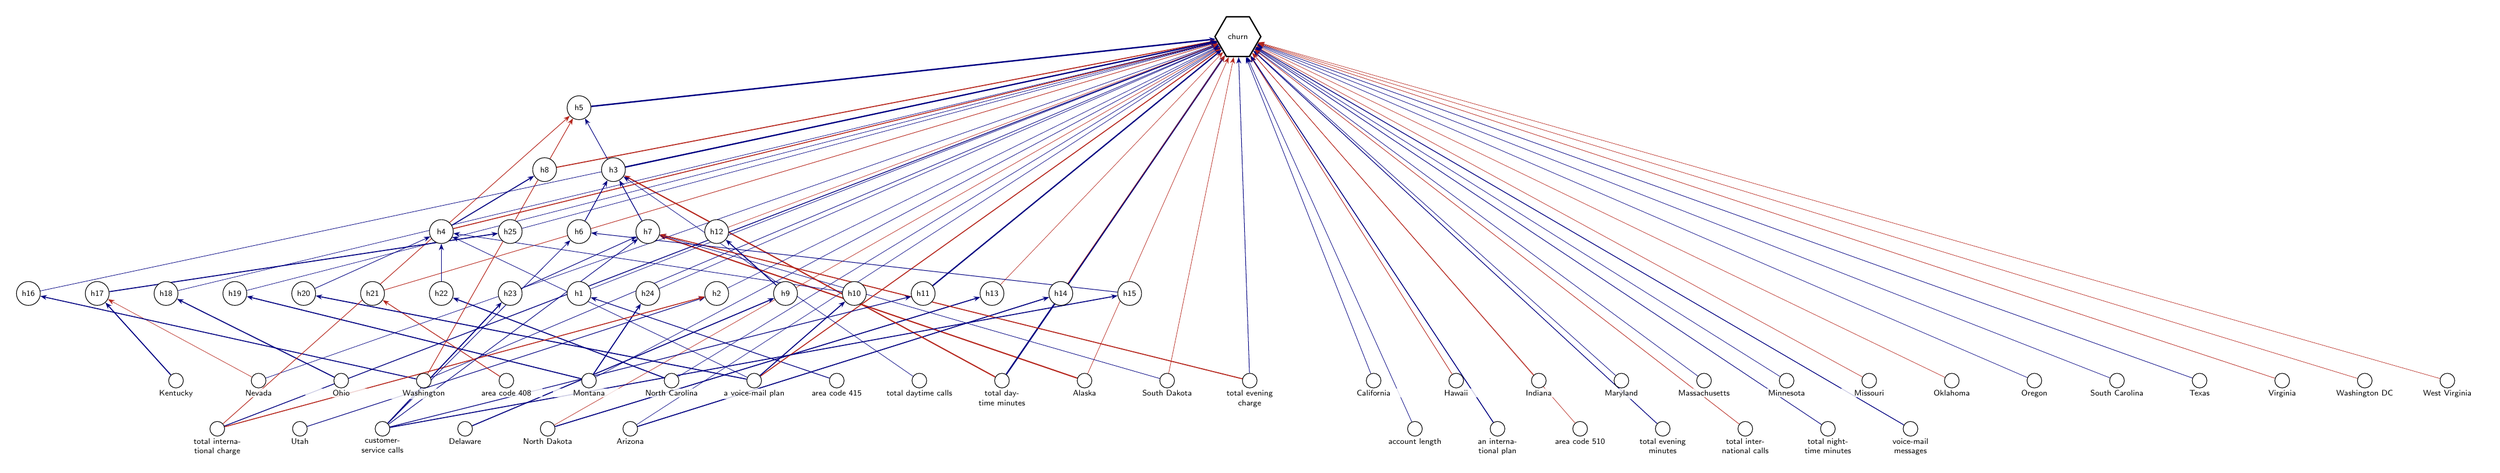
\begin{tikzpicture}[
  font=\sffamily\scriptsize, >={Stealth[length=1.4mm]},
  inp/.style={draw, circle, fill=white, minimum size=3.2mm, inner sep=0pt},
  hid/.style={draw, circle, fill=white, minimum size=5.2mm, inner sep=0.5pt, font=\sffamily\tiny},
  exitbox/.style={draw, thick, rectangle, fill=white, align=center, text width=17mm, minimum height=5mm, inner sep=1.5pt, font=\sffamily\tiny},
  sumbox/.style={draw, thick, dashed, rectangle, fill=white, align=center, text width=17mm, minimum height=5mm, inner sep=1.5pt, font=\sffamily\tiny},
  outp/.style={draw, thick, regular polygon, regular polygon sides=6, fill=white, minimum size=10mm, inner sep=0pt, font=\sffamily\tiny, align=center},
  stub/.style={draw, dashed, rounded corners=2pt, fill=white, align=center, inner sep=2pt, font=\sffamily\tiny, text width=15mm},
  inlab/.style={font=\sffamily\tiny, align=center, text width=15mm, inner sep=1pt, fill=white, fill opacity=0.8, text opacity=1},
  wpos/.style={draw=NavyBlue}, wneg/.style={draw=BrickRed}, wagg/.style={draw=black!45, line width=1.2pt},
  wmix/.style={draw=Plum},
]
\node[inp] (ninxxstatex17) at (0.0,0.0) {};
\path (ninxxstatex17.south) node[inlab, anchor=north] (labninxxstatex17) {Kentucky};
\node[inp] (ninxxstatex19) at (33.3,0.0) {};
\path (ninxxstatex19.south) node[inlab, anchor=north] (labninxxstatex19) {Massachusetts};
\node[inp] (ninxxstatex20) at (31.5,0.0) {};
\path (ninxxstatex20.south) node[inlab, anchor=north] (labninxxstatex20) {Maryland};
\node[inp] (ninxxstatex23) at (35.1,0.0) {};
\path (ninxxstatex23.south) node[inlab, anchor=north] (labninxxstatex23) {Minnesota};
\node[inp] (ninxxstatex24) at (36.9,0.0) {};
\path (ninxxstatex24.south) node[inlab, anchor=north] (labninxxstatex24) {Missouri};
\node[inp] (ninxxstatex0) at (19.8,0.0) {};
\path (ninxxstatex0.south) node[inlab, anchor=north] (labninxxstatex0) {Alaska};
\node[inp] (ninxxstatex26) at (9.0,0.0) {};
\path (ninxxstatex26.south) node[inlab, anchor=north] (labninxxstatex26) {Montana};
\node[inp] (ninxxstatex27) at (10.8,0.0) {};
\path (ninxxstatex27.south) node[inlab, anchor=north] (labninxxstatex27) {North Carolina};
\node[inp] (ninxxstatex28) at (8.1,-1.05) {};
\path (ninxxstatex28.south) node[inlab, anchor=north] (labninxxstatex28) {North Dakota};
\node[inp] (ninxxstatex3) at (9.9,-1.05) {};
\path (ninxxstatex3.south) node[inlab, anchor=north] (labninxxstatex3) {Arizona};
\node[inp] (ninxxstatex33) at (1.8,0.0) {};
\path (ninxxstatex33.south) node[inlab, anchor=north] (labninxxstatex33) {Nevada};
\node[inp] (ninxxstatex35) at (3.6,0.0) {};
\path (ninxxstatex35.south) node[inlab, anchor=north] (labninxxstatex35) {Ohio};
\node[inp] (ninxxstatex36) at (38.7,0.0) {};
\path (ninxxstatex36.south) node[inlab, anchor=north] (labninxxstatex36) {Oklahoma};
\node[inp] (ninxxstatex37) at (40.5,0.0) {};
\path (ninxxstatex37.south) node[inlab, anchor=north] (labninxxstatex37) {Oregon};
\node[inp] (ninxxstatex4) at (26.1,0.0) {};
\path (ninxxstatex4.south) node[inlab, anchor=north] (labninxxstatex4) {California};
\node[inp] (ninxxstatex40) at (42.3,0.0) {};
\path (ninxxstatex40.south) node[inlab, anchor=north] (labninxxstatex40) {South Carolina};
\node[inp] (ninxxstatex41) at (21.6,0.0) {};
\path (ninxxstatex41.south) node[inlab, anchor=north] (labninxxstatex41) {South Dakota};
\node[inp] (ninxxstatex43) at (44.1,0.0) {};
\path (ninxxstatex43.south) node[inlab, anchor=north] (labninxxstatex43) {Texas};
\node[inp] (ninxxstatex11) at (27.9,0.0) {};
\path (ninxxstatex11.south) node[inlab, anchor=north] (labninxxstatex11) {Hawaii};
\node[inp] (ninxxstatex44) at (2.7,-1.05) {};
\path (ninxxstatex44.south) node[inlab, anchor=north] (labninxxstatex44) {Utah};
\node[inp] (ninxxstatex45) at (45.9,0.0) {};
\path (ninxxstatex45.south) node[inlab, anchor=north] (labninxxstatex45) {Virginia};
\node[inp] (ninxxstatex47) at (5.4,0.0) {};
\path (ninxxstatex47.south) node[inlab, anchor=north] (labninxxstatex47) {Washington};
\node[inp] (ninxxstatex49) at (49.5,0.0) {};
\path (ninxxstatex49.south) node[inlab, anchor=north] (labninxxstatex49) {West Virginia};
\node[inp] (ninxxstatex7) at (47.7,0.0) {};
\path (ninxxstatex7.south) node[inlab, anchor=north] (labninxxstatex7) {Washington DC};
\node[inp] (ninxxstatex8) at (6.3,-1.05) {};
\path (ninxxstatex8.south) node[inlab, anchor=north] (labninxxstatex8) {Delaware};
\node[inp] (ninxxaccountxlength) at (27.0,-1.05) {};
\path (ninxxaccountxlength.south) node[inlab, anchor=north] (labninxxaccountxlength) {account length};
\node[inp] (ninxxareaxcodex408) at (7.2,0.0) {};
\path (ninxxareaxcodex408.south) node[inlab, anchor=north] (labninxxareaxcodex408) {area code 408};
\node[inp] (ninxxareaxcodex415) at (14.4,0.0) {};
\path (ninxxareaxcodex415.south) node[inlab, anchor=north] (labninxxareaxcodex415) {area code 415};
\node[inp] (ninxxareaxcodex510) at (30.6,-1.05) {};
\path (ninxxareaxcodex510.south) node[inlab, anchor=north] (labninxxareaxcodex510) {area code 510};
\node[inp] (ninxxinternationalxplan) at (28.8,-1.05) {};
\path (ninxxinternationalxplan.south) node[inlab, anchor=north] (labninxxinternationalxplan) {an international plan};
\node[inp] (ninxxvoicexmailxplan) at (12.6,0.0) {};
\path (ninxxvoicexmailxplan.south) node[inlab, anchor=north] (labninxxvoicexmailxplan) {a voice-mail plan};
\node[inp] (ninxxnumberxvmailxmessages) at (37.8,-1.05) {};
\path (ninxxnumberxvmailxmessages.south) node[inlab, anchor=north] (labninxxnumberxvmailxmessages) {voice-mail messages};
\node[inp] (ninxxtotalxdayxminutes) at (18.0,0.0) {};
\path (ninxxtotalxdayxminutes.south) node[inlab, anchor=north] (labninxxtotalxdayxminutes) {total daytime minutes};
\node[inp] (ninxxtotalxdayxcalls) at (16.2,0.0) {};
\path (ninxxtotalxdayxcalls.south) node[inlab, anchor=north] (labninxxtotalxdayxcalls) {total daytime calls};
\node[inp] (ninxxtotalxevexminutes) at (32.4,-1.05) {};
\path (ninxxtotalxevexminutes.south) node[inlab, anchor=north] (labninxxtotalxevexminutes) {total evening minutes};
\node[inp] (ninxxtotalxevexcharge) at (23.4,0.0) {};
\path (ninxxtotalxevexcharge.south) node[inlab, anchor=north] (labninxxtotalxevexcharge) {total evening charge};
\node[inp] (ninxxtotalxnightxminutes) at (36.0,-1.05) {};
\path (ninxxtotalxnightxminutes.south) node[inlab, anchor=north] (labninxxtotalxnightxminutes) {total night-time minutes};
\node[inp] (ninxxtotalxintlxcalls) at (34.2,-1.05) {};
\path (ninxxtotalxintlxcalls.south) node[inlab, anchor=north] (labninxxtotalxintlxcalls) {total international calls};
\node[inp] (ninxxtotalxintlxcharge) at (0.9,-1.05) {};
\path (ninxxtotalxintlxcharge.south) node[inlab, anchor=north] (labninxxtotalxintlxcharge) {total international charge};
\node[inp] (ninxxnumberxcustomerxservicexcalls) at (4.5,-1.05) {};
\path (ninxxnumberxcustomerxservicexcalls.south) node[inlab, anchor=north] (labninxxnumberxcustomerxservicexcalls) {customer-service calls};
\node[inp] (ninxxstatex15) at (29.7,0.0) {};
\path (ninxxstatex15.south) node[inlab, anchor=north] (labninxxstatex15) {Indiana};
\node[outp] (n0) at (23.142,7.5) {churn};
\node[hid] (n10332) at (-3.217,1.9) {h16};
\node[hid] (n11261) at (-1.717,1.9) {h17};
\node[hid] (n1133) at (5.783,3.25) {h4};
\node[hid] (n1264) at (8.783,5.95) {h5};
\node[hid] (n13551) at (-0.217,1.9) {h18};
\node[hid] (n13725) at (1.283,1.9) {h19};
\node[hid] (n13852) at (2.783,1.9) {h20};
\node[hid] (n14653) at (4.283,1.9) {h21};
\node[hid] (n14955) at (5.783,1.9) {h22};
\node[hid] (n15509) at (7.283,1.9) {h23};
\node[hid] (n161) at (8.783,1.9) {h1};
\node[hid] (n16344) at (10.283,1.9) {h24};
\node[hid] (n16902) at (7.283,3.25) {h25};
\node[hid] (n252) at (11.783,1.9) {h2};
\node[hid] (n2627) at (8.783,3.25) {h6};
\node[hid] (n2796) at (10.283,3.25) {h7};
\node[hid] (n4051) at (8.033,4.6) {h8};
\node[hid] (n4967) at (13.283,1.9) {h9};
\node[hid] (n5577) at (14.783,1.9) {h10};
\node[hid] (n7208) at (16.283,1.9) {h11};
\node[hid] (n7647) at (11.783,3.25) {h12};
\node[hid] (n807) at (9.533,4.6) {h3};
\node[hid] (n8418) at (17.783,1.9) {h13};
\node[hid] (n8896) at (19.283,1.9) {h14};
\node[hid] (n9555) at (20.783,1.9) {h15};
\begin{scope}[on background layer]
\draw[->, wneg, line width=0.27pt] (ninxxstatex0) -- (n0);
\draw[->, wneg, line width=0.74pt] (ninxxstatex0) -- (n2796);
\draw[->, wpos, line width=0.60pt] (ninxxstatex17) -- (n11261);
\draw[->, wpos, line width=0.27pt] (ninxxstatex19) -- (n0);
\draw[->, wpos, line width=0.28pt] (ninxxstatex20) -- (n0);
\draw[->, wpos, line width=0.27pt] (ninxxstatex23) -- (n0);
\draw[->, wneg, line width=0.26pt] (ninxxstatex24) -- (n0);
\draw[->, wpos, line width=0.27pt] (ninxxstatex26) -- (n0);
\draw[->, wpos, line width=0.60pt] (ninxxstatex26) -- (n13725);
\draw[->, wpos, line width=0.60pt] (ninxxstatex26) -- (n16344);
\draw[->, wpos, line width=0.26pt] (ninxxstatex27) -- (n0);
\draw[->, wpos, line width=0.60pt] (ninxxstatex27) -- (n14955);
\draw[->, wneg, line width=0.26pt] (ninxxstatex28) -- (n0);
\draw[->, wpos, line width=0.60pt] (ninxxstatex28) -- (n8418);
\draw[->, wpos, line width=0.25pt] (ninxxstatex3) -- (n0);
\draw[->, wpos, line width=0.60pt] (ninxxstatex3) -- (n8896);
\draw[->, wpos, line width=0.27pt] (ninxxstatex33) -- (n0);
\draw[->, wneg, line width=0.26pt] (ninxxstatex33) -- (n11261);
\draw[->, wpos, line width=0.60pt] (ninxxstatex35) -- (n13551);
\draw[->, wneg, line width=0.25pt] (ninxxstatex36) -- (n0);
\draw[->, wpos, line width=0.26pt] (ninxxstatex37) -- (n0);
\draw[->, wpos, line width=0.30pt] (ninxxstatex4) -- (n0);
\draw[->, wpos, line width=0.27pt] (ninxxstatex40) -- (n0);
\draw[->, wneg, line width=0.28pt] (ninxxstatex41) -- (n0);
\draw[->, wpos, line width=0.30pt] (ninxxstatex41) -- (n2796);
\draw[->, wpos, line width=0.30pt] (ninxxstatex43) -- (n0);
\draw[->, wneg, line width=0.34pt] (ninxxstatex11) -- (n0);
\draw[->, wpos, line width=0.40pt] (ninxxstatex44) -- (n252);
\draw[->, wneg, line width=0.29pt] (ninxxstatex45) -- (n0);
\draw[->, wpos, line width=0.31pt] (ninxxstatex47) -- (n0);
\draw[->, wpos, line width=0.56pt] (ninxxstatex47) -- (n10332);
\draw[->, wneg, line width=0.39pt] (ninxxstatex47) -- (n1264);
\draw[->, wneg, line width=0.25pt] (ninxxstatex49) -- (n0);
\draw[->, wneg, line width=0.26pt] (ninxxstatex7) -- (n0);
\draw[->, wpos, line width=0.59pt] (ninxxstatex8) -- (n4967);
\draw[->, wpos, line width=0.29pt] (ninxxaccountxlength) -- (n0);
\draw[->, wneg, line width=0.44pt] (ninxxareaxcodex408) -- (n14653);
\draw[->, wpos, line width=0.45pt] (ninxxareaxcodex415) -- (n161);
\draw[->, wneg, line width=0.26pt] (ninxxareaxcodex510) -- (n0);
\draw[->, wpos, line width=0.52pt] (ninxxinternationalxplan) -- (n0);
\draw[->, wneg, line width=0.56pt] (ninxxvoicexmailxplan) -- (n0);
\draw[->, wpos, line width=0.29pt] (ninxxvoicexmailxplan) -- (n1133);
\draw[->, wpos, line width=0.60pt] (ninxxvoicexmailxplan) -- (n13852);
\draw[->, wpos, line width=0.59pt] (ninxxvoicexmailxplan) -- (n5577);
\draw[->, wpos, line width=0.45pt] (ninxxnumberxvmailxmessages) -- (n0);
\draw[->, wpos, line width=0.90pt] (ninxxtotalxdayxminutes) -- (n0);
\draw[->, wneg, line width=0.71pt] (ninxxtotalxdayxminutes) -- (n807);
\draw[->, wpos, line width=0.27pt] (ninxxtotalxdayxcalls) -- (n807);
\draw[->, wpos, line width=0.42pt] (ninxxtotalxevexminutes) -- (n0);
\draw[->, wpos, line width=0.37pt] (ninxxtotalxevexcharge) -- (n0);
\draw[->, wneg, line width=0.60pt] (ninxxtotalxevexcharge) -- (n2796);
\draw[->, wpos, line width=0.35pt] (ninxxtotalxnightxminutes) -- (n0);
\draw[->, wneg, line width=0.31pt] (ninxxtotalxintlxcalls) -- (n0);
\draw[->, wpos, line width=0.49pt] (ninxxtotalxintlxcharge) -- (n0);
\draw[->, wneg, line width=0.37pt] (ninxxtotalxintlxcharge) -- (n1264);
\draw[->, wneg, line width=0.55pt] (ninxxtotalxintlxcharge) -- (n252);
\draw[->, wpos, line width=0.60pt] (ninxxnumberxcustomerxservicexcalls) -- (n15509);
\draw[->, wpos, line width=0.33pt] (ninxxnumberxcustomerxservicexcalls) -- (n2627);
\draw[->, wpos, line width=0.36pt] (ninxxnumberxcustomerxservicexcalls) -- (n2796);
\draw[->, wpos, line width=0.45pt] (ninxxnumberxcustomerxservicexcalls) -- (n7208);
\draw[->, wpos, line width=0.57pt] (ninxxnumberxcustomerxservicexcalls) -- (n9555);
\draw[->, wneg, line width=0.25pt] (ninxxstatex15) -- (n0);
\draw[->, wpos, line width=0.29pt] (n10332) -- (n0);
\draw[->, wpos, line width=0.60pt] (n11261) -- (n16902);
\draw[->, wneg, line width=0.56pt] (n1133) -- (n0);
\draw[->, wpos, line width=0.58pt] (n1133) -- (n4051);
\draw[->, wpos, line width=0.88pt] (n1264) -- (n0);
\draw[->, wpos, line width=0.27pt] (n13551) -- (n0);
\draw[->, wpos, line width=0.27pt] (n13725) -- (n0);
\draw[->, wpos, line width=0.33pt] (n13852) -- (n1133);
\draw[->, wneg, line width=0.34pt] (n14653) -- (n0);
\draw[->, wpos, line width=0.26pt] (n14955) -- (n1133);
\draw[->, wpos, line width=0.38pt] (n15509) -- (n2796);
\draw[->, wpos, line width=0.27pt] (n161) -- (n0);
\draw[->, wpos, line width=0.27pt] (n16344) -- (n0);
\draw[->, wpos, line width=0.27pt] (n16902) -- (n0);
\draw[->, wpos, line width=0.25pt] (n252) -- (n0);
\draw[->, wpos, line width=0.46pt] (n2627) -- (n807);
\draw[->, wpos, line width=0.45pt] (n2796) -- (n807);
\draw[->, wneg, line width=0.60pt] (n4051) -- (n0);
\draw[->, wpos, line width=0.59pt] (n4967) -- (n7647);
\draw[->, wpos, line width=0.32pt] (n5577) -- (n1133);
\draw[->, wpos, line width=0.78pt] (n7208) -- (n0);
\draw[->, wneg, line width=0.25pt] (n7647) -- (n0);
\draw[->, wpos, line width=0.80pt] (n807) -- (n0);
\draw[->, wpos, line width=0.37pt] (n807) -- (n1264);
\draw[->, wneg, line width=0.25pt] (n8418) -- (n0);
\draw[->, wneg, line width=0.25pt] (n8896) -- (n0);
\draw[->, wpos, line width=0.38pt] (n9555) -- (n2627);
\end{scope}
\end{tikzpicture}}%
\caption{The network as trained, before any explanation, in full. Blue: positive weight (raises the score); red: negative weight (lowers it); thicker: larger weight. Orange outline and up arrow: raises the final prediction; teal and down arrow: lowers it; grey and double arrow: depends. Not used (no connection): Alabama, Georgia, Iowa, Idaho, Illinois, Kansas, Louisiana, Arkansas, Maine, Michigan, Mississippi, Nebraska, New Hampshire, New Jersey, New Mexico, New York, Pennsylvania, Rhode Island, Tennessee, Vermont, Wisconsin, Colorado, Wyoming, Connecticut, Florida, total daytime charge, total evening calls, total night-time calls, total night-time charge, total international minutes.}
\label{fig:churn100s2c2:raw}
\end{figure}
\end{landscape}
\end{drafted}
\clearpage
\end{document}
